\documentclass[11pt]{article}
\pdfinfoomitdate=1
\pdftrailerid{}
\pdfsuppressptexinfo=15
\usepackage[T1]{fontenc}
\usepackage[utf8]{inputenc}
\usepackage{lmodern}
\usepackage[a4paper,margin=29mm]{geometry}
\usepackage{amsmath,amssymb,amsthm,mathtools}
\usepackage{microtype}
\usepackage{enumitem,booktabs,array}
\usepackage{xcolor}
\usepackage{tikz}
\usetikzlibrary{arrows.meta,positioning}
\usepackage{xurl}
\usepackage[nottoc,notlof,notlot]{tocbibind}
\usepackage{hyperref}
\hypersetup{colorlinks=true,linkcolor=blue!45!black,citecolor=blue!45!black,urlcolor=blue!45!black,
  pdftitle={Hilbert's tenth problem over the rational numbers},pdfauthor={OpenAI},pdflang={en}}
\urlstyle{same}
\newcommand{\bibdoi}[1]{\href{https://doi.org/#1}{doi:\nolinkurl{#1}}}
\setlength{\emergencystretch}{2em}
\numberwithin{equation}{section}
\newtheorem{theorem}{Theorem}[section]
\newtheorem{proposition}[theorem]{Proposition}
\newtheorem{lemma}[theorem]{Lemma}
\newtheorem{corollary}[theorem]{Corollary}
\theoremstyle{definition}
\newtheorem{definition}[theorem]{Definition}
\newtheorem{remark}[theorem]{Remark}
\newtheorem{notation}[theorem]{Notation}
\newcommand{\Q}{\mathbb Q}
\newcommand{\Z}{\mathbb Z}
\newcommand{\N}{\mathbb N}
\newcommand{\F}{\mathbb F}
\newcommand{\R}{\mathbb R}
\newcommand{\C}{\mathbb C}
\newcommand{\hgt}{h}
\newcommand{\Sha}{\mathop{\mathrm{Sha}}}
\DeclareMathOperator{\Sel}{Sel}
\DeclareMathOperator{\rank}{rank}
\DeclareMathOperator{\corank}{corank}
\DeclareMathOperator{\ord}{ord}
\DeclareMathOperator{\rad}{rad}
\DeclareMathOperator{\Gal}{Gal}
\DeclareMathOperator{\End}{End}
\DeclareMathOperator{\Hom}{Hom}
\DeclareMathOperator{\Frac}{Frac}
\DeclareMathOperator{\Supp}{Supp}
\DeclareMathOperator{\im}{im}
\DeclareMathOperator{\coker}{coker}
\DeclareMathOperator{\Br}{Br}
\DeclareMathOperator{\GL}{GL}
\DeclareMathOperator{\GSp}{GSp}
\DeclareMathOperator{\Trd}{Trd}
\DeclareMathOperator{\Nrd}{Nrd}
\newcommand{\st}{^{*}}
\title{Hilbert's tenth problem over the rational numbers}
\author{OpenAI}
\date{October 6, 2026}
\begin{document}
\maketitle
\begin{abstract}
We give a negative answer to Hilbert's tenth problem over the rational numbers:
no algorithm decides whether a polynomial with integer coefficients has a rational
zero. The number of variables is part of the input.
\end{abstract}
\clearpage
{\small\setlength{\parskip}{0pt}\tableofcontents}
\clearpage
\section{Introduction}\label{sec:introduction}

Hilbert's tenth problem over the rational numbers asks for a decision
procedure for rational zeros of polynomials with integer coefficients.
The number of variables is part of the input.

\begin{theorem}\label{thm:main}
There is no algorithm which, given a polynomial
$f\in\Z[X_1,\ldots,X_n]$, with $n$ part of the input, decides whether
$f$ has a zero in $\Q^n$.
\end{theorem}

\subsection{Historical setting}

Hilbert's tenth problem, as stated in his 1900 list of mathematical
problems, asks for a finite procedure deciding whether a polynomial
equation with integer coefficients has a solution in the ordinary
integers \cite[Problem~10]{Hilbert1900}.  Its negative resolution grew
out of a much stronger description of polynomial equations.  A relation
on the positive integers is \emph{recursively enumerable} if an
algorithm can list exactly its satisfying tuples.  It is
\emph{Diophantine} if membership can be expressed by the existence of
additional positive integers satisfying a polynomial equation with
integer coefficients.  Thus a Diophantine description expresses a
condition entirely through polynomial solvability.

Davis, Putnam, and Robinson proved in 1961 that every recursively
enumerable relation has such a representation if exponentiation is
also allowed.  They reduced the ordinary polynomial representation
theorem to a growth criterion for a Diophantine relation
\cite[Theorem and Corollary~3]{DavisPutnamRobinson1961}.
Matiyasevich supplied the required growth in 1970 through a
Diophantine description of a Fibonacci relation, completing the
theorem that every recursively enumerable relation on the positive
integers is Diophantine \cite{Matiyasevich1970}.  The equivalent
all-integer decision problem is therefore undecidable.  This
representation theorem explains the strength of the result: integer
polynomial equations can encode arbitrary recursively enumerable
conditions.

Letting the unknowns range over \(\mathbb Q\) changes the decision
problem.  Enumerating rational tuples will eventually find any rational
zero, but gives no answer for an equation without one.  A possible
transfer of the integer theorem would be an existential definition of
membership in \(\mathbb Z\) using only the ring operations of
\(\mathbb Q\).  One could then replace each integer unknown by a
rational unknown subject to that membership condition, obtaining an
equivalent rational existential question.  More generally, a
\emph{Diophantine model} of integer arithmetic represents the integers
by a Diophantine subset of some \(\mathbb Q^k\), with Diophantine
relations for addition and multiplication.  Such a model also
translates integer equations into rational existential questions
\cite[Definition~3.1 and Observation~3.3]{CornelissenZahidi2000}.
Here the defining polynomial equations and all their witnesses are
interpreted over \(\mathbb Q\).
These constructions are sufficient routes to undecidability; the
decision problem does not require its solution to produce either one.

Julia Robinson showed in 1949 that the integers are first-order
definable in the rationals using addition and multiplication.  Her
formula uses both universal and existential quantifiers, and her work
also proves undecidability of the full first-order theory of rational
arithmetic \cite[Theorems~3.1 and~4.2]{Robinson1949}.  Later work
reduced the quantifier complexity.  Poonen defined \(\mathbb Z\) in
\(\mathbb Q\) by a positive formula with two universal quantifiers
followed by seven existential quantifiers
\cite[Theorem~4.1]{Poonen2009}.  Koenigsmann then gave a universal
definition of \(\mathbb Z\); equivalently, its complement in
\(\mathbb Q\) is Diophantine.  His result also implies undecidability
of the \(\forall\exists\) theory
\cite[Theorem~1 and Corollaries~2--3]{Koenigsmann2016}.  These results
give substantial control of definitions inside \(\mathbb Q\), but
do not supply the existential membership condition for the direct
transfer above.

The distinction between a Diophantine model and undecidability also
has a geometric setting.  Mazur conjectured that, for a variety over
\(\mathbb Q\), the closure of its rational points in its real points
has only finitely many connected components
\cite[Conjecture~3]{Mazur1995}.  He observed that this conjecture
would rule out a Diophantine definition of \(\mathbb Z\) in
\(\mathbb Q\).  Cornelissen and Zahidi showed that it would also rule
out a Diophantine model of integer arithmetic in a finite Cartesian
power of \(\mathbb Q\)
\cite[Theorem~3.6]{CornelissenZahidi2000}.  These obstructions to
definitions and models do not by themselves rule out a negative
answer to the rational decision problem.

One approach studies the subrings
\(\mathbb Z[S^{-1}]\subseteq\mathbb Q\), whose denominators use only
primes in \(S\).  Poonen constructed disjoint recursive sets of primes
\(T_1,T_2\), each of natural density zero, such that positive-integer
arithmetic has a Diophantine model in \(\mathbb Z[S^{-1}]\) whenever
\(S\supseteq T_1\) and \(S\cap T_2=\varnothing\).  Hilbert's tenth
problem is undecidable for every such ring.  Taking \(S\) to be the
complement of \(T_2\) gives a recursive set of density one and a
proper subring of \(\mathbb Q\)
\cite[Theorem~1.3]{PoonenSubrings}.  The construction uses selected
multiples of a point on a rank-one elliptic curve whose real
coordinates approximate integers.  

Eisenträger, Miller, Park, and Shlapentokh later constructed
computably presentable subrings \(\mathbb Z[S^{-1}]\), including
examples in which \(S\) has density one, whose Hilbert's tenth problem
is Turing equivalent to that over \(\mathbb Q\)
\cite[Theorem~3.17]{EisentragerMillerParkShlapentokh2017}.  For these
examples, a Turing reduction from integer solvability would already
give a Turing reduction from integer solvability to the rational
field problem.  The density of the
inverted primes alone therefore does not settle the relation to the
field problem.

Elliptic curves also give a transfer between rings of integers of
number fields.  Poonen proved that, for \(F\subseteq K\), an elliptic
curve \(E/F\) with
\[
             \operatorname{rank}E(F)=\operatorname{rank}E(K)=1
\]
makes \(\mathcal O_F\) Diophantine in \(\mathcal O_K\)
\cite[Theorem~1]{PoonenRankOne2002}.  If \(\mathbb Z\) is already
Diophantine in \(\mathcal O_F\), undecidability transfers to
\(\mathcal O_K\).  Mazur and Rubin pursued this route through
quadratic twists and Selmer groups, conditional on the conjectured
evenness of \(\dim_{\mathbb F_2}\operatorname{Sha}(E/L)[2]\).
Assuming this for every elliptic curve over every number field, they obtained undecidability for
every infinite finitely generated \(\mathbb Z\)-algebra
\cite[Theorem~1.13, Corollary~1.14, and Theorem~8.1]{MazurRubin2010}.

This number-field program has recently been completed
unconditionally.  Koymans and Pagano combined two-descent with
additive combinatorics to prove that \(\mathbb Z\) is Diophantine in
the ring of integers of every number field, and that Hilbert's tenth
problem is undecidable for every infinite finitely generated
\(\mathbb Z\)-algebra \cite{KoymansPagano2026}.
Alpöge, Bhargava, Ho, and Shnidman
gave another route: for every quadratic extension \(K/F\) of number fields, they
construct an abelian variety over \(F\) with positive rank unchanged
over \(K\), and deduce that \(\mathbb Z\) is Diophantine in every
number-field ring of integers
\cite[Theorem~1.1 and Corollary~1.2]{AlpogeBhargavaHoShnidman2026}.
The field \(\mathbb Q\) is not a finitely generated
\(\mathbb Z\)-algebra, so these results concern a different class of
rings from the field in Theorem~\ref{thm:main}.

The elliptic approach also illuminates nearby rational decision
problems.  In a rank-one group, a multiple \(nP\) of a nontorsion
point can represent the integer \(n\), and local coordinates or heights can reveal arithmetic
information about that index.  Cornelissen and Zahidi used elliptic
divisibility sequences and existential valuation predicates in this
direction.  Under a conjectural odd primitive-divisor property for one
such sequence, they obtained a Diophantine model of
\((\mathbb Z,+,\mid)\) and proved undecidability of a positive
\(\Pi_2\) fragment with one universal quantifier
\cite[Conjecture~3.16 and Theorems~3.17 and~5.3]{CornelissenZahidi2007}.
The assertion with one universal quantifier uses the correction by
Cornelissen and Shlapentokh
\cite[Remark~2.3 in the author version]{CornelissenShlapentokh2009}.


Garcia-Fritz, Pasten, and Vidaux instead adjoined predicates comparing
the logarithmic heights of rational tuples to the rational ring
language.  In this expanded language they gave a
positive existential interpretation of \(\mathbb N\), and hence
proved undecidability; comparisons between tuples of length at most
three suffice \cite[Theorems~1.1--1.2]{GarciaFritzPastenVidaux2025}.
Their construction uses elliptic canonical heights to encode
consecutive squares.  The present paper concerns ordinary rational
polynomial solvability, and its height estimates enter the proof of
that ordinary statement.

\subsection{Proof strategy}

Constant polynomials can be decided directly. For each nonconstant integral
polynomial \(f\), we construct an effectively generated sequence of finite tests.
Each test can be answered by finitely many rational-solvability queries, and the sequence satisfies
\begin{equation}\label{intro:finite-test-interface}
 f\text{ has an integer zero}
 \quad\Longleftrightarrow\quad
 \text{every test succeeds}.
\end{equation}
An integer zero supplies witnesses for all the tests. If a rational-solvability algorithm existed, we could run two searches in parallel: enumeration of integer zeros, and enumeration of tests until one fails. The arithmetic work is to prove that a failed test exists whenever \(f\) has no integer zero.

Suppose all the finite tests succeed. Compactness then gives a ring \(R\) containing a zero \(\mathbf a=(a_1,\ldots,a_n)\) of \(f\), embedded in an elementary extension of the rational field; we use a tilde for embedded values and points. The ambient extension also carries the integer and valuation data, height functions, elliptic multiple maps, and functions for finite products used in the proof. The tests attach an elliptic point \(T_a\) to each \(a\in R\), compatibly with addition, and require \(T_a\) to be nonidentity when \(a\ne0\). The embedded points lie in the transferred copy of a fixed infinite cyclic subgroup \(\Z P\) of finite index in a rank-one elliptic group, with \(T_1=P\). This defines unique indices
\[
                 \widetilde T_a=\eta(a)P,
                 \qquad \eta(a)\in{}^*\Z.
\]
Here \({}^*\Z\) is the ambient integer structure, whose elements may be nonordinary. The point axioms make \(\eta:R\to{}^*\Z\) injective and additive, with \(\eta(1)=1\), but \(\eta\) need not respect multiplication. Thus the modeled equation does not yet give an equation satisfied by the indices.

Two local comparisons address this obstruction. The primary test compares an embedded ring value with a quotient of truncated elliptic logarithms. The formal logarithm can recover the corresponding quotient of point indices once that quotient is integral at the prime. A second comparison, on the conjugate elliptic curve, supplies this control using only additivity of \(\eta\). Where the comparisons apply, they show that every \(\widetilde a\) is integral at the prime and agrees with \(\eta(a)\) to the prescribed precision. Each pair uses auxiliary choices that work for every ring element, which is essential for the later uniform bound.

The proof arranges these comparisons at primes detected by a height estimate. Fix the five rational points of \(\mathbf P^1\) supplied by that estimate and primitive integral linear forms vanishing at them; call these the contact forms. For a rational point \(s=(u:v)\) outside this set, written in coprime integer coordinates, let \(M(s)\) be the product, without repetition, of the nonexceptional primes at which one of these forms has odd valuation. We call the primes counted by \(M(s)\) its contact primes. The estimate bounds the absolute logarithmic Weil height by
\[
                              h(s)\le H M(s)^c
\]
for fixed constants \(H,c\). This definition and estimate transfer to the ambient extension. At each prescribed precision, the theory represents every ring element as a
sum of three fractions of ring elements, called slopes, and equips factors of
their contact forms with the local conditions. A prime-pattern theorem supplies
the required primes for these representations in the ordinary integer model.
A separate existential condition controls the parity of possible denominator
valuations outside a fixed finite set. In a model satisfying the tests, consider
the three slopes supplied for any ring element at that precision. After the
further fixed exclusions, the parity condition lets the proof apply the local
comparisons at every contact prime of those slopes. Enlarging the exceptional
set changes the height constant but preserves the exponent \(c\).

Set
\[
 \delta=f\bigl(\eta(a_1),\ldots,\eta(a_n)\bigr),
 \qquad
 B=\max\bigl(1,|\eta(a_1)|,\ldots,|\eta(a_n)|\bigr).
\]
If \(\delta=0\), elementarity gives an ordinary integer zero of \(f\). Otherwise \(\delta\) is a nonzero ambient integer whose size is bounded by a fixed polynomial in \(B\). Choose one ordinary precision \(K\) large enough in terms of the degree of \(f\) and the exponent \(c\). For any \(A\in R\), choose a tested representation at precision \(K\). Every contact prime of its slopes divides this same \(\delta\) to order at least \(K\), because all modeled root coordinates agree locally with their indices. The height estimate then bounds each slope height by a constant times \(B\). The logarithmic height inequality for their sum gives
\[
                         h(\widetilde A)\ll_f B
                         \qquad\text{for every }A\in R,
\]
with one ordinary constant.

For each nonzero root coordinate \(a_j\), consider its attached point
\(T_{a_j}\). Applying the uniform bound to the ring elements representing
\(x(T_{a_j})\) gives \(h(x(\eta(a_j)P))\ll_f B\).
The transferred canonical-height comparison for \(P\) makes this height grow
quadratically in \(|\eta(a_j)|\). If \(B>1\), choose \(j\) with
\(|\eta(a_j)|=B\); the two bounds give \(B^2\ll_f B\). If \(B=1\), the
required bound is immediate. Thus all root indices lie in an ordinary finite
interval. Additivity and injectivity identify the modeled root coordinates
with those ordinary integers, contradicting \(\delta\ne0\). This proves the
finite-test equivalence and hence the undecidability theorem.

The detailed reduction in Section~\ref{sec:reduction} makes these steps
precise. Section~\ref{par:section} proves the pole-parity condition; its
passage from two-descent data to rational points uses the pointwise
$2$-converse \cite[Theorem~1.1]{PointwiseTwoConverse} and the
Cassels--Tate pairing \cite{Cassels1962}.
Section~\ref{hei:section} proves the five-point height estimate. Its
modularity step uses the odd regular Fontaine--Mazur theorem at $2$
\cite[Theorem~1.1]{OddRegularFontaineMazurAtTwo}, whose statement has no
hypothesis on the residual image. Section~\ref{ell:section} proves the
rank-one and local elliptic results, and Section~\ref{pri:section}
supplies the prime patterns and simultaneous local witnesses for the
ordinary integer model. Section~\ref{red:degree-normal-form} gives
Turing degree $0'$ and the quartic normal form.

At rational primes, valuations are normalized by \(v_q(q)=1\), with
\(v_q(0)=+\infty\). The support of a nonzero rational number is the set of
primes dividing its numerator or denominator in lowest terms. The notation
\(X\ll Y\) means \(X\le CY\) for a positive constant depending only on the
fixed data in the statement; additional dependencies are indicated when
they occur.

\section{Finite rational tests for integer solvability}
\label{sec:reduction}

We construct the finite rational tests announced in the introduction and
prove that success of every test forces an ordinary integer zero.  The
construction has an ordinary integer model.  Conversely, compactness will
embed a model of all the tests in an elementary extension of \(\Q\),
where arithmetic restrictions on its ring values will force an integer
solution.  The later sections prove the arithmetic inputs used here.

The elliptic point data first give an additive assignment of integer
indices.  A local comparison will recover those indices from ring values
and determine the two local test conditions.

\subsection{Elliptic indices and the local comparison}
\label{red:local-comparison-section}

Fix the number field, involution, and elliptic curve
\begin{equation}\label{ell:data}
 F=\Q(\sqrt2),\qquad d=75-53\sqrt2,\qquad
 E:\ y^2=x^3-d^2x,
\end{equation}
where \(\sigma\) is the nontrivial automorphism of \(F/\Q\).
The following result, proved in Section~\ref{ell:section}, supplies the
integer indices.

\begin{proposition}\label{ell:rank}
The group $E(F)$ has rank one.  Consequently there exist a positive integer
$m$ and a nontorsion point $P\in E(F)$ such that
\[
                         mE(F)=\Z P.
\]
We fix such $m$ and $P$ once and for all.
\end{proposition}

We now describe the point data that the recursive theory will impose.
Let \(R\) be an integral domain
of characteristic zero for which \(\sqrt2\notin\Frac(R)\), and write
\[
 R_F=R[\sqrt2],\qquad F_R=\Frac(R)(\sqrt2).
\]
For each \(a\in R\), consider a point \(T_a\in E(F_R)\) subject to
\begin{equation}\label{red:elliptic-axioms}
\begin{gathered}
 T_0=O,\qquad T_1=P,\qquad
 T_{a+a'}=T_a+T_{a'}\quad(a,a'\in R),\\
 T_a\in mE(F_R)\quad(a\in R),\\
 a\ne0\Longrightarrow T_a\text{ is finite and }x(T_a)y(T_a)\ne0.
\end{gathered}
\end{equation}
The theory will supply six unary ring-valued functions
\(x_0,x_1,x_2,y_0,y_1,y_2\). For \(a\ne0\), they are required to
satisfy \(x_2(a)y_2(a)\ne0\) and
\begin{equation}\label{red:coordinate-functions}
 x(T_a)=\frac{x_0(a)+x_1(a)\sqrt2}{x_2(a)},\qquad
 y(T_a)=\frac{y_0(a)+y_1(a)\sqrt2}{y_2(a)}.
\end{equation}
Their values at \(a=0\) are unrestricted, since \(T_0=O\).
In the integer model we will take \(T_a=aP\). Representing the
coordinates by ring elements will also let a uniform height bound on
\(R\) control their heights.

For the arithmetic analysis, consider an elementary extension of the
ordinary many-sorted structure containing \(\Q,\Z,\R,F\), the prime and
valuation relations, the height functions, the elliptic multiple maps,
and the finite-product functions. We call elements of the original
structure \emph{ordinary}; starred sorts satisfy the same first-order
statements with ordinary parameters. For the moment, suppose that \(R\)
embeds in the rational sort \({}^*\Q\) of such an extension. Its
fraction-field interpretation embeds \(F_R\) in \({}^*F\). A tilde
denotes the image of a ring element, field element, or point. Later
compactness will supply an extension and an embedded ring with these
properties.

The identity \(mE(F)=\Z P\) transfers to this extension: every point
of \(mE({}^*F)\) has a unique expression \(nP\), with
\(n\in{}^*\Z\). Define
\begin{equation}\label{red:eta}
                         \widetilde T_a=\eta(a)P.
\end{equation}
The group-law axioms give
\begin{equation}\label{red:additivity}
       \eta(a+a')=\eta(a)+\eta(a'),\qquad \eta(1)=1.
\end{equation}
If \(\eta(a)=0\), then \(T_a=O\), and the finite-point axiom forces
\(a=0\). Thus \(\eta:R\to{}^*\Z\) is injective and additive.
Conjugating \eqref{red:eta} gives
\(\widetilde T_a^\sigma=\eta(a)P^\sigma\).
We make no assumption about \(\eta(aa')\).

For nonzero \(h\in R\), the index ratio of \(T_{ha}\) and \(T_h\) is
\(\eta(ha)/\eta(h)\), which need not equal \(\eta(a)\).  We will
recover this ratio locally from point parameters, and use a second
comparison to identify it with \(\eta(a)\) to the required precision.

For a finite point with \(y\ne0\), put \(z=-x/y\), and set \(z(O)=0\).
Every nonzero multiple of \(P\) avoids the two-torsion points, so
\(z(nP)\) is defined for every integer \(n\).  Write
\[
 \ell(Z)=Z+\sum_{t\ge2}c_tZ^t\in F[[Z]],\qquad
 \ell_K(Z)=Z+\sum_{2\le t\le K}c_tZ^t
\]
for the formal logarithm in this parameter and its truncation through
degree \(K\).  The truncations are effectively computable from the
fixed equation.  Section~\ref{ell:section} proves the following uniform
statements about integer multiples of the fixed \(F\)-rational points
\(P,P^\sigma\).

\begin{proposition}\label{ell:formal}
There is a fixed finite set of rational primes $S_E$ with the following
properties.  Let $p\notin S_E$, let $v$ be any place of $F$ above $p$,
normalized by $v(p)=1$, and let $n,n'\in\Z$, with $n'\ne0$.  Assume
$nP,n'P$ reduce to $O$ at $v$.  Then
\begin{equation}\label{ell:ratio}
           v\!\left(\frac{z(nP)}{z(n'P)}\right)=v_p(n/n').
\end{equation}
For every integer $K\ge1$, if in addition $p>K+1$ and $v_p(n/n')\ge0$,
then $\ell_K(z(n'P))\ne0$ and
\begin{equation}\label{ell:truncation}
 v\!\left(\frac{\ell_K(z(nP))}{\ell_K(z(n'P))}-\frac n{n'}\right)
                         \ge K.
\end{equation}
Both assertions also hold at the same place $v$ after replacing
$E,P,\ell_K$ by $E^\sigma,P^\sigma,\ell_K^\sigma$ and imposing the
corresponding reduction-to-$O$ hypotheses on the conjugate points.
Here and below the valuation of zero is $+\infty$, so $n=0$ is included.
\end{proposition}

The two estimates provide different kinds of local information. Equation
\eqref{ell:ratio} determines the valuation of an index ratio from the
point parameters without assuming that the ratio is integral. Once an
index ratio is known to be integral, \eqref{ell:truncation} approximates
it by a ratio of finite polynomial evaluations. The next lemma combines both forms of control.

Reduction to \(O\) has its usual valuation meaning, transferred to the
elementary extension.
Only the stated assertions about integer multiples of the fixed
\(F\)-rational points \(P,P^\sigma\) and evaluations of the finite
polynomials \(\ell_K,\ell_K^\sigma\) are transferred; no infinite
formal series is evaluated in the extension.

\begin{samepage}
\begin{lemma}[Local comparison]\label{red:local-comparison}
Let \(K\ge1\) be an ordinary integer. Let \(q\) be a prime of the
ambient integer sort \({}^*\Z\), possibly nonordinary, with
\(q\notin S_E\) and \(q>K+1\), and let \(v_*\) be a place of
\({}^*F\) above \(q\), normalized by \(v_*(q)=1\).
Suppose there are nonzero \(h,j_0\in R\), chosen independently of
\(a\), such that for every \(a\in R\):
\begin{enumerate}[label=(\roman*),leftmargin=*]
\item The points \(\widetilde T_h,\widetilde T_{ha}\) reduce to \(O\)
at \(v_*\), the value \(\ell_K(z(\widetilde T_h))\) is nonzero, and
\[
 v_*\!\left(
 \frac{\ell_K(z(\widetilde T_{ha}))}{\ell_K(z(\widetilde T_h))}
                   -\widetilde a\right)\ge K.
\]
\item The points \(\widetilde T_{j_0}^{\sigma}\) and
\(\widetilde T_{(h-4)a}^{\sigma}\) reduce to \(O\) on the conjugate
curve at the same place \(v_*\), and
\[
 v_*\!\left(
 \frac{z(\widetilde T_{(h-4)a}^{\sigma})}
      {z(\widetilde T_{j_0}^{\sigma})}\right)\ge K.
\]
\end{enumerate}
Then every \(\widetilde a\) is integral at \(q\), and
\[
                       v_q(\widetilde a-\eta(a))\ge K
                       \qquad(a\in R).
\]
Here \(z(O)=0\). The denominator in (ii) is nonzero because
\(j_0\ne0\) and the nonzero points in \eqref{red:elliptic-axioms}
have nonzero \(x\)- and \(y\)-coordinates.
\end{lemma}
\end{samepage}

\begin{proof}
Transfer the formal-parameter valuation equality of
Proposition~\ref{ell:formal} to the conjugate points at \(v_*\).
The comparison in (ii) gives
\[
 v_q\!\left(\frac{\eta((h-4)a)}{\eta(j_0)}\right)\ge K.
\]
The denominator is a nonzero ambient integer, so its \(q\)-valuation
is nonnegative. Consequently
\begin{equation}\label{red:alternate-index}
                         v_q(\eta((h-4)a))\ge K.
\end{equation}
Put \(V_a=\eta(ha)\). Additivity applied to
\((h-4)a=ha-4a\), including the case \(a=1\), gives
\[
              V_a\equiv4\eta(a)\pmod{q^K},\qquad
              V_1\equiv4\pmod{q^K}.
\]
Since \(q\ne2\), \(V_1\) is a \(q\)-unit. The ambient integers
\(V_a,\eta(a)\) are \(q\)-integral, and hence
\begin{equation}\label{red:actual-slope}
       V_a/V_1\text{ is \(q\)-integral},\qquad
       V_a/V_1\equiv\eta(a)\pmod{q^K}.
\end{equation}
The primary points have indices \(V_1\) and \(V_a\). They reduce to
\(O\), the denominator index is nonzero, and their ratio is now known
to be integral. The truncated-logarithm assertion of
Proposition~\ref{ell:formal} therefore gives
\[
 v_*\!\left(
 \frac{\ell_K(z(\widetilde T_{ha}))}{\ell_K(z(\widetilde T_h))}
                         -\frac{V_a}{V_1}\right)\ge K.
\]
The comparison in (i) relates this same logarithm ratio to
\(\widetilde a\). Combining it with the last display and
\eqref{red:actual-slope} proves the required congruence, since
\(v_*\) restricts to \(v_q\) on \({}^*\Q\). It also proves
\(q\)-integrality of \(\widetilde a\). Zero numerator indices are
covered by the convention \(v_q(0)=+\infty\).

\end{proof}

The same \(h\) must serve every \(a\), because the calculation uses
both \(a\) and \(1\).  We will impose ring-language versions of these
comparisons and obtain their valuation hypotheses at primes detected by a
height estimate.

\subsection{Contact primes and ordinary integer witnesses}
\label{red:arithmetic-inputs}

Throughout the paper, \(\hgt\) denotes the absolute logarithmic Weil
height.  The next input identifies primes whose product controls the height
of a rational point.  It is proved in Section~\ref{hei:section}.

\begin{theorem}[Five-point height estimate]\label{hei:height}
There exist five distinct points $\mathcal C\subset\mathbf P^1(\Q)$,
including $\infty$, a finite set $S$ of rational primes, and constants
$H,c>0$ with the following property.  For each $b\in\mathcal C$, choose
a primitive integral linear form $L_b(U,V)$ vanishing at $b$, with
$L_\infty(U,V)=V$. For
$s=(u:v)\in\mathbf P^1(\Q)\setminus\mathcal C$, let $M_S(s)$ be the
product, taken without repetition, of primes $q\notin S$ for which
at least one of the integers
\begin{equation}\label{hei:radical}
 v_q(L_b(u,v))-\min\{v_q(u),v_q(v)\},\qquad b\in\mathcal C,
\end{equation}
is odd. Here $v_q(q)=1$ and $v_q(0)=+\infty$. Then
\begin{equation}\label{hei:height-bound}
                    \hgt(s)\le H M_S(s)^c.
\end{equation}
\end{theorem}

Multiplying $(u,v)$ by a nonzero rational scalar adds the same valuation
to both terms in~\eqref{hei:radical}, so each contact order is independent
of the chosen homogeneous coordinates.  It is nonnegative after scaling
the coordinates to be integral and primitive at $q$.  With fixed primitive
integral coordinates, the nonzero integers $L_b(u,v)$ have only finitely
many prime divisors, so the product defining $M_S(s)$ is finite.



For a positive integer \(K\) and a nonzero integer \(e\) satisfying
\(M_S(s)^K\mid e\), the estimate gives
\[
                         \hgt(s)\le H|e|^{c/K}.
\]
In the reduction, the same polynomial error will play the role of \(e\)
for representations of every ring element.  This is why the exponent
\(c\) must be fixed, although its precise value is not needed.
The following immediate consequence permits the further fixed exclusions
needed by the local tests.

\begin{corollary}\label{hei:enlarge-exceptions}
If $S'\supset S$ is any fixed finite set of primes, then
\[
 \hgt(s)\le H\left(\prod_{q\in S'\setminus S}q\right)^c
                      M_{S'}(s)^c
 \qquad(s\in\mathbf P^1(\Q)\setminus\mathcal C).
\]
In particular enlarging the exceptional set changes the constant
but leaves the exponent unchanged.
\end{corollary}

\begin{proof}
Every prime counted by $M_S(s)$ is either counted by $M_{S'}(s)$ or
belongs to $S'\setminus S$.  Thus
$M_S(s)\le(\prod_{q\in S'\setminus S}q)M_{S'}(s)$, and
Theorem~\ref{hei:height} applies.
\end{proof}

To apply this estimate uniformly, the theory will write each ring element
as a sum of three fractions and impose local conditions on factors of their
contact forms.  The following ordinary integer result supplies witnesses
for those axioms.  It is a direct consequence of the prime-pattern lemma
and the Chinese remainder calculation proved in Section~\ref{pri:section}.

\begin{corollary}[Ordinary contact representations]\label{pri:integer-coverage}
Let \(\mathcal K\subset\Z_{>0}\) be the finite multiplier set supplied
by Lemma~\ref{pri:pattern} in Section~\ref{pri:section}.  It has the
following property.  For every integer \(K\ge1\), every \(A\in\Z\), and every
real lower bound \(Y_0>0\), there exist integers \(u_1,u_2,v\), with \(v\ne0\),
such that, on setting \(u_3=Av-u_1-u_2\), the following hold.
\begin{enumerate}[label=(\arabic*),leftmargin=*]
\item \textup{Representation and primes.} Each of the thirteen numbers
\begin{equation}\label{pri:coverage-list}
 v,\qquad L_b(u_i,v)
       \quad(1\le i\le3,\ b\in\mathcal C\setminus\{\infty\})
\end{equation}
equals \(\varepsilon k r\), where \(\varepsilon\in\{1,-1\}\),
\(k\in\mathcal K\), and \(r>Y_0\) is a positive rational prime.  Every
such \(r\) splits in \(F\), is a prime of good reduction for both
\(E\) and \(E^\sigma\), lies outside \(S_E\), and satisfies \(r>K+1\).

\item \textup{Witnesses at each place.} For each occurrence of a prime
\(r\) in this list and each of the two places \(v_r\) of \(F\) above it,
there are nonzero integers \(h,j_0\), chosen independently of \(a\in\Z\),
such that every \(a\in\Z\) satisfies conditions (i) and (ii) of
Lemma~\ref{red:local-comparison} in the ordinary setting: take \(R=\Z\),
its identity embedding in the ordinary structure, \(T_a=aP\), \(q=r\),
and \(v_*=v_r\), normalized by \(v_r(r)=1\).  In this specialization
the tildes disappear.  The choices of \(h,j_0\) may differ at different
occurrences and at the two places.
\end{enumerate}
The set \(\mathcal K\) is independent of \(K,A,Y_0\).
\end{corollary}

The two places in part (2) are the two residue branches above a split
prime.  At either one, conditions (i) and (ii) use the two conjugate curves
at that same place.  If \(\mathfrak p\) is the prime ideal of
\(\Z[\sqrt2]\) corresponding to \(v_r\), its valuation ring is
\((\Z[\sqrt2])_{\mathfrak p}\), with uniformizer \(r\).  Thus the two
valuation inequalities in part (2) are exactly membership in
\(r^K(\Z[\sqrt2])_{\mathfrak p}\); for a finite indicated point,
reduction to \(O\) is equivalent to
\(1/x\in r(\Z[\sqrt2])_{\mathfrak p}\).  We now encode these ordinary
witnesses by formulas that also make sense for a general ring.

\subsection{A recursive theory with an ordinary integer model}
\label{red:theory}

Let \(\mathcal T\) be a theory in a countable recursive expansion of
the language of rings. Its ring \(R\) is required to be an integral
domain of characteristic zero with \(\sqrt2\notin\Frac(R)\).
Add the six unary ring-valued functions above. Interpret \(T_0\) as
\(O\) and, for \(a\ne0\), require the two fractions in
\eqref{red:coordinate-functions} to define the coordinates of
\(T_a\in E(F_R)\), with both denominators nonzero. Impose the point
conditions \eqref{red:elliptic-axioms}.

Use the five points \(\mathcal C\), primitive contact forms \(L_b\), and
finite multiplier set \(\mathcal K\) of the preceding inputs. For each
ordinary integer \(K\ge1\), add the following representation axiom.
For every \(A\in R\) there exist \(u_1,u_2,v\in R\), with \(v\ne0\),
such that, on setting
\[
                            u_3=Av-u_1-u_2,
\]
each member of
\begin{equation}\label{red:contact-list}
 v,\qquad L_b(u_i,v)\quad
       (1\le i\le3,\ b\in\mathcal C\setminus\{\infty\})
\end{equation}
equals \(\varepsilon k r\), where
\(\varepsilon\in\{1,-1\}\), \(k\in\mathcal K\), and \(r\in R\)
has the following properties. The choices of \(r\) and its auxiliary
data are made separately for the different members of the list.

First require \(r\ne0\), \(rR\) proper, and \(R/rR\) a field.
Require \(B_r\in R\) satisfying
\[
 B_r^2\equiv2\pmod{rR},\qquad
 2B_r\text{ invertible in }R/rR.
\]
These conditions define two maximal ideals of \(R_F\):
\begin{equation}\label{red:branch-ideals}
 \mathfrak p_\pm
 =\ker\bigl(R_F\longrightarrow R/rR,\ \sqrt2\longmapsto\pm B_r\bigr).
\end{equation}
They are the two residue branches to be tested. In the integer model
they correspond to the two places of \(F\) above a supplied split
prime \(r\). In a general model they are defined by the quotient field,
independently of an ambient valuation.

For each \(\mathfrak p\in\{\mathfrak p_+,\mathfrak p_-\}\), require
nonzero \(h,j_0\in R\), chosen at that branch and independently of
\(a\), such that the following hold for every \(a\in R\). A point is
called \emph{formal for this localization} if it is \(O\), or if
\(1/x\in r(R_F)_{\mathfrak p}\).
\begin{enumerate}[label=(\roman*),leftmargin=*]
\item The points \(T_h,T_{ha}\) are formal for this localization,
\(\ell_K(z(T_h))\ne0\), and
\begin{equation}\label{red:primary-test}
 \frac{\ell_K(z(T_{ha}))}{\ell_K(z(T_h))}-a
                            \in r^K(R_F)_{\mathfrak p}.
\end{equation}
\item The points \(T_{j_0}^{\sigma},T_{(h-4)a}^{\sigma}\) are formal
for the conjugate curve at the same localization, and
\begin{equation}\label{red:alternate-test}
 \frac{z(T_{(h-4)a}^{\sigma})}{z(T_{j_0}^{\sigma})}
                            \in r^K(R_F)_{\mathfrak p}.
\end{equation}
\end{enumerate}
Here \(z(O)=0\), and the denominator in
\eqref{red:alternate-test} is nonzero by \(j_0\ne0\) and
\eqref{red:elliptic-axioms}. The pairs \(h,j_0\) may differ between
the two branches. The scheme contains every ordinary \(K\); the
termination proof will later select a single precision after \(f\)
is fixed.

All these conditions have recursive first-order expressions in \(R\).
The absence of \(\sqrt2\) from \(\Frac(R)\) is expressed by
\[
       \forall a,b\in R\quad b\ne0\Longrightarrow a^2\ne2b^2.
\]
Elements of \(R_F\) are pairs of ring elements, and elements of
\(F_R\) are fractions \((A+B\sqrt2)/D\), with \(A,B,D\in R\)
and \(D\ne0\). Equations with fixed coefficients in \(F\) can
therefore be separated into two coordinates and cleared of denominators.
The elliptic group law, including the identity and exceptional addition
cases, is given by finitely many field equations and inequations.
Membership in \(mE(F_R)\) is expressed by existential coordinates for
a point whose \(m\)-multiple is the prescribed point. These conditions
are ring formulas under the same interpretation.

Saying that \(R/rR\) is a field means that \(1\notin rR\) and every
element outside \(rR\) has an inverse modulo \(rR\). For \(D'\in F_R\),
the assertion
\begin{equation}\label{red:localization-definition}
                         D'\in r^i(R_F)_{\mathfrak p_\pm}
\end{equation}
means that \(D'=r^iX/Y\) for some \(X,Y\in R_F\) such that the
evaluation of \(Y\) under \(\sqrt2\mapsto\pm B_r\) is nonzero modulo
\(rR\), hence a unit in that field. These representations and inverse conditions
are expressed by ring quantifiers. The exponent \(i\) is fixed in
each axiom; neither variable exponentiation nor a valuation function
is part of \(\mathcal T\).

\begin{lemma}\label{red:standard-model}
The theory \(\mathcal T\) is recursive and has a model whose ring is
\(\Z\). In this model \(T_a=aP\) for every integer \(a\).
\end{lemma}

\begin{proof}
The ring and elliptic axioms hold for \(\Z\) with \(T_a=aP\).
For nonzero \(a\), the coordinates lie in \(F\) and admit integer
numerator and denominator representatives; choose arbitrary integer
values for the six coordinate functions at \(a=0\).
Nonzero multiples of the nontorsion point \(P\)
avoid \(O\) and the two-torsion points, so their \(x\)- and
\(y\)-coordinates are nonzero.

Fix \(K\ge1\) and \(A\in\Z\).  Corollary~\ref{pri:integer-coverage}
supplies \eqref{red:contact-list} with the required fixed multipliers and
positive split primes.  For each such \(r\), the quotient \(\Z/r\Z\)
is a field.  Splitness supplies a root \(B_r\) of \(2\) modulo \(r\),
and \(2B_r\) is invertible because \(r\) is odd.  The ideals
\eqref{red:branch-ideals} correspond to the two places above \(r\).
At each one, the corollary supplies nonzero \(h,j_0\), fixed for all
integers \(a\), with the required formal points and both valuation
comparisons.  Its localization interpretation gives exactly
\eqref{red:primary-test} and \eqref{red:alternate-test}.  Thus every
representation axiom holds.

The coefficients of \(\ell_K\) are computable from the fixed equation,
and the interpretations and axiom schemes above are effective. The
finite sets, fixed integers, rational coefficients, and coordinates
of \(P\) are finitely many exact constants that can be hardcoded in
the theory. Their existence suffices for the existence of the decision
procedure constructed below; no effective search for those fixed
choices is required. No list of all true arithmetic sentences is used.
\end{proof}

\subsection{Finite rational tests and compactness}
\label{red:finite-tests}

The finite tests will also impose a positive existential condition on
every ring value.  This input holds on all integers and controls the parity
of possible poles; Section~\ref{par:section} constructs it.

\begin{proposition}\label{par:pole-parity}
There are a positive existential formula $\Phi(b)$ in the language of
rings, with fixed rational coefficients, and a finite set $S_1$ of
rational primes such that:
\begin{enumerate}
\item $\Q\models\Phi(b)$ for every $b\in\Z$;
\item if $b\in\Q^\times$ and $\Q\models\Phi(b)$, then, for every
$q\notin S_1$, the inequality $v_q(b)<0$ implies $v_q(b)\in2\Z$.
\end{enumerate}
\end{proposition}

The second property does not rule out even pole orders. Its later use rests on a
simple product observation. If $q\notin S_1$ and nonzero $a,c\in\Q$
satisfy $\Phi(a)$ and $\Phi(ac)$, with both $v_q(a)$ and $v_q(ac)$
negative, then
\[
                  v_q(c)=v_q(ac)-v_q(a)\in2\Z.
\]
Section~\ref{red:valuation} applies this observation when $\Phi$ holds
on every element of the ring supplied by the finite tests.

An integer zero can therefore supply rational witnesses for all the
conditions imposed below.  In the converse direction, pole parity will
connect a contact prime in the ambient integer structure to one of the
tested localizations of the embedded ring.

Assume that an algorithm decides rational solvability of integral
polynomials. Given $f\in\Z[X_1,\ldots,X_n]$, the constant case can be
settled immediately, so assume $f$ is nonconstant. Add constants
$\mathbf a=(a_1,\ldots,a_n)$ and the equation $f(\mathbf a)=0$ to
$\mathcal T$, and Skolemize the resulting theory. This is effective for
a recursive first-order theory: after prenex conversion, each existential
quantifier is replaced by a function of the preceding universal variables.
All resulting function symbols are ring-valued. The Skolemized axioms
are universal sentences with quantifier-free matrices.

A ground term is a term with no variables, built from the named constants
using the ring operations and added functions in this language. A compatible
assignment of values to all ground terms will interpret the added functions
on the ring of term values. Enumerate these terms, associate a rational
variable to each, and enumerate the following constraints:
\begin{enumerate}[label=(\alph*),leftmargin=*]
\item the constants $0,1$ and the ring operations have their usual values;
\item equal input tuples have equal outputs for each function symbol;
\item every ground instance of every universal axiom holds;
\item the value of every ground term satisfies the positive existential
formula $\Phi$ from Proposition~\ref{par:pole-parity}.
\end{enumerate}
The witnesses for $\Phi$ in (d) are auxiliary rational variables.
They are not values of additional functions of the ring and do not create
new ground terms subject to (d). The same distinction applies to the
inverse variables introduced only when translating a finite test to
polynomial equations; they are not added to the term-generated ring.

Every finite initial part of this list is decidable by the assumed
rational-solvability algorithm. Indeed, after introducing the witnesses
for $\Phi$, the finite collection is an existential Boolean combination
of polynomial equalities and inequations. An inequation $g\ne0$ becomes
$gy=1$ with a new variable; a finite Boolean formula can be put into
disjunctive normal form; and a conjunction $g_1=\cdots=g_s=0$ is
equivalent over $\Q$ to $\sum_i g_i^2=0$. Clearing fixed rational
denominators gives finitely many integral polynomial queries.

If any test fails, report that $f$ has no integer zero. This answer is
sound: an integer zero extends the model of Lemma~\ref{red:standard-model}
and admits Skolem functions; all its ground-term values are integers
and hence satisfy $\Phi$.

\begin{lemma}\label{red:compactness}
If every finite rational test succeeds, there exist an ambient
elementary extension of the many-sorted structure specified in
\S\ref{red:local-comparison-section}, a
model \(R\) of \(\mathcal T\), a tuple \(\mathbf a\in R^n\) with
\(f(\mathbf a)=0\), and an embedding \(R\hookrightarrow{}^*\Q\)
into its rational sort such that every element of the image satisfies
\(\Phi\).
\end{lemma}

\begin{proof}
Take the ordinary many-sorted structure specified in
\S\ref{red:local-comparison-section}, with all the indicated functions
and relations. Expand this ambient structure by constants naming all
ordinary elements in their respective sorts. Its elementary diagram
consists of all first-order sentences in its language that are true in
the expanded structure. Use this diagram and add constants
assigning a value to every ground term of the Skolemized ring language,
the ring and functionality constraints, all ground universal instances,
and $\Phi$ for each term value. Every finite subset has a
model: its finitely many constraints are among a successful rational
test, and they can be interpreted in the ordinary structure. Finitely
many sentences of its elementary diagram are already true there.
The compactness theorem therefore supplies a simultaneous assignment
in an elementary extension; see \cite{Marker2002}.

Let $R$ be the set of values of the ground terms. Constraint (a) makes
it a subring of ${}^*\Q$. Interpret each added function by applying its
symbol to representative ground terms. Constraint (b) makes the result
independent of representatives. Every element of $R$ is represented by
a ground term, so (c) implies every universal Skolemized axiom in $R$.
Its reduct is the required model of $\mathcal T$, and (d) gives the
pole-parity condition on every element. The interpretation of fraction
fields extends the embedding to
$F_R\hookrightarrow{}^*F$.

The ambient diagram is used only in this existence argument. It is not
required to be recursive and is never queried by the finite rational
tests.
\end{proof}

We now analyze any model and embedding supplied by
Lemma~\ref{red:compactness}. All starred objects refer to its one
ambient extension. The point conditions give the additive injection
\(\eta\) of
\eqref{red:eta}--\eqref{red:additivity}.

\subsection{Odd valuations select a tested branch}
\label{red:valuation}

The height radical supplies primes of the ambient integer sort,
whereas the tests are imposed at ideals above an element \(r\in R\).
We now connect these two kinds of data. Fix an ordinary precision
\(K\ge1\). Enlarge the finite exceptional set \(S\) in the height
estimate to a finite set \(S_K\) containing:
the exceptional set for $\Phi$, the supports of all multipliers in
$\mathcal K$, the primes needed to keep the contact forms distinct
with their required unit determinants, the bad or ramified primes of
the elliptic data and $F$, and the finitely many primes excluded by
Proposition~\ref{ell:formal} at precision $K$.

Write \(M_K(s)=M_{S_K}(s)\) for the radical with these larger
exceptions. Corollary~\ref{hei:enlarge-exceptions} keeps the exponent
unchanged: if \(M(s)=M_S(s)\) is the original radical, then
\[
 M(s)\le\left(\prod_{q\in S_K\setminus S}q\right)M_K(s),
 \qquad \hgt(s)\le H_K M_K(s)^c
\]
with an ordinary constant $H_K$. Enlarge $c$ to a positive integer
once and for all if necessary.

Choose the representation axiom at precision $K$ for any $A\in R$,
and put $\widetilde s_i=(\widetilde u_i:\widetilde v)$.
All its contact forms are nonzero, so
$\widetilde s_i\notin\mathcal C$. Consider any ambient prime $q$
counted in some $M_K(\widetilde s_i)$. Here and below a radical, prime,
or valuation on starred sorts is the transfer of its ordinary definition.

Let $t=\min\{v_q(\widetilde u_i),v_q(\widetilde v)\}$.
At $q\notin S_K$, the minimum of the valuations of the five contact
forms equals $t$: all their coefficients are integral and a pair has
unit determinant. Since some contact depth is odd, these five
valuations cannot all have the same parity. In particular one of them
is odd. For its expression $\varepsilon k r$ in
\eqref{red:contact-list}, $k$ is a $q$-unit, and hence
\begin{equation}\label{red:odd-r}
                            v_q(\widetilde r)\text{ is odd}.
\end{equation}

The odd valuation links this ring element \(r\) to the ambient
prime \(q\), but it does not make the tested localization a subring of
the ambient valuation ring: \(R\) may have denominators at \(q\).
We will quotient the value group by the convex subgroup generated by
the negative valuations of nonzero ring elements. Pole parity ensures
that the odd value of \(r\) survives positively in this quotient. The
center of the resulting valuation will then select one of the two
tested branches.

\begin{lemma}\label{red:coarsening}
For the prime $q$ and element $r$ in \eqref{red:odd-r}, there is a
branch $\mathfrak p\in\{\mathfrak p_+,\mathfrak p_-\}$ of that
representation axiom and an ambient place $v_*$ of ${}^*F$ over $q$
such that, for every ordinary integer $l\ge1$ and every $D'\in F_R$,
\begin{equation}\label{red:valuation-transfer}
 D'\in r^l(R_F)_{\mathfrak p}
               \quad\Longrightarrow\quad v_*(\widetilde D')\ge l.
\end{equation}
Every point formal for this tested localization actually reduces to
$O$ for $v_*$.
\end{lemma}

\begin{proof}
Let $J$ be the convex subgroup of ${}^*\Z$ generated by the negative
values of $v_q$ on $\widetilde R\setminus\{0\}$. Thus $\gamma\in J$
if $|\gamma|$ is bounded by a finite sum of absolute values of such
negative values. This definition is external; we will use it only to
construct a valuation on the embedded ring, not as part of an algorithm
or a transferred formula.

Every valuation of a nonzero ring element that lies in $J$ is even.
If $J=0$, this is immediate.
Otherwise, given $a\ne0$ with $v_q(\widetilde a)\in J$, finite products
of ring elements having negative value give $b\in R\setminus\{0\}$
with
$v_q(\widetilde b)<-|v_q(\widetilde a)|$. Both $\widetilde b$ and
$\widetilde a\widetilde b$ have negative valuation. The soundness of
$\Phi$, transferred from Proposition~\ref{par:pole-parity}, says that
these two valuations are even. Their difference
$v_q(\widetilde a)$ is therefore even as well.

By \eqref{red:odd-r}, $v_q(\widetilde r)$ is outside $J$; it is
positive, because every negative ring value lies in $J$.
Extend $v_q$ to an ambient place $v_*$ on ${}^*F$. Outside the fixed
ramified primes, its value group is still ${}^*\Z$ with the same
normalization, by transfer of the corresponding ordinary place facts.
Coarsen it to the ordered quotient ${}^*\Z/J$, obtaining $w_*$.
This coarsened valuation is nonnegative on $\widetilde R$:
all its negative original values become zero. It is also nonnegative
on $\widetilde R_F$, since $\sqrt2$ is integral.

The pullback of the center on the embedded \(R_F\) is
\[
 \mathfrak p=\{x\in R_F:w_*(\widetilde x)>0\}.
\]
It is a proper prime ideal, and it contains $r$ because
$w_*(\widetilde r)>0$. On the other hand,
\[
 R_F/rR_F\simeq(R/rR)[X]/(X^2-2)
                         \simeq(R/rR)\times(R/rR),
\]
where the last isomorphism uses $B_r^2=2$ and the invertibility of
$2B_r$. A prime of this product is one of its two maximal ideals.
Consequently $\mathfrak p$ is exactly one of the tested branch ideals
$\mathfrak p_\pm$.

If $D'=r^l X/Y$ as in \eqref{red:localization-definition}, then
$Y\notin\mathfrak p$, so its image has $w_*$-value zero. Thus
\[
                       w_*(\widetilde D')\ge l w_*(\widetilde r).
\]
For $D'=0$, \eqref{red:valuation-transfer} is automatic. Otherwise,
if $J=0$, the displayed inequality gives
$v_*(\widetilde D')\ge l v_q(\widetilde r)\ge l$.
If $J\ne0$, its convexity implies that it contains every ordinary
integer. A positive value in the ordered quotient is represented by
an ambient integer larger than every element of $J$; the same inequality
again gives $v_*(\widetilde D')\ge l$.

Finally, a tested finite formal point has
$1/x\in r(R_F)_{\mathfrak p}$, so its actual $x$-valuation is
negative. At the good integral model this is exactly the condition
for reduction to $O$. The identity point has that reduction as well.
\end{proof}

\subsection{Index congruences at every contact prime}
\label{red:indices}

\begin{proposition}\label{red:index-congruence}
Fix an ordinary \(K\ge1\) and use the exceptional set \(S_K\) above.
Choose a representation supplied at precision \(K\) for an arbitrary
\(A\in R\), and put
\(\widetilde s_i=(\widetilde u_i:\widetilde v)\).
For every prime \(q\) of \({}^*\Z\) counted by any
\(M_K(\widetilde s_i)\), and every \(a\in R\), the element
\(\widetilde a\) is integral at \(q\) and
\begin{equation}\label{red:index-congruence-equation}
                         v_q(\widetilde a-\eta(a))\ge K.
\end{equation}
\end{proposition}

\begin{proof}
The odd-contact argument selects a factor \(r\) with odd
\(q\)-valuation. Lemma~\ref{red:coarsening} supplies one of its tested
branches and a place \(v_*\) above \(q\). At this branch the theory
supplies nonzero \(h,j_0\), fixed for all \(a\in R\).
Every tested formal point is an actual formal point at \(v_*\), for
its own curve. The same lemma sends the memberships
\eqref{red:primary-test} and \eqref{red:alternate-test} to the two
valuation comparisons of Lemma~\ref{red:local-comparison}, each at
precision \(K\) and at this same place. The primary logarithm denominator
is nonzero by its axiom and the embedding; the conjugate parameter
denominator is nonzero by \(j_0\ne0\) and the point conditions.
Finally \(q\notin S_K\) ensures \(q\notin S_E\) and \(q>K+1\).
All hypotheses of Lemma~\ref{red:local-comparison} therefore hold,
and it gives the assertion.
\end{proof}

\subsection{The height contradiction}
\label{red:height-contradiction}

\begin{proposition}\label{red:finite-test-success}
Let $f\in\Z[X_1,\ldots,X_n]$ be nonconstant. If every finite system
of rational constraints constructed in \S\ref{red:finite-tests} for
$f$ is solvable, then $f$ has a zero in $\Z^n$.
\end{proposition}

\begin{proof}
Choose the model supplied by Lemma~\ref{red:compactness}, with its
root tuple $\mathbf a$ and the additive map $\eta$ of
\eqref{red:eta}--\eqref{red:additivity}. Set
\[
             \delta=f(\eta(a_1),\ldots,\eta(a_n))\in{}^*\Z.
\]
If $\delta=0$, the ambient integer sort satisfies
$\exists\mathbf x\in\Z^n\ f(\mathbf x)=0$; by elementarity the
ordinary integers satisfy that sentence. It remains to consider
$\delta\ne0$.

Write
\begin{equation}\label{red:B-D}
 B=\max(1,|\eta(a_1)|,\ldots,|\eta(a_n)|),\qquad
 D=\max(1,\deg f).
\end{equation}
For an ordinary constant $C_f>0$, transfer of the elementary polynomial
bound gives
\begin{equation}\label{red:error-bound}
                              |\delta|\le C_f B^D.
\end{equation}
Choose an ordinary integer $K\ge cD$, where $c$ is the fixed positive
integer exponent of the height estimate. All exceptions and constants
below refer to this fixed $K$.

Figure~\ref{fig:finite-test-proof} summarizes how the chosen representations
for all \(A\in R\) use the same \(\delta\).

\suppressfloats[t]
\begin{figure}[!ht]
\centering
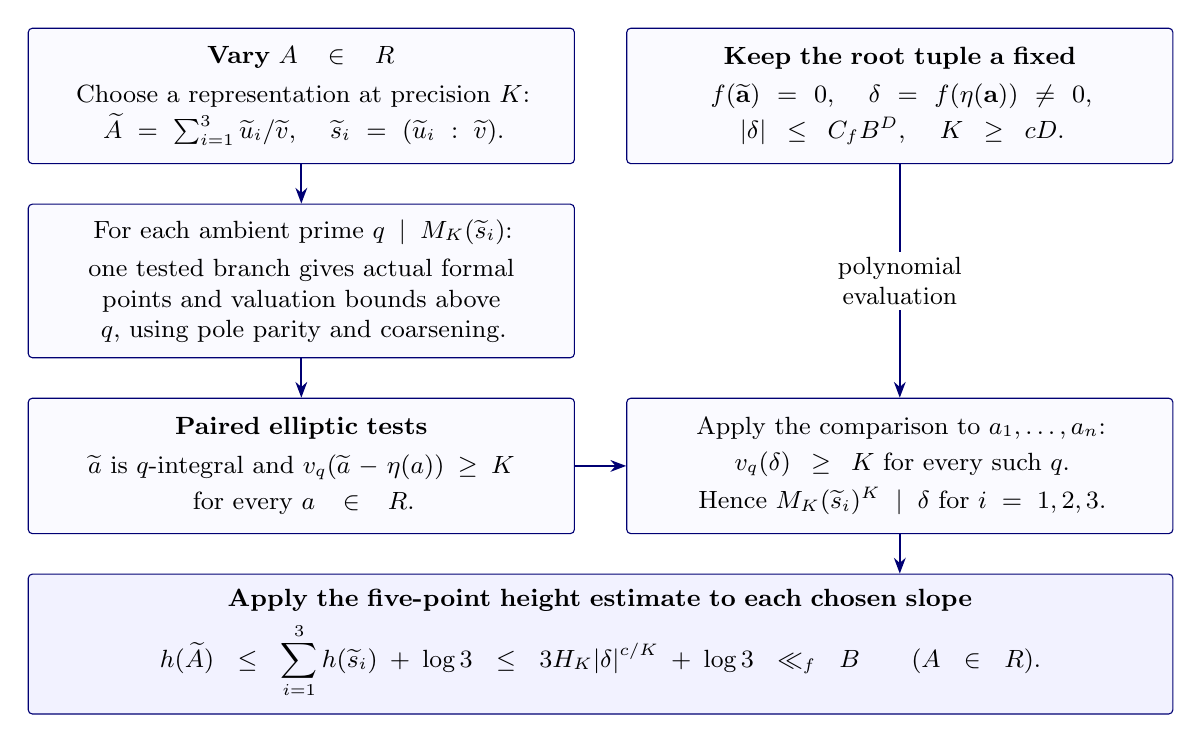
\begin{tikzpicture}[
  box/.style={draw=blue!45!black,fill=blue!2,rounded corners=1.5pt,
              align=center,font=\small,inner sep=5.5pt,text width=6.55cm},
  result/.style={box,text width=14.15cm,fill=blue!5},
  line/.style={-{Stealth[length=2mm]},semithick,draw=blue!45!black}]
\node[box,minimum height=1.72cm] (slopes)
  {\textbf{Vary $A\in R$}\\[3pt]
   Choose a representation at precision $K$:\\[2pt]
   $\widetilde A=\sum_{i=1}^3\widetilde u_i/\widetilde v$,
   \quad $\widetilde s_i=(\widetilde u_i:\widetilde v)$.};
\node[box,minimum height=1.72cm,right=0.65cm of slopes] (root)
  {\textbf{Keep the root tuple $\mathbf a$ fixed}\\[3pt]
   $f(\widetilde{\mathbf a})=0$, \quad
   $\delta=f(\eta(\mathbf a))\ne0$,\\[2pt]
   $|\delta|\le C_f B^D$, \quad $K\ge cD$.};

\node[box,below=0.5cm of slopes] (local)
  {For each ambient prime $q\mid M_K(\widetilde s_i)$:\\[3pt]
   one tested branch gives actual formal points
   and valuation bounds above $q$, using
   pole parity and coarsening.};

\node[box,minimum height=1.72cm,below=0.5cm of local] (comparison)
  {\textbf{Paired elliptic tests}\\[3pt]
   $\widetilde a$ is $q$-integral and
   $v_q(\widetilde a-\eta(a))\ge K$\\[2pt]
   for every $a\in R$.};
\node[box,minimum height=1.72cm,right=0.65cm of comparison] (error)
  {Apply the comparison to $a_1,\ldots,a_n$:\\[2pt]
   $v_q(\delta)\ge K$ for every such $q$.\\[3pt]
   Hence $M_K(\widetilde s_i)^K\mid\delta$
   for $i=1,2,3$.};

\node[result,minimum height=1.62cm,below=0.5cm of comparison,
  xshift=3.8cm] (height)
  {\textbf{Apply the five-point height estimate to each chosen slope}\\[3pt]
   $\displaystyle
   \hgt(\widetilde A)
     \le\sum_{i=1}^3\hgt(\widetilde s_i)+\log3
     \le 3H_K|\delta|^{c/K}+\log3
     \ll_f B\qquad(A\in R).$};

\draw[line] (slopes)--(local);
\draw[line] (local)--(comparison);
\draw[line] (comparison)--(error);
\draw[line] (root)-- node[midway,fill=white,inner sep=2pt,
  font=\small,align=center] {polynomial\\evaluation} (error);
\draw[line] (error.south)--(height.north -| error.south);
\end{tikzpicture}
\caption{The use of one nonzero $\delta$ for every $A\in R$.
All slopes shown come from the representation chosen at the fixed ordinary
precision $K$, and $M_K$ uses the fixed exceptional set for $K$.
The comparison holds for every $a\in R$, so it applies to the fixed root tuple.
The implied constant in the final bound is ordinary and independent of $A$
and $\mathbf a$.}
\label{fig:finite-test-proof}
\end{figure}


For any $A\in R$, take its representation at precision $K$ and
any prime $q$ counted in any $M_K(\widetilde s_i)$.
Proposition~\ref{red:index-congruence} applies to each $a_j$.
Both the embedded coordinates and their integer indices are
\(q\)-integral. Since \(f(\widetilde{\mathbf a})=0\) in the ambient
field and the coefficients of \(f\) are integers, their coordinatewise
congruences give
\begin{equation}\label{red:error-divisibility}
                                  v_q(\delta)\ge K.
\end{equation}
For each fixed slope, \eqref{red:error-divisibility} now holds for
every ambient prime counted by its radical. This is the internal
universal premise in the transfer of the ordinary divisibility fact:
if every prime in a squarefree product divides an integer to order at
least \(K\), then the \(K\)th power of that product divides the integer.
Using the transferred finite-product function gives
\begin{equation}\label{red:radical-divides}
                             M_K(\widetilde s_i)^K\mid\delta.
\end{equation}
The coarsenings may have been chosen externally one prime at a time;
only the universal assertion just established enters this transferred
implication. Although \(A\) and its representation were arbitrary,
the integer \(\delta\) is the same for all of them.

As $\delta\ne0$, \eqref{red:radical-divides} and
\eqref{red:error-bound} give
\[
 M_K(\widetilde s_i)^c
       \le |\delta|^{c/K}
       \le C_f^{c/K}B^{cD/K}\ll_f B.
\]
The height estimate therefore implies
\begin{equation}\label{red:slope-height}
                               \hgt(\widetilde s_i)\ll_f B.
\end{equation}
Since $v\ne0$ and $u_1+u_2+u_3=Av$, the ordinary logarithmic height
inequality for a sum of three numbers, transferred to the ambient
structure, gives
\begin{equation}\label{red:all-ring-height}
 \hgt(\widetilde A)
   =\hgt\!\left(\frac{\widetilde u_1}{\widetilde v}
             +\frac{\widetilde u_2}{\widetilde v}
             +\frac{\widetilde u_3}{\widetilde v}\right)
       \le\sum_{i=1}^3\hgt(\widetilde s_i)+\log3
       \ll_f B \qquad(A\in R).
\end{equation}
The implicit constant is ordinary and independent of $A$ and of the
root tuple. The dependence on $f$ comes only from its degree and
coefficients and the resulting fixed choice of $K$.

For each nonzero \(a_j\), formula
\eqref{red:coordinate-functions} expresses \(x(T_{a_j})\) using
the three ring elements \(x_0(a_j),x_1(a_j),x_2(a_j)\), with
\(x_2(a_j)\ne0\). Applying \eqref{red:all-ring-height} to these
three elements and using the logarithmic height inequalities over the
fixed number field \(F\) gives
\begin{equation}\label{red:elliptic-upper}
                         \hgt(x(\eta(a_j)P))\ll_f B.
\end{equation}
Canonical height on the fixed elliptic curve gives, for ordinary
integer $n\ne0$, and hence for ambient integer indices by transfer,
\begin{equation}\label{red:elliptic-lower}
             \hgt(x(nP))=2\widehat h(P)n^2+O(1),
                         \qquad\widehat h(P)>0;
\end{equation}
see \cite{Silverman2009}. The error term is uniformly bounded for
the fixed curve and point. If $B>1$, choose a maximizing nonzero
index in \eqref{red:B-D}. Equations
\eqref{red:elliptic-upper}--\eqref{red:elliptic-lower} give
\[
                         2\widehat h(P)B^2\le C B+C'
\]
for ordinary constants, so $B$ is bounded by an ordinary constant.
This is also true if $B=1$.

Every element of ${}^*\Z$ in an ordinary finite interval is an
ordinary integer, by transfer of the finite description of that
interval. Thus $\eta(a_j)=n_j\in\Z$ for each $j$.
By additivity and $\eta(1)=1$, $\eta(n_j)=n_j$; injectivity then
gives $a_j=n_j$ in $R$. The relation $f(\mathbf a)=0$ is consequently
an ordinary integer solution. In the case currently under consideration
this also contradicts $\delta\ne0$.
\end{proof}

\begin{proof}[Proof of Theorem~\ref{thm:main}]
Constant polynomials can be decided directly. For nonconstant $f$,
if every finite rational test succeeds,
Proposition~\ref{red:finite-test-success} gives an integer zero. Therefore,
when $f$ has no integer zero, some finite test must fail. Run the
finite-test search and enumeration of integer tuples in parallel,
allocating successive finite steps to each. The enumeration terminates
when a zero exists; the test search terminates when none exists.
Their answers are sound. Rational decidability would therefore give
integer decidability, contradicting the Davis--Putnam--Robinson--Matiyasevich
theorem \cite{DavisPutnamRobinson1961,Matiyasevich1970}.
\end{proof}


\section{An existential condition excluding odd poles}\label{par:section}

We prove Proposition~\ref{par:pole-parity}, used in the finite rational
tests of Section~\ref{sec:reduction}.  It requires a positive existential
condition that holds on all integers and restricts the denominators of any
rational number satisfying it.  Square classes below mean classes in the
multiplicative group modulo squares.

Earlier existential formulas make related valuation information
accessible on restricted sets of primes.  For a fixed global field
\(K\) of characteristic different from \(2\) and a fixed quadratic
extension \(L/K\), Demeyer and Van Geel give an existential formula
which, for nonzero \(x,y\in K\), is equivalent to
\[
 v_{\mathfrak p}(x)\ \text{odd}
 \quad\Longrightarrow\quad
 v_{\mathfrak p}(x/y^2)>0
 \qquad
 \text{for every nonarchimedean prime \(\mathfrak p\) inert in \(L/K\)}.
\]
They also permit a fixed finite union of such inert-prime sets
\cite[Theorem~14 and Corollary~15 in the author version]{DemeyerVanGeel2006}.
Cornelissen and Zahidi use related odd-valuation predicates in their
elliptic-divisibility approach
\cite[Sections~3.3 and~3.11]{CornelissenZahidi2007}.
The existential definitions of Demeyer and Van Geel control the
chosen inert primes.
Proposition~\ref{par:pole-parity} instead supplies the stated
one-sided restriction outside a fixed finite exceptional set.

We first define a formula from finite multiplier lists and prove the
pole restriction. We then choose the lists once and for all and prove
integer completeness by realizing the same square class on two elliptic
curves.

\subsection{The formula and the pole restriction}

For now, let $\mathcal M\subset\Q^\times$ be a finite nonempty list,
and for each $m\in\mathcal M$ let $\mathcal D_m\subset\Q^\times$
be a finite nonempty list. The construction below associates a formula
$\Phi$ to these lists. Let $S_1$ be a finite set containing $2$, $3$,
and the supports of every member of all the lists. We will make one
fixed choice of the lists in the next subsection.

For $l\in\Q^\times$, write
\begin{equation}\label{par:curve}
 E_l:\quad y^2=x(x-l)(x+3l).
\end{equation}
The three roots are distinct, so this is an elliptic curve with its
point at infinity $O$ as origin. Define $\Phi(b)$ to hold if $b=0$,
or if $b\ne0$ and, for some $m\in\mathcal M$, $m_d\in\mathcal D_m$,
and $t,e\in\Q$, the following conditions hold:
\begin{equation}\label{par:auxiliary-functions}
 d=m_db,\qquad b'=mb,\qquad
 U=b\frac{1-dt^2}{1+dt^2},\qquad H'=b'(b'-U^2),
\end{equation}
\[
 1+dt^2\ne0,\qquad eH'\ne0,
\]
and each of $E_e$ and $E_{eH'}$ has a rational point whose
$x$-coordinate belongs to $b'\Q^{\times2}$.

For each fixed choice of the lists, this is a positive existential
formula. The choices of multipliers are finite disjunctions. A nonzero
condition $a\ne0$ is the existential equation $az=1$; the condition on
$x$ is expressed by $x=b'z^2$ with $z\ne0$. Introduce $U$ as a variable
and multiply its defining equality by $1+dt^2$. All remaining conditions
are polynomial equalities with fixed rational coefficients, which can be
cleared to integer coefficients.

\begin{lemma}\label{par:soundness}
For any finite lists as above, if $b\in\Q^\times$ satisfies $\Phi(b)$
and $q\notin S_1$, then $v_q(b)<0$ implies $v_q(b)\in2\Z$.
\end{lemma}

\begin{proof}
Suppose that $q\notin S_1$, that witnesses for $\Phi(b)$ have been
chosen, and that $k=v_q(b)<0$ is odd. The multipliers are $q$-adic
units, so $v_q(d)=v_q(b')=k$. If $t=0$, then $U=b$. If $t\ne0$,
the valuation $v_q(dt^2)=k+2v_q(t)$ is odd and hence nonzero.
When this valuation is positive, both $1-dt^2$ and $1+dt^2$ are
units. When it is negative, both have valuation $v_q(dt^2)$.
In either case $v_q(U)=k$. Since $2k<k$,
\[
 v_q(b'-U^2)=2k,\qquad v_q(H')=3k.
\]
Consequently $v_q(e)$ and $v_q(eH')$ have opposite parities. Let
$l$ be the one of these two parameters whose valuation is even,
say $v_q(l)=2a$. Replacing
\[
 l=q^{2a}L,\qquad x=q^{2a}X,\qquad y=q^{3a}Y
\]
gives $Y^2=X(X-L)(X+3L)$ with $L\in\Z_q^\times$ and does not
change the square class of $x$.

Every nonzero $X$ on this unit-parameter curve has even valuation.
Indeed, if $v_q(X)<0$, all three factors have valuation $v_q(X)$,
so the right side has valuation $3v_q(X)$. If $v_q(X)>0$, the
other two factors are units because $q\ne3$, so its valuation is
$v_q(X)$. In both cases this valuation must be even. The case
$v_q(X)=0$ already has the desired parity. This contradicts
$x\in b'\Q_q^{\times2}$, since $v_q(b')=k$ is odd.
\end{proof}


\subsection{Preparing integer witnesses}

We now choose the multiplier lists so that the formula also holds on
every integer. These lists will be fixed independently of the input
$b$. Choose a finite list $\mathcal M\subset\Q^\times$ with the
following property: for every $b\in\Q^\times$, some $m\in\mathcal M$
makes
\begin{equation}\label{par:b-prime-choices}
 b'=mb>0,\qquad b'\in\Q_2^{\times2},\qquad
 b'\in\text{the unit nonsquare class of }\Q_3^\times.
\end{equation}
Here the last condition means that $b'$ has even $3$-adic valuation
and nonsquare unit part. Such a list exists because
$\R^\times/\R^{\times2}$, $\Q_2^\times/\Q_2^{\times2}$, and
$\Q_3^\times/\Q_3^{\times2}$ are finite, their classes are open,
and weak approximation supplies a rational representative for each
specified finite tuple of classes. For each $m\in\mathcal M$, set
\[
 S(m)=\{2,3\}\cup\operatorname{Supp}(m).
\]
The same argument gives a finite list
$\mathcal D_m\subset\Q^\times$ such that, for any $b\ne0$, some
$m_d\in\mathcal D_m$ makes
\begin{equation}\label{par:d-choices}
 d=m_db>0,\qquad d\in\Q_q^{\times2}\quad(q\in S(m)).
\end{equation}
Use these fixed lists in $\Phi$, and fix $S_1$ containing $2$, $3$,
and all their supports as above. The normalizations
\eqref{par:b-prime-choices}--\eqref{par:d-choices} are used only to
select entries $m,m_d$ for an integer input; they are not additional
conjuncts of $\Phi$. Lemma~\ref{par:soundness} already proves the pole
restriction for this choice.

Fix $b\in\Z\setminus\{0\}$ and choose $m,m_d$ so that
\eqref{par:b-prime-choices} and \eqref{par:d-choices} hold.
We choose $t$ to serve two purposes. The value $U$ should be small at
the places where $d$ was made a local square, while at primes outside
$S(m)$ where $v_q(b')$ is odd it should retain the valuation of $b$.
These properties will make $H'$ a local square at every prime where
$v_q(b')$ is odd, and $b'$ a local square at every prime where
$v_q(H')$ is odd.

At the real place and at every $q\in S(m)$, choose a local solution
of $dt^2=1$. As $t$ tends to this solution, the rational function
$U$ tends to zero: its denominator tends to the nonzero number $2$.
Thus, in sufficiently small neighborhoods, $H'>0$ at the real place,
and
\[
 H'=b'^2\left(1-\frac{U^2}{b'}\right)\in\Q_q^{\times2}
 \quad(q\in S(m)),
\]
by openness of the local square subgroup. At every
$q\in\operatorname{Supp}(m_d)\setminus S(m)$, require $t$ to be
so small that $v_q(dt^2)>0$. Weak approximation satisfies all these
conditions simultaneously with a rational $t$. In particular
$1+dt^2\ne0$ and $H'>0$.

Let $\beta,\theta$ be the unique positive squarefree integers
representing the square classes of $b',H'$, and let
\[
 B=\operatorname{Supp}(\beta),\qquad
 J=\operatorname{Supp}(\theta).
\]

\begin{lemma}\label{par:cross-squares}
The sets $B,J$ are disjoint and avoid $2,3$. Moreover,
\begin{equation}\label{par:mutual-squares}
 \theta\in\Q_q^{\times2}\quad(q\in B),\qquad
 \beta\in\Q_q^{\times2}\quad(q\in J).
\end{equation}
Both $\beta$ and $\theta$ are squares in $\Q_2^\times$; at $3$,
$\theta$ is a square and $\beta$ is a unit nonsquare. In particular
$B\ne\varnothing$.
\end{lemma}

\begin{proof}
The assertions at $2,3$ follow from the choices already made and
are unchanged on replacing numbers by square-class representatives.
At a prime $q\in B\cap S(m)$, $H'$ is a local square by construction.
Now suppose $q\in B\setminus S(m)$. Since $m$ is a unit at $q$ and
$b$ is an integer, $v_q(b)=v_q(b')$ is a positive odd integer.
If $q\notin\operatorname{Supp}(m_d)$ and $t\ne0$, then
$v_q(dt^2)=v_q(b)+2v_q(t)$ is odd and nonzero, and the quotient
$(1-dt^2)/(1+dt^2)$ is a unit, just as in
Lemma~\ref{par:soundness}. For $t=0$ this quotient is $1$.
If instead $q\in\operatorname{Supp}(m_d)$, our additional smallness
condition on $t$ also makes it a unit. Hence $v_q(U)=v_q(b)$, and
\[
 v_q(U^2/b')=v_q(b)>0.
\]
As $q$ is odd, $1-U^2/b'$ is a local square. The displayed formula
for $H'$ proves the first assertion of \eqref{par:mutual-squares},
and also proves $B\cap J=\varnothing$.

For the converse assertion, let $q\in J$. Such a prime is outside
$S(m)$, since $H'$ is square there, and $v_q(b')$ is even because
$q\notin B$. If $U=0$, then $H'=b'^2$ and there is no such prime,
so suppose $U\ne0$. Put
\[
 \alpha=v_q(b'),\qquad \gamma=2v_q(U).
\]
Both are even. If $\alpha\ne\gamma$, then
$v_q(b'-U^2)=\min(\alpha,\gamma)$ is even, contrary to
the oddness of $v_q(H')$. Therefore $\alpha=\gamma$.
Since $v_q(H')=\alpha+v_q(b'-U^2)$ is odd, cancellation is
strict: $v_q(b'-U^2)>\alpha$. Thus
$b'/U^2\in1+q\Z_q$, a square in $\Q_q^\times$, proving that
$\beta$ is square there. This argument also covers possible
denominators in $t$ or $U$. Finally $\beta$ cannot be $1$, since
its class at $3$ is nonsquare.
\end{proof}


Write $H'=\theta c^2$ with $c\in\Q^\times$. For every $n\in\Q^\times$
the isomorphism
\begin{equation}\label{par:twist-scaling}
 E_{n\theta}\longrightarrow E_{nH'},\qquad
 (x,y)\longmapsto(c^2x,c^3y)
\end{equation}
preserves $x$-coordinate square classes. Thus, taking $e=n$ in the
formula, it remains to find one $n$ for which both $E_n$ and
$E_{n\theta}$ have a rational point with nonzero $x$-coordinate of class
$\beta$, the class of $b'$. We first give a criterion for one parameter
$l$, and then construct a single $n$ for which it applies to both twists.

\subsection{A criterion for one twist}

We recall the exact part of full two-descent that we use; see
\cite[Chapter~X, Proposition~1.4, p.~315]{Silverman2009}. For a split
separable cubic $y^2=\prod_{i=1}^3(x-e_i)$ over a field $k$ of
characteristic zero, choosing two roots identifies
$H^1(k,E[2])$ with $(k^\times/k^{\times2})^2$. In the coordinate
corresponding to $e_i$, the Kummer map takes a point to the class
of $x-e_i$; at $(e_i,0)$ the value is replaced by
$\prod_{j\ne i}(e_i-e_j)$, and at $O$ it is $1$.
The Kummer map is an injection of $E(k)/2E(k)$ into this group.
The group $\Sel_2(E/\Q)$ is the subgroup of rational pairs lying
in the Kummer image at every completion. The standard Selmer exact
sequence \cite[Chapter~X, Theorem~4.2, p.~333]{Silverman2009} is
\begin{equation}\label{par:selmer-exact-sequence}
 0\longrightarrow E(\Q)/2E(\Q)
 \longrightarrow\Sel_2(E/\Q)
 \longrightarrow\Sha(E/\Q)[2]\longrightarrow0.
\end{equation}


We use the coordinates $(x+3l,x-l)$ for $E_l$. For a finite rational
point $T$ with $x(T)\notin\{0,l,-3l\}$, the curve equation gives
\[
             [x(T)]=[x(T)+3l]\,[x(T)-l].
\]
Consequently, if the class $(\beta,1)$ is represented by a rational
point and is distinct from the classes of all four rational two-torsion
points, that point has the required nonzero $x$-coordinate class $\beta$.
The next calculation identifies conditions that make $(\beta,1)$ the
one additional Selmer direction beyond rational two-torsion.

For the Selmer graph-matrix viewpoint underlying this calculation, see
Monsky's appendix to Heath-Brown \cite[Appendix, pp.~365--370]{HeathBrown1994}.
The matrix and simultaneous rank calculations below adapt that viewpoint
to the present curve family.

At the primes dividing $l$, the local square conditions will be recorded
by binary residue symbols. For an odd prime $q$ and a $q$-adic unit $a$,
write $[a/q]\in\F_2$ for the nonsquare bit: it is $0$ for a square
residue and $1$ for a nonsquare residue. For a finite set $Q$ of distinct
primes different from $2,3$, indexed by $i$, and a vector $w\in\F_2^Q$,
write $D_w$ for the diagonal matrix with diagonal $w$. Put
\begin{equation}\label{par:matrices}
 s_i=[-1/q_i],\qquad \lambda_i=[3/q_i],\qquad
 (Ku)_i=\sum_{j\ne i}[q_j/q_i](u_j+u_i),\qquad N=K+D_s.
\end{equation}
All matrices and vectors in this calculation are over $\F_2$. Write
$\mathbf1$ for the all-ones vector and $\mathbf1_B$ for the indicator
of $B$ in $Q$. Quadratic reciprocity gives
\begin{equation}\label{par:reciprocity-matrix}
 K+K^{\mathsf t}=ss^{\mathsf t}+D_s.
\end{equation}
In particular, if $s^{\mathsf t}\mathbf1=1$, then
\begin{equation}\label{par:matrix-null-vectors}
 K\mathbf1=K^{\mathsf t}\mathbf1=0,
 \qquad N=K^{\mathsf t}+ss^{\mathsf t}.
\end{equation}

The family \(y^2=x(x-n)(x+3n)\) also occurs in the study of
\(\pi/3\)- and \(2\pi/3\)-congruent numbers.  Mokrani adapted
Monsky matrices to these families \cite{Mokrani2020}.  For this
family, Wei and Guo give a two-Selmer matrix formulation and write
the same quadratic-reciprocity identity for the associated R\'edei
matrix as \eqref{par:reciprocity-matrix}
\cite[Section~4 and Theorem~6.2]{WeiGuo2022}.  The simultaneous
kernel conditions for the two twists required here are constructed
below.

\begin{lemma}\label{par:descent}
Let $l>0$ be squarefree, prime to $6$, with
$l\equiv3\pmod4$ and $l\equiv2\pmod3$. Suppose that its support
$Q$ contains the nonempty set $B$ of Lemma~\ref{par:cross-squares}
and a prime outside $B$, and suppose that
\begin{equation}\label{par:matrix-target}
 \ker K=\langle\mathbf1,\mathbf1_B\rangle,
 \qquad \lambda\notin\operatorname{im}K.
\end{equation}
Then
\[
 \dim_{\F_2}\Sel_2(E_l/\Q)=3,
\]
and $(\beta,1)$ is a Selmer class outside the subgroup of rational
two-torsion classes, in Kummer coordinates $(x+3l,x-l)$.
\end{lemma}

\begin{proof}
In the stated coordinates, the points $(l,0)$ and $(-3l,0)$ have
classes
\begin{equation}\label{par:torsion-classes}
 \tau_1=(l,1),\qquad \tau_2=(3,-l),
\end{equation}
respectively. For example, the replacement coordinate at $(l,0)$
is $(l+3l)l=4l^2$, and the replacement at $(-3l,0)$ is
$(-3l)(-4l)=12l^2$. These two classes are independent globally:
$l$ is nonsquare, and the second coordinate of $\tau_2$ is negative.

We first bound the Selmer group using necessary local conditions.
Afterward we verify that $(\beta,1)$ lies in the actual local Kummer
image everywhere. For any odd prime $q$, the group
$E_l(\Q_q)/2E_l(\Q_q)$ has order four. To see this, choose an
open formal subgroup $H$ on which multiplication by $2$ is an
isomorphism. The quotient $G=E_l(\Q_q)/H$ is finite, and
$E_l(\Q_q)/2E_l(\Q_q)\simeq G/2G$. Moreover
$E_l(\Q_q)[2]\simeq G[2]$: injectivity follows from $H[2]=0$,
and a lift of any element of $G[2]$ can be corrected by an element
of $H$, using the surjectivity of multiplication by $2$ on $H$.
Finally $|G/2G|=|G[2]|=4$.

At an odd prime $q\nmid3l$, the roots are integral and pairwise
distinct modulo $q$. If $v_q(x)<0$, all three factors have that
valuation, which must be even. If $x$ is integral, at most one
factor has positive valuation, and that valuation must be even.
The replacement classes at the roots are units as well. Hence
the local Kummer image is contained in the subgroup of pairs
having even coordinate valuations. This unramified subgroup has
order four, so the containment is equality.

At a support prime $q_i\mid l$, the valuation pairs of $\tau_1$
and $\tau_2$ are $(1,0)$ and $(0,1)$ modulo $2$; therefore they
generate the entire local image, again by its order four. At $3$,
$l$ is a unit nonsquare and $-l$ is a square. Thus $\tau_1$
and $\tau_2$ have independent first-coordinate classes and square
second coordinates. The local image at $3$ is consequently
\begin{equation}\label{par:local-three}
 (\Q_3^\times/\Q_3^{\times2})\times\{1\}.
\end{equation}

At $2$ we need the necessary condition that both Kummer coordinates
have even valuation. For a point away from the roots with
$v_2(x)<0$, all three factors have valuation $v_2(x)$, so that
valuation is even. If $x$ is integral and even, $x+3l$ and $x-l$
are units. Suppose $x$ is odd. If $x-l=2u$ with $u$ odd, then
\[
 (y/2)^2=(l+2u)u(u+2l)\equiv l\pmod8.
\]
The right side is an odd unit congruent to $3$ or $7$ modulo $8$,
which is impossible for a square. In every remaining nonroot
case, $v_2(x-l)\ge2$ and $v_2(x+3l)\ge2$. Their difference is
$4l$, so their minimum valuation is $2$. Since $x$ is a unit,
their valuation sum is even, and hence both valuations are even.
The root and identity classes also have even valuations, as follows
from \eqref{par:torsion-classes}. This establishes the claimed
necessary condition at $2$; no sufficiency is being asserted.

At the real place the first coordinate is always positive. Indeed,
for a nonroot real point the allowable $x$ intervals are
$(-3l,0)$ and $(l,\infty)$, and the replacement first coordinates
at the roots are positive as well. The sign of the second coordinate
therefore gives a homomorphism from the Selmer group to
$\{\pm1\}$, and it is surjective because of $\tau_2$. Its kernel,
the classes with both coordinates positive, has index two.
Every class in this kernel has a unique representative of the form
\begin{equation}\label{par:normalized-pair}
 \left(3^\delta\prod_iq_i^{u_i},\ \prod_iq_i^{v_i}\right),
 \qquad \delta\in\F_2,\quad u,v\in\F_2^Q.
\end{equation}
Here the good-prime restrictions and the even valuations at $2$
exclude every other prime, and \eqref{par:local-three} excludes
$3$ from the second coordinate.

At $q_i$, compare \eqref{par:normalized-pair} with the local
torsion class
\[
 \tau_1^{u_i}\tau_2^{v_i}
   =(l^{u_i}3^{v_i},(-l)^{v_i}).
\]
The coordinate valuations already agree modulo $2$. Requiring
the resulting unit quotients to be squares gives exactly
\begin{equation}\label{par:selmer-matrix-equations}
 Ku+D_\lambda v=\delta\lambda,\qquad Nv=0.
\end{equation}
For example the first unit quotient has nonsquare bit
$\sum_{j\ne i}[q_j/q_i](u_j+u_i)+(\delta+v_i)\lambda_i$;
the second has bit $(Kv)_i+s_iv_i$. The requirement that the
second coordinate be square at $3$ adds
\begin{equation}\label{par:selmer-three-equation}
 (\lambda+s)^{\mathsf t}v=0,
\end{equation}
using $[q_i/3]=\lambda_i+s_i$.

The residue assumptions imply
$s^{\mathsf t}\mathbf1=1$ and $\lambda^{\mathsf t}\mathbf1=0$.
Equations \eqref{par:matrix-null-vectors} give
\begin{equation}\label{par:kernel-N}
 \ker N=\ker K^{\mathsf t}\cap s^\perp.
\end{equation}
Indeed, left multiplying $Nv=0$ by $\mathbf1^{\mathsf t}$
gives $s^{\mathsf t}v=0$, and the identity
$N=K^{\mathsf t}+ss^{\mathsf t}$ then gives the claim in both
directions. By \eqref{par:matrix-target}, $\ker K^{\mathsf t}$
has dimension two. It contains $\mathbf1$, on which
$s^{\mathsf t}$ is nonzero, so \eqref{par:kernel-N} is a line.
The functional $\lambda^{\mathsf t}$ is nonzero on
$\ker K^{\mathsf t}$ because
$\lambda\notin\operatorname{im}K=(\ker K^{\mathsf t})^\perp$.
Since it vanishes on $\mathbf1$, it is nonzero on the complementary
line \eqref{par:kernel-N}. Equations
\eqref{par:selmer-three-equation} and \eqref{par:kernel-N}
therefore force $v=0$. The first equation in
\eqref{par:selmer-matrix-equations} now gives
$Ku=\delta\lambda$, so $\delta=0$ and
$u\in\ker K=\langle\mathbf1,\mathbf1_B\rangle$.
There are at most four sign-normalized classes, and hence at
most eight Selmer classes.

For equality, we verify that
\[
 \gamma=(\beta,1)
\]
is an actual local Kummer class everywhere. At $2$ and at the real
place it is the identity class, since $\beta$ is a positive local
square. At $3$ it is $\tau_1$, since $\beta$ and $l$ are both
unit nonsquares. At $q_i\mid l$, take $u=\mathbf1_B$ and $v=0$:
the comparison with $\tau_1^{u_i}$ has square coordinate quotients
precisely because $K\mathbf1_B=0$. At every other finite odd
prime it is unramified, so lies in the local image already
described. This proves $\gamma\in\Sel_2(E_l/\Q)$.
It is neither the identity nor $\tau_1$: $B$ is nonempty, and
$l$ has a prime factor outside $B$. It cannot equal $\tau_2$ or
$\tau_1\tau_2$, whose second coordinates are negative. Thus
$\tau_1,\tau_2,\gamma$ are three independent Selmer classes,
and the upper bound is attained.
\end{proof}


It remains to realize this particular Selmer class by a rational point.
The consequence we use from Theorem~1.1 of \cite{PointwiseTwoConverse}
is the following: an elliptic curve $C/\Q$ with $C(\Q)[2]\ne0$ and
$\corank_{\Z_2}\Sel_{2^\infty}(C/\Q)\in\{0,1\}$ has finite
$\Sha(C/\Q)$. The next proof verifies the full Selmer-corank hypothesis
before applying it.

\begin{lemma}\label{par:global-point}
Under the hypotheses of Lemma~\ref{par:descent}, the curve $E_l$
has a rational point with nonzero $x$-coordinate in
$\beta\Q^{\times2}$.
\end{lemma}

\begin{proof}
Put $r=\rank E_l(\Q)$. Since $E_l$ has full rational two-torsion,
the Kummer sequence \eqref{par:selmer-exact-sequence} and
Lemma~\ref{par:descent} imply
\begin{equation}\label{par:rank-sha}
 r+\dim_{\F_2}\Sha(E_l/\Q)[2]=1.
\end{equation}
This also controls the full $2$-primary Selmer group before any
finiteness conclusion. The usual exact sequence is
\[
 0\longrightarrow E_l(\Q)\otimes\Q_2/\Z_2
 \longrightarrow\Sel_{2^\infty}(E_l/\Q)
 \longrightarrow\Sha(E_l/\Q)[2^\infty]\longrightarrow0.
\]
These are cofinitely generated $\Z_2$-modules. If the last group
has corank $t$, its structure is
$(\Q_2/\Z_2)^t\oplus F$ with $F$ finite, so
$t\le\dim_{\F_2}\Sha(E_l/\Q)[2]$. It follows from
\eqref{par:rank-sha} that
\[
 0\le\corank_{\Z_2}\Sel_{2^\infty}(E_l/\Q)=r+t\le1.
\]
The curve has nonzero rational two-torsion, so
\cite[Theorem~1.1]{PointwiseTwoConverse} now applies and proves
that $\Sha(E_l/\Q)$ is finite.

The Cassels--Tate pairing on this finite group is perfect and
alternating. Alternation here uses the principal polarization
represented by the rational divisor $(O)$; see
\cite{Cassels1962}; see also
\cite[Section~1 and Corollary~9]{PoonenStoll1999}. For completeness,
an alternating perfect pairing on a finite abelian $2$-group
forces an even number of cyclic factors. Choose an element $x$
of maximal order $2^a$. Perfection supplies $y$ whose pairing
with $x$ has exact order $2^a$. The subgroup generated by $x,y$
is a nondegenerate copy of $(\Z/2^a\Z)^2$, and the whole group
is its direct sum with its orthogonal complement. Induction gives
a decomposition into such paired cyclic factors. Hence
\[
 \dim_{\F_2}\Sha(E_l/\Q)[2]\quad\text{is even}.
\]
This conclusion uses the perfect pairing on the full finite
$2$-primary group; its restriction to the subgroup killed by $2$
need not be perfect. Equation~\eqref{par:rank-sha} therefore gives
$\Sha(E_l/\Q)[2]=0$ and $r=1$.

The Kummer sequence now shows that $\gamma=(\beta,1)$ is the
class of a rational point $T$. By Lemma~\ref{par:descent} its class
differs from all four two-torsion point classes. Thus $T$ is finite
and none of $x(T)$, $x(T)-l$, $x(T)+3l$ is zero. The curve equation
gives, modulo squares,
\[
 [x(T)]=[x(T)+3l]\,[x(T)-l]=\beta,
\]
as required.
\end{proof}


\begin{remark}
The unrestricted $2$-converse \cite[Theorem~1.1]{UnrestrictedTwoConverse}
can replace the pointwise theorem in the preceding proof. It gives
finiteness of the whole $\Sha(E_l/\Q)$ from the same full Selmer-corank
bound, without any rational-two-torsion hypothesis.
\end{remark}

\subsection{One parameter for both twists}

The criterion is now a condition on the prime support of one twist.
We construct a single positive squarefree $n$ for which it holds both
on the support of $n$ and on that of $n\theta$. The mutual local-square
relations from Lemma~\ref{par:cross-squares} are what allow the second
support to be added without disturbing the first construction.

\begin{lemma}\label{par:simultaneous-matrices}
For $\beta,\theta,B,J$ as in Lemma~\ref{par:cross-squares}, there is
a positive squarefree integer $n$, prime to $6\theta$, whose support
$P$ contains $B$ and at least one auxiliary prime outside $B$, such
that the following statements hold for both $l=n$ and $l=n\theta$.
The number $l$ satisfies $l\equiv3\pmod4$ and $l\equiv2\pmod3$.
On its prime support $Q=P$ or $Q=P\cup J$, the matrices
\eqref{par:matrices} satisfy \eqref{par:matrix-target}.
\end{lemma}

\begin{proof}
Since $\beta,\theta$ are odd squares at $2$, their products of
$(-1)$-symbols are $1$. At $3$, reciprocity gives
$[q/3]=[3/q]+[-1/q]=\lambda_q+s_q$. Consequently
\begin{equation}\label{par:fixed-symbol-sums}
 \sum_{i\in B}s_i=\sum_{j\in J}s_j=0,\qquad
 \sum_{i\in B}\lambda_i=1,\qquad
 \sum_{j\in J}\lambda_j=0.
\end{equation}
The fixed $B$--$J$ symbols need not vanish individually. Their
row sums, however, satisfy
\begin{equation}\label{par:cross-symbol-sums}
 \sum_{j\in J}[q_j/q_i]=0\quad(i\in B),\qquad
 \sum_{i\in B}[q_i/q_j]=0\quad(j\in J),
\end{equation}
by \eqref{par:mutual-squares}.

Introduce one auxiliary prime $q_0$ of type
$(s_0,\lambda_0)=(1,1)$, and a set $I$ of $|B|-1$ auxiliary
primes of type $(0,0)$. These types can be imposed by the residue
classes $7$ and $1$ modulo $12$, respectively. We first prescribe
all required Legendre symbols abstractly, and realize them by actual
primes at the end. Until then, each unchosen symbol is a bit whose reverse
is constrained by quadratic reciprocity; the matrix reciprocity identity
therefore holds for every completion of these choices. On each of the sets
\[
 Q_0=B\cup I\cup\{q_0\},\qquad Q_1=Q_0\cup J,
\]
the total $s$-sum is $1$ and the total $\lambda$-sum is $0$.
The former gives $l\equiv3\pmod4$, while the sum of $s+\lambda$
gives $l\equiv2\pmod3$ for the corresponding prime product.

We first show that, subject to $K\mathbf1_B=0$, both matrix targets follow
from one nonsingularity condition. Fix $b_*\in B$ and let $a$ have entries
$1$ at $q_0,b_*$ and $0$ elsewhere. Thus
\[
 a^{\mathsf t}\mathbf1=0,\qquad
 a^{\mathsf t}\mathbf1_B=1.
\]
We shall impose $K\mathbf1_B=0$ on both supports. Assuming this condition
for the moment, set $K^\#=K+\lambda a^{\mathsf t}$. The total symbol
sums and \eqref{par:matrix-null-vectors} show that $K^\#$ kills
$\mathbf1$ on both sides, and
\begin{equation}\label{par:sharp-B}
 K^\#\mathbf1_B=\lambda.
\end{equation}
Put
\[
 T=\operatorname{Id}-\mathbf1_Ba^{\mathsf t}.
\]
This is a projection onto $a^\perp$, with kernel
$\langle\mathbf1_B\rangle$, and it fixes $\mathbf1$. By
\eqref{par:sharp-B},
\begin{equation}\label{par:projection-factorization}
 K=K^\#T.
\end{equation}
Suppose that $\ker K^\#=\langle\mathbf1\rangle$. If $Kx=0$, then
$Tx=c\mathbf1$, so
$x=c\mathbf1+(a^{\mathsf t}x)\mathbf1_B$; the converse follows from
$K\mathbf1=K\mathbf1_B=0$. This gives the required kernel of $K$.
If $Kx=\lambda$, put $y=Tx$. Then $a^{\mathsf t}y=0$ and
$K^\#(y-\mathbf1_B)=0$, so
$y-\mathbf1_B\in\langle\mathbf1\rangle$. Applying $a^{\mathsf t}$
would give $-1=0$, a contradiction. Thus $\lambda\notin\operatorname{im}K$.

For either support, let $M$ be the matrix obtained from $K^\#$ by
deleting the $q_0$ row and column. It is enough to make $M$ nonsingular.
Indeed, if $K^\#x=0$, subtract $x_{q_0}\mathbf1$ from $x$. The resulting
vector still lies in the kernel, has zero $q_0$ coordinate, and its
remaining coordinates are killed by $M$. Nonsingularity makes that
vector zero, proving $\ker K^\#=\langle\mathbf1\rangle$. We therefore
have two tasks for the symbol choices: impose $K\mathbf1_B=0$ and make
these deleted matrices nonsingular on both supports.

For the smaller support, let $C$ be a $B$-by-$I$ matrix whose columns
are a basis of the even-sum hyperplane
\[
 \{x\in\F_2^B:\mathbf1_B^{\mathsf t}x=0\}.
\]
These columns will form the off-diagonal block of the deleted matrix.
When $|B|=1$, $C$ is the empty matrix. Prescribe
$[q_i/q_b]=[q_b/q_i]=C_{bi}$ for $b\in B,i\in I$.
Every other off-diagonal symbol incident with $I$ is set to zero.
Prescribe
\[
 [q_0/q_b]=\sum_{i\in I}C_{bi}\qquad(b\in B),
\]
and obtain reverse symbols by reciprocity. In particular
$[q_b/q_0]=[q_0/q_b]+s_b$. The $q_0$--$J$ symbols remain free.

These prescriptions ensure $K\mathbf1_B=0$ on both supports.
At a $B$ row, the terms from $I$ and $q_0$ cancel, and the sum
from $J$, when present, is zero by \eqref{par:cross-symbol-sums}.
At an $I$ row the sum is a column sum of $C$, hence zero. At the
$q_0$ row it is the sum of all entries of $C$ plus $\sum_B s_b$,
again zero. At a $J$ row it is zero by the second equality in
\eqref{par:cross-symbol-sums}. It therefore remains to make the deleted
matrices nonsingular.

On $Q_0$, the deleted matrix has the form
\begin{equation}\label{par:block}
 M_0=\begin{pmatrix}A&C\\ C^{\mathsf t}&0\end{pmatrix},
 \qquad \mathbf1_B^{\mathsf t}A\mathbf1_B=1.
\end{equation}
The equality follows from \eqref{par:sharp-B} and
$\sum_B\lambda_b=1$. The lower right block is zero since the
only potentially nonzero symbols incident with $I$ are in $C$,
whose column sums vanish. The added matrix $\lambda a^{\mathsf t}$
changes neither off-diagonal block, because $a$ and $\lambda$
both vanish on $I$. No symmetry of $A$ is required.

To prove $M_0$ nonsingular, let $M_0(x,y)^{\mathsf t}=0$.
The second block equation says $C^{\mathsf t}x=0$. Since the
columns of $C$ span the even-sum hyperplane, its annihilator is
$\langle\mathbf1_B\rangle$; hence $x=c\mathbf1_B$.
Left multiplying the first block equation
$cA\mathbf1_B+Cy=0$ by $\mathbf1_B^{\mathsf t}$ gives $c=0$
by \eqref{par:block}. The injectivity of $C$ then gives $y=0$.
This proof applies also when $|B|$ is even; when $|B|=1$ it says
simply that $M_0=(1)$.

On adding $J$, the $B,I$ block of the deleted matrix stays equal to
$M_0$. Indeed, the only possible changes to its diagonal are the
$B$--$J$ row sums, which vanish by \eqref{par:cross-symbol-sums}; all
$I$--$J$ symbols were set to zero. Now varying the bit $[q_0/q_j]$ for
one $j\in J$ also varies its reverse by the same bit, as their
reciprocity discrepancy is fixed. After deleting the $q_0$ row and
column, the only surviving change is a toggle of the $j$-th diagonal
entry. Thus these choices independently toggle the $J$-diagonal entries
of the enlarged matrix. Its determinant is a multilinear polynomial
in these bits whose coefficient of their full product is $\det M_0=1$.
A nonzero multilinear polynomial over $\F_2$ cannot vanish at every
point of the Boolean cube: this follows by induction on the number of
variables, writing it as $f_0+Xf_1$. Hence some choice makes the enlarged
matrix nonsingular. If $J$ is empty, the smaller-support calculation
already suffices. The chosen bits do not affect the smaller matrix.

The deleted matrices are now nonsingular on both supports, so the
preceding reduction proves \eqref{par:matrix-target} on both.
Finally realize the prescribed symbols. Choose the auxiliary primes
successively. At each step, specify the type modulo $12$ and the
Legendre symbols modulo every already fixed prime in $B\cup J$
or among the earlier auxiliary primes. Each symbol can be imposed
by a nonzero residue modulo that prime; reverse symbols are
consistent by the prescribed reciprocity rule. The Chinese
remainder theorem gives a reduced residue class, and Dirichlet's
theorem supplies infinitely many primes in it. Excluding the
finitely many previously used primes causes no difficulty.
The resulting product
$n=\prod_{q\in B\cup I\cup\{q_0\}}q$ has all the asserted
properties.
\end{proof}

\begin{proof}[Completion of the proof of Proposition~\ref{par:pole-parity}]
The value $b=0$ satisfies $\Phi$ by definition. For a nonzero integer
$b$, make the local choices preceding Lemma~\ref{par:cross-squares} and choose
$n$ by Lemma~\ref{par:simultaneous-matrices}. Both $l=n$ and
$l=n\theta$ satisfy the hypotheses of Lemma~\ref{par:global-point}, so
each curve has a point with nonzero $x$-coordinate of class $\beta$,
which is also the class of $b'$. The isomorphism
\eqref{par:twist-scaling} sends the point on $E_{n\theta}$ to one on
$E_{nH'}$ with the same $x$-coordinate square class. Taking $e=n$
gives the two points required in the definition of $\Phi$, on $E_e$
and $E_{eH'}$. This proves integer completeness, while
Lemma~\ref{par:soundness} proves the asserted pole restriction.
\end{proof}

\section{A height bound from odd contact with five points}\label{hei:section}

We prove Theorem~\ref{hei:height}, whose contact radical supplies the
primes used in Section~\ref{sec:reduction}.  For
\(s\in\mathbf P^1(\Q)\setminus\mathcal C\), the target is
\[
                         \hgt(s)\le H M_S(s)^c,
\]
where \(M_S(s)\) is the squarefree product of the nonexceptional primes
of odd contact with the five fixed points, as defined in that theorem.

Throughout this section, $\hgt$ is the absolute logarithmic Weil height,
and $h_{\mathrm F}$ is the original stable Faltings height.  Unless
another dependence is stated, constants depend only on the geometric
objects and auxiliary levels fixed in the proof.

The geometric part of the proof constructs a finite cover
$\pi:Y\to\mathbf P^1$ with ramification index two exactly above
$\mathcal C$, carrying a family of principally polarized abelian surfaces.
Outside fixed exceptional primes, the local equation becomes $t=z^2$
after a finite unramified extension.  Thus only odd contact can ramify
the splitting field of a rational fiber, as Lemma~\ref{hei:fiber-field}
makes precise.
The polarized isomorphism class of the surfaces varies on each component,
which also allows their Faltings height to control the base height
(Lemma~\ref{hei:base-height}).

The surfaces carry quaternionic multiplication, and fibers above a common
base point are isogenous.  For a rational base point, this gives isogenies
between a surface and its Galois conjugates.  Fibers with extra
endomorphisms have uniformly bounded height by complex multiplication.
For the other fibers, a controlled splitting of the isogeny obstruction
produces a two-dimensional Galois representation.  Modularity and a
conductor estimate give a weight-two newform whose level is bounded by a
fixed power of $M_S(s)$.  The surface is then an isogeny factor of the
corresponding modular Jacobian over a field of degree $O(M_S(s))$.
Height bounds for that Jacobian and the quantitative isogeny theorem
complete the estimate.


\subsection{The five-point quaternionic quotient}

We first construct the cover whose ramification will detect the odd
contact orders in Theorem~\ref{hei:height}.  Let $B/\Q$ be the
indefinite quaternion algebra of discriminant
$210=2\cdot3\cdot5\cdot7$, let $\mathcal O$ be a maximal order, and put
$G=B^\times$.  Fix $B\otimes_\Q\mathbf R\simeq M_2(\mathbf R)$.
The quaternionic Shimura datum is $(G,\mathfrak H^\pm)$, where the
two half planes parametrize the conjugates of the elliptic-curve
Hodge homomorphism.  Its reflex field is $\Q$: over $\mathbf C$ its
cocharacter has the usual $\mathrm{GL}_2$ conjugacy class, and this
class is invariant under the Galois action for the inner form $G$.

We use canonical models and functoriality for Shimura varieties
\cite{Deligne1971,Deligne1979}.  In the form needed here, they give
the model over the reflex field with complex points
\[
 G(\Q)\backslash
       \bigl(\mathfrak H^\pm\times G(\mathbf A_f)/K\bigr)
\]
for a compact open subgroup $K$, and define level maps and
finite-adelic right actions over that field.  We use the full Shimura
varieties over $\Q$, including all their geometric components.

At maximal level, put
\[
 X=\operatorname{Sh}_{\widehat{\mathcal O}^{\,\times}}
                         (G,\mathfrak H^\pm).
\]
This curve is proper because $B$ is a division algebra.  Strong
approximation for $B^1$, the reduced-norm theorem, and
$\operatorname{Nrd}(\mathcal O_p^\times)=\Z_p^\times$ give
\[
 G(\mathbf A_f)=G(\Q)^+\widehat{\mathcal O}^{\,\times}.
\]
Indeed, match the finite-adelic norm modulo $\widehat\Z^\times$ by
a positive rational reduced norm and then apply strong approximation
to the norm-one part.  There are also rational elements of negative
norm, since no real place is ramified.  Consequently $X_{\mathbf C}$
is the connected compact curve
\[
       (\mathcal O^1/\{\pm1\})\backslash\mathfrak H.
\]

The uniformizing group has no nontrivial elliptic stabilizers.  A
noncentral norm-one unit fixing a point has integral trace of absolute
value less than two, hence trace $0$ or $\pm1$.  It would generate
$\Q(i)$ or $\Q(\sqrt{-3})$.  These fields cannot embed in $B$, since
they split at the ramified primes $5$ and $7$, respectively.  The
Eichler area formula, in the normalization of
\cite[Theorem 39.1.2]{Voight2021}, therefore gives
\[
 \frac{\operatorname{area}(X(\mathbf C))}{2\pi}
       =\frac16\prod_{p\mid210}(p-1)=8.
\]
There are no cusps or elliptic corrections, so $2g(X)-2=8$ and
$g(X)=5$.

The finite-adelic normalizer of $\widehat{\mathcal O}$ induces the
Atkin--Lehner group
\[
                  \mathcal W\simeq(\Z/2\Z)^4
\]
over $\Q$.  At a split prime, the normalizer is scalars times order
units.  At a division prime, its quotient by scalars and order units
has order two, detected by parity of reduced-norm valuation.  Finite
adelic scalars act trivially, since
$\mathbf A_f^\times=\Q^\times\widehat\Z^\times$.  The resulting
action is faithful: a generic domain point has rational stabilizer
equal to the center, which accounts precisely for the scalars already
removed.  Let $X^*=X/\mathcal W$.

The geometry of this discriminant-\(210\) quotient has been tabulated
before.  Long, Maclachlan, and Reid list the signature
\((0;2^5;0)\), recording a genus-zero quotient with five elliptic
cycles of order two and no cusps
\cite[Table~3]{LongMaclachlanReid2006}.  Nualart Riera gives genus
\(5\) for the original curve and the five involution labels
\(30,42,70,105,210\), and identifies the full quotient over
\(\mathbb Q\) with \(\mathbf P^1\)
\cite[Propositions~4.1--4.2]{Nualart2015}.  The calculation here
recovers this fixed configuration and establishes the rational branch
values used in the reduction.

A finite stabilizer of a point on a smooth characteristic-zero curve
acts faithfully on its tangent line and is cyclic.  Since every
nonidentity element of $\mathcal W$ has order two, each nontrivial
stabilizer has order two.  If $r$ is the number of geometric branch
values of $X\to X^*$, Riemann--Hurwitz gives
\begin{equation}\label{hei:hurwitz}
             2g(X^*)-2+\frac r2=\frac{2g(X)-2}{16}=\frac12.
\end{equation}
Thus $r=5-4g(X^*)\le5$.

We exhibit five different stabilizer labels.  Take
\[
                         m=30,42,70,105,210.
\]
The field $\Q(\sqrt{-m})$ is nonsplit at every prime dividing $210$.
For the first three values, the only prime of $210$ not dividing $m$
is respectively $7,5,3$, and the residues of $-m$ there are the
nonsquares $5,3,2$.  For $m=105$, the quadratic discriminant is
$-420$, so $2$ is ramified too.  For $m=210$, all four primes are
ramified.  The quaternion embedding criterion from
Albert--Brauer--Hasse--Noether, as in \cite{Voight2021}, gives an
embedding of each field in $B$.

An embedded $\sqrt{-m}$ lies in some maximal order: at split local
places an integral element stabilizes a lattice, and at division
places it lies in the unique maximal order.  Intersecting these local
orders gives a global maximal order containing the embedded element.
Strong approximation implies that all maximal orders in this
indefinite rational quaternion algebra are conjugate by $B^\times$
\cite[Theorems 28.2.10 and 28.2.11(b)]{Voight2021}, so a conjugate
of the embedded element lies in our fixed $\mathcal O$.
It normalizes $\mathcal O$ because it is a unit at every prime outside
$210$, and at a division prime every element normalizes the unique
maximal order.  Its norm is $m$ and it fixes a point of $\mathfrak H$,
so it gives a fixed point of the involution $w_m$ with the corresponding
norm-parity label.

The five labels are different.  A fiber of the quotient is one
$\mathcal W$-orbit, and the stabilizers along this orbit agree because
$\mathcal W$ is abelian.  Distinct labels thus yield distinct branch
values, proving $r\ge5$.  Equation~\eqref{hei:hurwitz} now forces
$r=5$ and $g(X^*)=0$.  There is exactly one branch value for each of
the five labels.  Every $w_m$ is defined over $\Q$, so Galois preserves
its uniquely labelled branch value.  Each branch value is therefore
individually rational.  In particular $X^*$ is a genus-zero curve
with a rational point, hence is isomorphic over $\Q$ to
$\mathbf P^1$.  Fix an isomorphism sending one branch value to
$\infty$, and denote the five branch values by $\mathcal C$.

\newpage
\subsection{The abelian surface family}

We next pass to a fine level so that the cover carries abelian
surfaces.  The construction will provide a finite level map $Y\to X$,
unramified over $X$, and a principally polarized abelian surface
scheme $\mathcal A\to Y$.  Write $\pi$ for the composite
\[
 Y\longrightarrow X\longrightarrow X^*\simeq\mathbf P^1,
 \qquad \pi:Y\longrightarrow\mathbf P^1.
\]
Every fiber $\mathcal A_y$ with $y\in Y(\overline\Q)$ will have an embedding
$B\hookrightarrow\operatorname{End}^0_{\overline\Q}(\mathcal A_y)$
given by left multiplication.
Fibers with the same image under $\pi$ will be geometrically isogenous,
and the polarized moduli map will be nonconstant on every geometric
component.  We now construct the family and prove these properties.

Canonical-model functoriality associates algebraic maps to morphisms
of Shimura data at compatible levels
\cite{Deligne1971,Deligne1979}.  A Siegel variety at principal level
at least three carries the universal principally polarized abelian
scheme.  The required morphism to a Siegel datum comes from the
following symplectic representation.

On the four-dimensional rational space $V=B$, put
\[
 \rho(g)(x)=x\bar g,\qquad
 \psi(x,y)=\operatorname{Trd}(\Delta x\bar y),
\]
where the bar is the standard quaternion involution and $\Delta$ is a
pure quaternion with $\Delta^2<0$.  Such a rational $\Delta$ exists
by real approximation in the trace-zero subspace.  The identities
$\bar\Delta=-\Delta$ and cyclicity of reduced trace show that $\psi$
is alternating.  It is nondegenerate because the reduced-trace
pairing is nondegenerate and $\Delta$ is invertible.  Moreover
\[
 \psi(x\bar g,y\bar g)=\operatorname{Nrd}(g)\psi(x,y).
\]
Quaternion conjugation reverses products, as does composition of
right multiplications; together these identities give
$\rho(gh)=\rho(g)\rho(h)$.
Thus $\rho$ is a faithful symplectic-similitude representation.

The Hodge homomorphism makes $V_{\mathbf R}$ a complex vector space by
right multiplication.  At a base point represented by
$J=\left(\begin{smallmatrix}0&-1\\1&0\end{smallmatrix}\right)$,
the associated real quadratic form is
\[
 \psi(x,x\bar J)=\operatorname{tr}(J\Delta xx^{\mathrm t}).
\]
Since $\Delta$ has trace zero, $J\Delta$ is symmetric, and its
determinant is positive; it is therefore definite.  Choose its sign
on one half plane.  Conjugation by $G(\mathbf R)$ gives all the other
complex structures, and the displayed similitude identity gives the
corresponding definite sign on the other half plane as well.  This is
the two-component Siegel datum.  A real scalar acts on $V$ with the
homological weight of an elliptic curve, which is the required weight.

Choose a rational symplectic basis for $V$.  The standard lattice in
that basis is self-dual for $\psi$.  Intersect a sufficiently small
compact open subgroup of $\widehat{\mathcal O}^{\,\times}$ with the
inverse image of a principal Siegel level, and call the resulting
subgroup $K_Y$.  Put
\[
                 Y=\operatorname{Sh}_{K_Y}(G,\mathfrak H^\pm).
\]
The induced morphism from $Y$ to the fine Siegel moduli scheme pulls
back its universal family to the principally polarized abelian
surface scheme $\mathcal A\to Y$.
The self-dual lattice need not be preserved by the whole maximal
order: the intersection of levels provides the integral moduli
problem, while the rational Hodge structure retains the $B$-action.
Fix this level and family once and for all.

There may be finitely many geometric components of the smooth
projective curve $Y$.  The level map $Y\to X$ is unramified by the
uniformization and the absence of elliptic stabilizers on $X$.
Consequently its composite $\pi$ has ramification index two at
every point above $\mathcal C$ and index one elsewhere.

Every geometric fiber $A=\mathcal A_y$ has left $B$-multiplication in
$\operatorname{End}^0_{\overline\Q}(A)$.  Left multiplication commutes
with the right complex structures on $V$; the equivalence between
abelian varieties up to isogeny and their polarizable rational Hodge
structures supplies the endomorphisms.  Homomorphisms of abelian
varieties defined over $\overline\Q$ do not acquire new elements after
extension to $\mathbf C$ \cite{Mumford1970}.

For non-CM points, the moduli construction of Guitart and Molina gives
a related description by compatible isogenies
\cite[Lemma~1, Corollary~2, and Section~3]{GuitartMolina2009}.
For this fine-level family, the following Hodge argument gives the
underlying geometric isogenies for all fibers needed here; compatible
choices are made in the descent argument.  Changing level or applying the normalizer changes
the finite-adelic coordinate, while domain coordinates of fibers
above a common point of $X^*$ can be identified up to $G(\Q)$.
Their rational Hodge structures are therefore isomorphic, so the
fibers are geometrically isogenous.  In particular, if
$\pi(y)=s\in\mathbf P^1(\Q)$, then $\pi({}^g y)=g(s)=s$ and
$\mathcal A_y$ is isogenous to each of its Galois conjugates.

Finally, the polarized moduli map of the family is nonconstant on
every geometric component.  Its complex structures vary in a half
plane, whereas a fixed rational Hodge structure has only countably
many presentations on the fixed rational space $V$.  Thus a component
cannot have a single geometric isomorphism class of fibers.

\subsection{Rational fibers and odd-contact ramification}

The ramification index two now explains the parity in the theorem.
We make precise how even contact with a branch value gives unramified
local lifts, and record the good reduction of the resulting surfaces.

Enlarge a fixed finite set $S$ of rational primes whenever necessary
in the following construction.  All these enlargements depend only
on the fixed curves, maps, and family, and occur before choosing $s$.
Include $2$, primes at which the branch sections meet, and primes at
which the chosen coordinates or the geometric models degenerate.
Spread $Y$, $\mathbf P^1$, $\pi$, and $\mathcal A$ over
$\Z[S^{-1}]$ so that the curves are smooth and proper, $\pi$ is finite
and étale away from the branch sections, and
\[
                         \pi^*b=2D_b
\]
as relative Cartier divisors, with $D_b$ the reduced inverse image,
finite étale over the ground ring.  The abelian scheme also spreads
over this proper model of $Y$.

\begin{lemma}\label{hei:fiber-field}
For $s\in\mathbf P^1(\Q)\setminus\mathcal C$, put $M=M_S(s)$.
There is a Galois extension $K_0/\Q$ of uniformly bounded degree
splitting the fiber $\pi^{-1}(s)$, unramified outside
$S\cup\{q:q\mid M\}$.  Every fiber $A=\mathcal A_y$ above $s$ is
defined over $K_0$ and has good reduction at every place of $K_0$
outside $S$.
\end{lemma}

\begin{proof}
The fiber has at most $\deg\pi$ geometric points, so its splitting
field is Galois of degree at most $(\deg\pi)!$.  Fix $q\notin S$.
If the reduction of $s$ avoids the branch sections, finite étaleness
implies that the fiber is unramified at $q$.  Otherwise it meets
exactly one branch section $b$, and its contact order is
\[
             v_q(L_b(u,v))-\min\{v_q(u),v_q(v)\}.
\]
After a finite unramified local extension, all points of $D_b$ over
this reduction are defined, since $D_b$ is finite étale.  At each
such point choose a formal coordinate $z$ cutting out $D_b$.
If $t$ cuts out $b$ on the base, the divisor equality gives
$\pi^*t=z^2e(z)$ with $e(z)$ a unit.  After a further unramified
extension its residue has a square root, and Hensel's lemma, since
$q\ne2$, gives a square root of $e(z)$ in the formal power-series
ring.  Replacing $z$ by $z\sqrt{e(z)}$ changes the local equation to
$t=z^2$.  Make this calculation at every point of $D_b$ over the
branch reduction, using a common further finite unramified extension.

If the contact order is even, a square root of $t(s)$ is obtained
over an unramified extension by extracting the square root of its
unit part.  Both local lifts at every such point are consequently
unramified.  By properness, every geometric point of the fiber specializes
to one of the points of $D_b$ just treated, so the whole fiber is
unramified.  This proves
that ramification can occur only at the primes in the assertion.

Every $K_0$-point $y$ extends over the local valuation rings outside
$S$ by properness of $Y$.  Pulling back the spread abelian scheme
along these sections gives good reduction of $\mathcal A_y$.
This also applies at places where $K_0/\Q$ is ramified.  Thus field
ramification may occur at primes dividing $M$, while good reduction
over $K_0$ holds outside the fixed set $S$.
\end{proof}

This use of contact multiplicities has a classical specialization
precedent.  Darmon and Granville work with a fixed Galois cover of
the projective line branched at \(0,1,\infty\).  In that setting,
their Proposition~3.2, credited there to Beckmann, relates
divisibility of contact orders by branch indices to the absence of
new ramification outside fixed bad primes in specialized fiber fields
\cite{DarmonGranville1995}.  For the cover used here, the local
equation \(t=z^2\) makes the parity of the contact order relevant.

\subsection{Comparison of base height and Faltings height}

The fiber-field lemma identifies the primes that may ramify when a rational
base point is lifted to the family.  We also need to recover the height
of that base point from the fiber.  The next lemma depends only on the
fixed family, and applies to every algebraic point of $Y$.

\begin{lemma}\label{hei:base-height}
For every $y\in Y(\overline\Q)$ one has
\begin{equation}\label{hei:comparison}
 \hgt(\pi(y))\le C\bigl(1+\max\{0,h_{\mathrm F}(\mathcal A_y)\}\bigr),
\end{equation}
with a constant independent of $y$ and its field of definition.
\end{lemma}

\begin{proof}
We will use a theta-null map with two properties: its projective height
agrees up to a fixed additive constant with Pazuki's theta height
$h_\Theta$ of the fiber, and the map is nonconstant on each component
of a fixed cover of $Y$.  Here $h_\Theta$ is the projective height of
the theta-null point for the corresponding polarization and level
\cite[Section 2.3]{Pazuki2012}.  The second property makes the pulled-back
$\mathcal O(1)$ ample on the covering curve.  Comparing that ample
height with the pullback of the base height gives
\[
 \hgt(\pi(y))\ll 1+h_\Theta(\mathcal A_y).
\]
Pazuki's comparison of theta and Faltings height will then prove the
lemma.  We first construct a map with the two stated properties.

For every fixed even integer $r\ge2$, the required algebraic theta
data can be chosen after a finite cover of each geometric component
of $Y$.  Over a finite extension of its function field, choose a
symmetric ample line bundle $\mathcal M$ representing the principal
polarization, together with the theta data of
\cite[Section 2.3]{Pazuki2012}.  These choices require only a finite
extension: a representative of a geometric principal polarization
can be made symmetric by translation, and the torsion points and
finite theta data are defined after a finite extension.  They spread
over a dense open subset of the smooth projective covering curve,
where the theta-null map is algebraic.  The value of this map at a
fiber is the zero-section point $\Theta(0)$ constructed from Pazuki's
good choices of theta data; after complex uniformization of that fiber,
\cite[Sections~2.3.2--2.3.4]{Pazuki2012} identifies this point, up to the finite
coordinate ambiguity among good choices, with the characteristic
Nullwerte displayed below.  These covers and data may
depend on $r$; we will fix the final level after proving nonconstancy.

We next compare the projective height of this map with Pazuki's theta
height, uniformly in the fiber at any fixed $r$.  For a fiber
$A=\mathcal A_y$ and a period matrix $\tau$ for its principal
polarization, the characteristic coordinates can be taken to be
\begin{equation}\label{hei:theta-series}
 \theta[a,b](\tau,0)=
 \sum_{n\in\Z^2}
   \exp\bigl(\pi i(n+a)^{\mathrm t}\tau(n+a)
                       +2\pi i(n+a)^{\mathrm t}b\bigr),
 \quad a,b\in(r^{-1}\Z^2)/\Z^2.
\end{equation}
Start with a nonzero section of $\mathcal M$, whose space of sections
has dimension one, pull it back by $[r]$, and use
$[r]^*\mathcal M\simeq\mathcal M^{r^2}$.  Translating by the theta
group over representatives of $A[r^2]/A[r]$ gives these coordinates.
Changing the generating section multiplies all coordinates by one
common scalar.  Two symmetric representatives differ by a
two-torsion element of $\operatorname{Pic}^0$, which shifts the
half-characteristic; these shifts are included because $r$ is even.

Put $k=r^2$.  At the generic fiber of the chosen cover, let $g_x$
denote the good theta-group lift of a $k$-torsion point $x$.  These
lifts satisfy the good-choice relation $g_xg_y=\zeta_{x,y}g_{x+y}$ with
$\zeta_{x,y}\in\mu_k$.  It gives $g_0\in\mu_k$ and, by iteration at
$kx=0$, $g_x^k\in\mu_k$; hence $g_x^{k^2}=1$.  Choose $u_x=c_xg_x$
with $u_x^{2k}=1$ by taking a $2k$-th root of the central scalar
$(g_x^{2k})^{-1}$.  Since $2k\mid k^2$, we have
$c_x^{k^2}=u_x^{k^2}g_x^{-k^2}=1$.  These finitely many roots can be
chosen once after a finite constant extension of the function field
and spread with the good data.  We use these normalizations only to
compare coordinates of the fixed good-choice theta-null map.

In analytic theta coordinates, a lift of translation by
$(m+\tau l)/k$ is given by shifting the argument and multiplying by
\[
          \exp(\pi i l^{\mathrm t}\tau l/k+2\pi i l^{\mathrm t}z).
\]
Theta automorphy shows that its order divides $2k$ and that it permutes
$\theta[a,b](\tau,rz)$, up to bounded-order roots of unity, by
$(a,b)\mapsto(a+l/r,b+m/r)$.  Two lifts of the same translation whose
$2k$-th powers are one differ by a scalar in $\mu_{2k}$.  Thus
comparison with the algebraic $u_x$ introduces a $\mu_{2k}$ factor
after the preceding $\mu_{k^2}$ change from the good lift.  All these
coordinate roots of unity preserve projective height, as do
permutations and a common scalar.

The customary Fourier change of theta basis is a fixed invertible
matrix at this level, so it changes height by $O_r(1)$.  Grouping
$r(n+a)$ modulo $k$ in~\eqref{hei:theta-series} relates these
coordinates blockwise by finite Fourier matrices to
$\theta[e/k,0](k\tau,0)$, $e\bmod k$.  There are $r^4$ independent
sections, as required by $h^0(\mathcal M^{r^2})=r^4$, and their
values are not all zero since $\mathcal M^{r^2}$ is basepoint-free.
Pazuki's exact theta height uses the $\ell^2$ projective height
\cite[Definition 2.6]{Pazuki2012}; its difference from the usual
projective height is also bounded at this fixed level.  These
comparisons give one additive constant depending on $r$, not on the
fiber or its field of definition.

It remains to choose a level at which the theta-null map is
nonconstant.  The following argument avoids an assumption about
generic injectivity of a particular theta map.  Take a connected
analytic disk with a fixed homology marking on which the period matrix
varies.  Suppose the projective vectors
in~\eqref{hei:theta-series} were constant at every sufficiently
divisible even level.  At a chosen period $\tau_0$, select rational
$b_0$ with $\theta[0,b_0](\tau_0,0)\ne0$; such a $b_0$ exists since
the function of real $b$ has constant Fourier coefficient one.
Shrink the disk so its denominator stays nonzero.  At a common level
containing $b$ and $b_0$, projective constancy implies that
\[
          \frac{\theta[0,b](\tau,0)}{\theta[0,b_0](\tau,0)}
\]
is constant as $\tau$ varies, for every rational $b$.  Density of
rational $b$, continuity, and absolute convergence of the theta
series show that the functions of real $b$ for $\tau$ and $\tau_0$
are proportional.  Their constant Fourier coefficients are one, so
they are equal.  Consequently every
$\exp(\pi i n^{\mathrm t}\tau n)$ is constant.  Taking $n=e_i$ and
$n=e_i+e_j$ and using continuity forces $\tau$ itself to be constant,
a contradiction.  A level with a nonconstant vector therefore exists.
Nonconstancy persists at multiples of that level because the old
characteristic coordinates occur among the new ones.  A common even
multiple works for the finitely many components.

Fix this common level, and make the preceding choices of covers and
theta data at that level.  The finitely many covering curves, maps,
and open subsets are now fixed, and can all be defined over a fixed
number field.  On each base component, choose a smaller marked disk
avoiding the branch values of the covers and the images of their
omitted points, and take a connected lift to each covering curve above
it.  The selected holomorphic characteristic vector remains
nonconstant on the smaller disk.  If the theta-null map were constant
on a covering curve, the preceding pointwise identification would
confine that vector on the connected lift to a fixed finite set.
Continuity and connectedness would then make it constant.  Thus the
theta-null map is nonconstant on each covering curve and extends
across the omitted points.  Its pullback of $\mathcal O(1)$
has positive degree and is ample.  A sufficiently large multiple
of this line bundle minus the pullback by $\pi$ of
$\mathcal O_{\mathbf P^1}(1)$ also has positive degree.  The height
machine and the lower bound for an ample height on a projective curve
therefore give
\begin{equation}\label{hei:theta-base}
                  \hgt(\pi(y))\le C(1+h_\Theta(\mathcal A_y))
\end{equation}
on the open where the theta data are defined
\cite{BombieriGubler2006}.

Here $h_\Theta$ is Pazuki's exact theta height; the bounded coordinate
and projective-height comparisons have already been absorbed
in~\eqref{hei:theta-base}.  Pazuki uses the Deligne normalization
\[
 h_{\mathrm F}^{\mathrm D}(A)
   =h_{\mathrm F}(A)+\frac{\dim A}{2}\log\pi;
\]
compare \cite[Section 2.2]{Pazuki2012} and
\cite[Section 2.3]{GaudronRemondPeriods2014}.  Here $h_{\mathrm F}$
is the original stable Faltings height.  For the present surfaces
the difference is the fixed constant $\log\pi$.

For $H_\Theta=\max\{h_\Theta,1\}$ and
$H_{\mathrm D}=\max\{h_{\mathrm F}^{\mathrm D},1\}$,
\cite[Corollary 1.3(2)]{Pazuki2012} gives
\[
 |H_\Theta-\tfrac12H_{\mathrm D}|
 \le C_2\log(\min\{H_\Theta,H_{\mathrm D}\}+2),
\]
where $C_2$ depends only on dimension and level.  Since
$\log(H_{\mathrm D}+2)\le2H_{\mathrm D}$ and
$H_{\mathrm D}\le\max\{h_{\mathrm F},1\}+\log\pi$ for these surfaces,
we obtain
\[
 h_\Theta\le C(1+\max\{0,h_{\mathrm F}\}).
\]
Combining this with~\eqref{hei:theta-base} proves the assertion on the
chosen open sets.

The omitted points on the fixed covering curves form a finite
geometric set.  Their base heights are bounded, and enlarging $C$
handles them.  Absolute heights and stable Faltings heights are
unchanged by field extension, so passing to points of the fixed
covers introduces no dependence on their residue-field degrees.
Taking the maximum over the finitely many components proves the lemma.
\end{proof}

\begin{remark}[An alternative deduction on the compact moduli image]
The same numerical comparison can alternatively be deduced by bounding
the period term in Pazuki's Theorem 1.1 for this family.  That theorem compares
$h_\Theta-\tfrac12h_{\mathrm F}^{\mathrm D}$ with the average of
logarithms of determinants of imaginary parts of Siegel-reduced
periods, with bounded error at fixed dimension and level
\cite{Pazuki2012}.  The determinant terms are bounded here.
The moduli image is compact because $Y$ is projective, and the
minimum nonzero period length in the polarization metric has a
positive lower bound on it.  On the subgroup $\Z^2$ of the period
lattice the metric has matrix $(\operatorname{Im}\tau)^{-1}$.
Minkowski's theorem bounds $\det\operatorname{Im}\tau$ above in terms
of that minimum length, and Siegel reduction bounds it below by a
positive constant.  These bounds hold at every embedding, because
every conjugate belongs to the fixed compact moduli image.  Theorem 1.1
and the same normalization conversion therefore also give
$h_\Theta\le C(1+\max\{0,h_{\mathrm F}\})$.
\end{remark}

\subsection{A field of definition for homomorphisms}

We now choose the fiber used in the arithmetic proof.  Fix
$s\in\mathbf P^1(\Q)\setminus\mathcal C$, put $M=M_S(s)$ and
$T=S\cup\{q:q\mid M\}$, and choose $y$ above $s$.  Let
$A=\mathcal A_y$ and choose the splitting field $K_0$ from
Lemma~\ref{hei:fiber-field}.  Since $\pi$ is defined over $\Q$ and $s$
is rational, $\pi({}^g y)=g(s)=s$ for every $g\in G_\Q$.
The common-base property of the family therefore makes the conjugates
of $A$ geometrically isogenous.
The descent argument needs all their homomorphisms over one Galois
field.  We can define them without losing the bounded degree or
introducing ramification at further primes.

\begin{lemma}\label{hei:hom-field}
There is a Galois extension $L/\Q$ containing $K_0$, of uniformly
bounded degree, over which all geometric homomorphisms between all
Galois conjugates of $A$ are defined.  It is unramified outside $T$.
\end{lemma}

\begin{proof}
There are boundedly many conjugates because they are defined over
$K_0$.  Let $\mathcal H$ be the direct sum of the geometric Hom groups
indexed by all ordered pairs of these conjugates.  This is a free
abelian group of bounded rank.  Galois transport gives a natural
action of $G_\Q$ on $\mathcal H$, permuting the summands according to
its action on the ordered pairs.  The action of $G_{K_0}$ on $\mathcal H$ has
finite image: a finite set of generators of the Hom groups is defined
over a finite extension.  Finite subgroups of $\mathrm{GL}_r(\Z)$
have bounded order for bounded $r$.  Let $L$ be the fixed field of
the kernel of this action inside $G_{K_0}$.  The transport action of
$G_\Q$, together with normality of $G_{K_0}$, makes that kernel normal
in $G_\Q$.
Thus $L/\Q$ is Galois and its degree is uniformly bounded.

At a place outside $T$, the extension $K_0/\Q$ is unramified and all
the conjugates have good reduction.  For a coefficient prime different
from the residue characteristic, inertia acts trivially on their Tate
modules and therefore on the Hom groups embedded faithfully between
those modules.  Thus $L/K_0$ introduces no ramification there.
\end{proof}

All homomorphisms between conjugates, including the prescribed
$B$-action, are now defined over $L$.  Its degree is uniformly bounded,
and it is unramified outside $T$.  Extending $K_0$ to $L$ preserves
good reduction of $A$ outside the fixed set $S$.  We now bound
$h_{\mathrm F}(A)$ in terms of $M$, beginning with its endomorphism
algebra.

\subsection{The endomorphism dichotomy and descent up to isogeny}
\label{hei:endomorphisms}

The endomorphism algebra determines which comparison will give a
height bound for $A$.  Put
$D=\operatorname{End}^0_{\overline\Q}(A)$, and let $C_B$ be the
centralizer of the prescribed left $B$-action in $D$.  On rational
homology the centralizer of left $B$ is right $B$.  A Hodge
endomorphism in that centralizer must commute, over $\mathbf R$, with
the complex structure, whose centralizer in $M_2(\mathbf R)$ is
$\mathbf C$.  Thus $C_B$ is either $\Q$ or an imaginary quadratic
field $k$ contained in $B$.  More explicitly, a nonscalar rational
element commuting with the complex structure generates such a
quadratic field, and its real centralizer has dimension two, leaving
no further possibilities.

Both cases use the following quantitative isogeny theorem to transfer
a known height bound.  If $C_1,C_2$ are $g$-dimensional abelian
varieties over a number field $k_0$ of degree $d$, and are isogenous
over an extension $K/k_0$, then there are $K$-isogenies in both
directions with degree at most
\begin{equation}\label{hei:gr}
 \kappa(C_1)=
 \left((14g)^{64g^2}d
       \max\{h_{\mathrm F}(C_1),\log d,1\}^{2}\right)^{1024g^3}.
\end{equation}
This is \cite[Theorem 1.4, with the definition on p.~2058]{GaudronRemond2014}.
It uses the original stable Faltings height and requires neither
semistability over $k_0$ nor a principal polarization.  In our
applications we take $K=k_0$.  The stable height is additive on
products and satisfies
\begin{equation}\label{hei:isogeny-height}
 h_{\mathrm F}(C_2)\le h_{\mathrm F}(C_1)
                         +\tfrac12\log\deg\phi
 \quad\text{for an isogeny }\phi:C_1\longrightarrow C_2
\end{equation}
\cite{Faltings1983}.  We will always apply \eqref{hei:gr} to a source
whose height has already been bounded.

If $C_B=k$, the central-simple-algebra double-centralizer calculation
gives
\[
                         D=B\otimes_\Q k\simeq M_2(k).
\]
The last isomorphism holds because an embedded quadratic field is a
maximal subfield of $B$ and splits it.  Matrix idempotents, all defined
over $L$ by Lemma~\ref{hei:hom-field}, give
$A\sim_L E^2$ for a CM elliptic curve $E/L$: take the image of an
integer multiple of a rank-one idempotent, and use the matrix units
to identify the two elliptic factors up to isogeny.  The degree of
$j(E)$ is at most $[L:\Q]$, hence is bounded.  Complex multiplication
theory identifies the degree of a singular modulus with the class
number of its imaginary quadratic order.  Class-number growth for
imaginary quadratic fields and the formula for class numbers of
orders imply that only finitely many such $j$-invariants have bounded
degree \cite{Cox2013,Siegel1935}.  Their stable elliptic heights, and
therefore $h_{\mathrm F}(E^2)$, are bounded.  Apply \eqref{hei:gr} to
the source $E^2$, with dimension two, bounded height, and bounded
$[L:\Q]$, and then apply \eqref{hei:isogeny-height}.  This bounds
$h_{\mathrm F}(A)$ uniformly.  Lemma~\ref{hei:base-height} already
proves Theorem~\ref{hei:height} for these fibers, since $M\ge1$.
The finiteness invoked here need not be effective.

We henceforth treat the other case, $C_B=\Q$.  The same
double-centralizer calculation gives $D=B$.  One can check this
calculation after an extension splitting $B$: an algebra containing
the full $2\times2$ matrix units is a matrix algebra over their
centralizer.  Because $B$ is division, $A$ is absolutely simple; a
proper isogeny factor would give a nontrivial idempotent in $D$.

Our goal in this case is to find a primitive weight-two newform $f$
of level $N$, a Galois extension $L'/\Q$ containing $L$, and an
abelian variety $D_0/L'$ such that, for fixed constants $C,a>0$,
\[
 [L':\Q]\le CM,\qquad N\le CM^a,\qquad
                    J_1(N)\sim_{L'}A\times D_0.
\]
Once the height of this modular Jacobian has been bounded in terms
of $N$, the factorization will let us transfer the bound to $A$ over
a field of controlled degree.  We first use the conjugacy isogenies
to construct a two-dimensional representation.  Their discrepancy
under composition will be reduced to a sign and then split with
control on both the field degree and inertia.

Compatible-isogeny cocycles and their scalar splittings are part of
the theory of $\Q$-curves and building blocks
\cite[Section~6]{Ribet1992}\cite[Chapters~4--5]{Pyle1995};
compare \cite[Section~4]{Quer2001Fields}.
The scalar cochain constructed below takes values among roots of unity
of order $O(M)$, and its inertia restrictions will control the modular level.

Put $\Gamma=\operatorname{Gal}(L/\Q)$.  For each $g\in\Gamma$, choose
a quasi-isogeny $\mu_g:{}^gA\to A$, with $\mu_1=1$, satisfying
\begin{equation}\label{hei:blinear}
             \mu_g\,{}^g\alpha=\alpha\mu_g\qquad(\alpha\in B).
\end{equation}
To obtain it, start with an isogeny between the fibers above the
common rational point.  Transporting the $B$-action along this
isogeny gives an automorphism of $B=D$, which is inner by
Skolem--Noether.  Composing with the corresponding element of
$B^\times$ gives \eqref{hei:blinear}.  All these maps are defined
over $L$ by Lemma~\ref{hei:hom-field}.

The maps $\mu_g\,{}^g\mu_h$ and $\mu_{gh}$ have the same source and
target and both intertwine the $B$-actions.  Their quotient therefore
lies in the centralizer $\Q^\times$:
\[
                 \mu_g\,{}^g\mu_h=c(g,h)\mu_{gh},
                 \qquad c(g,h)\in\Q^\times.
\]
For a quasi-isogeny, use the degree obtained by extending the
geometric degree multiplicatively from isogenies.  A rational scalar
$c$ on a surface has degree $c^4$, so the last identity gives
\[
 |c(g,h)|=
 \left(\frac{\deg\mu_g\,\deg\mu_h}{\deg\mu_{gh}}\right)^{1/4}.
\]
Let $a_g=(\deg\mu_g)^{-1/4}$ be the positive real algebraic fourth
root.  We extend the coefficient scalars in the isogeny category and
put
\[
 \widetilde\mu_g=a_g\mu_g
 \in\operatorname{Hom}_L^0({}^gA,A)\otimes_\Q\overline\Q.
\]
Here Galois transports the Hom factor and acts trivially on the
coefficient factor $\overline\Q$.  The preceding degree identity
now gives
\begin{equation}\label{hei:sign-cocycle}
       \widetilde\mu_g\,{}^g\widetilde\mu_h
              =\epsilon(g,h)\widetilde\mu_{gh},
       \qquad
       \epsilon(g,h)=\frac{c(g,h)}{|c(g,h)|}\in\{\pm1\}.
\end{equation}
Associativity makes $\epsilon$ a normalized cocycle on $\Gamma$;
we inflate it to $G_\Q$.  This is the obstruction in the isogeny
version of Weil descent.  The normalized discrepancy depends only on
the sign of $c(g,h)$, so we will not need bounds for the individual
degrees $\deg\mu_g$.

A scalar cochain with coboundary $\epsilon$ will cancel this sign.
On $G_L$ the inflated cocycle is trivial, so the restriction of such
a cochain will be a character.  We seek one whose restricted character
is conjugacy invariant and has controlled order: its kernel will then
define a Galois field over which the corrected action agrees with the
Tate action of $A$.  Control on inertia will also be needed to bound
the modular level.  The following splitting supplies both properties.

\begin{lemma}[Controlled splitting of the sign obstruction]
\label{hei:sign-splitting}
There is a finite Dirichlet character $\chi$ of order $m\le C M$,
unramified outside $T$, and a continuous cochain
$\beta:G_\Q\to\mu_{2m}$ such that
\begin{equation}\label{hei:beta}
 \beta^2=\chi,\qquad
 \frac{\beta(g)\beta(h)}{\beta(gh)}=\epsilon(g,h).
\end{equation}
The cochain can be chosen trivial on inertia at every prime outside
$T$.  Its restriction to $G_L$ is a conjugacy-invariant character.
The local conductor of $\chi$ at any fixed prime is bounded
independently of $s$, and $\chi$ is tame at odd primes.
\end{lemma}

\begin{proof}
Identify
$H^2(G_\Q,\{\pm1\})=\operatorname{Br}(\Q)[2]$.  At a prime
outside $T$, the cocycle factors through the unramified quotient
$\widehat\Z$, which has cohomological dimension one on torsion
coefficients.  Its local class is therefore zero.  We use local
reciprocity and the Brauer local-global theorem in the form described
in \cite{Serre1979,MilneCFT2020,MilneEtale2013}.

For a finite character $\chi_v$ with values in
$\overline\Q^{\,\times}$ with trivial coefficient action, its
square-root obstruction $\partial\chi_v$ in
$H^2(G_{\Q_v},\{\pm1\})$ vanishes if and only if $\chi_v$ has a
continuous character square root.  By reciprocity this is equivalent
to its being trivial on the order-two subgroup of $\Q_v^\times$,
that is, on $-1$.  To verify the equivalence, use
$\Z_p^\times\simeq\mu_{p-1}\times\Z_p$ for odd $p$, and
$\Z_2^\times\simeq\{\pm1\}\times\Z_2$ at $2$.  A character of the
infinite cyclic valuation factor has a square root by choosing a
square root of its value on a uniformizer; the procyclic free factors
also admit character square roots.  The only obstruction in the
finite cyclic torsion factors is the value on their element of order
two.  At the real place the same assertion follows directly from
$G_{\mathbf R}=\Z/2\Z$.

At each odd finite prime with nonzero local class of $\epsilon$,
choose an odd character modulo that prime, so its value at $-1$ is
$-1$.  At $2$, if necessary, use the nontrivial character modulo
$4$.  Their product is a global Dirichlet character $\chi$.  Its
local square-root obstruction matches that of $\epsilon$ at every
finite place.  The real invariant matches too, because the sum of
local invariants of a Brauer class is zero.  Injectivity in the
Brauer local-global theorem gives $\partial\chi=[\epsilon]$.

Each odd-prime factor has order at most $q-1$, and the factor at $2$
has order two.  Thus the order $m$ of their product satisfies
\[
              m\le 2\prod_{q\in T,\ q\ne2}(q-1)\le C M.
\]
The conductor at an odd prime divides that prime, and the conductor
at $2$ divides $4$.  Factors at other primes are unramified locally;
this proves the stated local conductor assertions.

Choose a continuous set-theoretic square root of $\chi$, valued in
$\mu_{2m}$.  Equality of the obstruction classes allows its
coboundary to be corrected to exactly $\epsilon$ by a sign-valued
continuous cochain.  The resulting $\beta$ satisfies
\eqref{hei:beta}.  On $G_L$ the inflated cocycle is identically one,
so $\beta$ restricts to a character.  Its conjugacy invariance follows
from the cochain identity: if $u\in G_L$ and $g\in G_\Q$, then
$\epsilon(g,u)=\epsilon(gug^{-1},g)=1$, and comparison of
$\beta(gu)$ computed in these two ways gives
$\beta(gug^{-1})=\beta(u)$.

At an odd prime outside $T$, inertia fixes $L$, and $\chi$ is
unramified, so the restriction of $\beta$ to inertia is a sign
character.  Only finitely many such restrictions are nontrivial,
because a continuous function to the finite set $\mu_{2m}$ factors
through a finite quotient of $G_\Q$.  At an odd prime there is a
unique nontrivial quadratic character of inertia: wild inertia is
pro-odd and the tame quotient has a unique quotient of order two.
Let $d_\beta$ be a squarefree integer whose odd prime factors are
precisely these offending primes.  Multiplication of $\beta$ by the
quadratic character of $\Q(\sqrt{d_\beta})$ cancels all the unwanted
inertia characters.  This quadratic character is unramified away
from those primes and possibly $2\in S$.  Its square is one and its
coboundary is one, so \eqref{hei:beta} and the restriction properties
are preserved.  Since $\{\pm1\}\subset\mu_{2m}$, the corrected cochain
still takes values in $\mu_{2m}$, whose elements have orders dividing
$2m\le CM$.
\end{proof}

\subsection{Two-dimensional representations and modularity}
\label{hei:modularity}

We construct representations at coefficient primes $2$ and $3$.
The $2$-adic one will yield a modular form.  The $3$-adic one will
measure the conductor at $2$, where the conductor comparison requires
a coefficient prime different from the residue prime.  This requires
identifying both representations with the same newform.

Fix coefficient embeddings $\overline\Q\hookrightarrow
\overline\Q_\ell$ for $\ell=2,3$.  On the covariant rational Tate
module of $A$ with these extended coefficients put
\begin{equation}\label{hei:representation}
 R_\ell(g)=\beta(g)\widetilde\mu_{\bar g}\circ g,
       \qquad g\in G_\Q,\quad \bar g=g|_L.
\end{equation}
Here $g$ first transports torsion points to \({}^gA\), and the
quasi-isogeny returns them to $A$.  In a composition the discrepancy
of the maps is $\epsilon(g,h)$, and the discrepancy of the scalar
cochain is the same sign.  Their product is one.  Thus $R_\ell$ is
a genuine continuous representation.  All algebraic coefficients
and the splitting of $B$ can be taken in one finite extension of
$\Q_\ell$ for each $\ell$.

Equation \eqref{hei:blinear} shows that $R_\ell$ commutes with $B$.
After coefficient extension, $B\otimes\overline\Q_\ell\simeq
M_2(\overline\Q_\ell)$; the matrix units then give
\begin{equation}\label{hei:double-copy}
                         R_\ell\simeq r_\ell\oplus r_\ell
\end{equation}
for a two-dimensional representation $r_\ell$.  On $G_L$ the
quasi-isogeny in \eqref{hei:representation} is
$\widetilde\mu_1=1$, so only the character $\beta|_{G_L}$ separates
$R_\ell$ from the Tate action of $A$.  Define
\[
                   G_{L'}=\ker(\beta|_{G_L}).
\]
Conjugacy invariance of this character makes $L'/\Q$ Galois, and its
image has order at most $2m$.  Consequently
\begin{equation}\label{hei:lprime-degree}
                     [L':\Q]\le 2m[L:\Q]\le C M.
\end{equation}
On $G_{L'}$, the representation $R_\ell$ is exactly the Tate-module
representation of $A$, with coefficients extended.  This field will
allow us to recover an abelian factor over $L'$.  Its degree may grow
with $M$; the local conductor argument will use $L$, whose degree is
uniformly bounded.

\begin{samepage}
The modularity input is \cite[Theorem 1.1]{OddRegularFontaineMazurAtTwo}
in its exact form: every continuous irreducible odd two-dimensional
$2$-adic representation of $G_\Q$, unramified outside finitely many
primes and de Rham at $2$ with distinct Hodge--Tate weights, is a Tate
twist of the representation associated with a classical cuspidal
eigenform.  There is no residual-image hypothesis in that statement.
We now verify its hypotheses for $r_2$.  The same arguments also give
the properties of $r_3$ used below.  The commutant and
Hodge-decomposition arguments have antecedents in
\cite[Section~3]{Ribet1992}; we apply them to the corrected action
\eqref{hei:representation}.
\end{samepage}

By Faltings' semisimplicity and endomorphism theorems,
\[
 \operatorname{End}_{G_{L'}}(V_\ell(A))
       =\operatorname{End}_{L'}(A)\otimes\Q_\ell
       =B\otimes\Q_\ell
\]
\cite{Faltings1983}.  Therefore $r_\ell|_{G_{L'}}$ is semisimple
with scalar commutant after algebraic coefficient extension, and is
absolutely irreducible.  So is $r_\ell$.

The de Rham comparison theorem for smooth proper varieties, together
with its Hodge--Tate decomposition, applies to $A$ over every
completion of $L'$ at its coefficient prime
\cite[Corollary~1.8]{Scholze2013DeRham}; see also the corrected
definitions in \cite{Scholze2016DeRhamCorrigendum}.
Since the covariant Tate module is dual to first \'etale cohomology,
$V_\ell(A)$ is de Rham with cyclotomic exponents $0,1$, each twice.
The de Rham property descends through finite local extensions
\cite[Section~3.9(ii)]{Fontaine1994}.
Thus $R_\ell$ is de Rham over $\Q_\ell$, and its decomposition
\eqref{hei:double-copy} gives exponents $0,1$, each once, for $r_\ell$.
Here the cyclotomic character has exponent $1$ and Hodge--Tate
weight $-1$.

For complex conjugation $j$, the involution $r_\ell(j)$ cannot be
scalar.  If it were, \eqref{hei:double-copy} would make $R_\ell(j)$
scalar too.  Under comparison with Betti homology,
$\mu_{\bar j}\circ j$ is conjugation followed by a holomorphic
quasi-isogeny.  It exchanges the two nonzero Hodge subspaces, whereas
a scalar preserves both.  Multiplying by the nonzero algebraic
coefficient in \eqref{hei:representation} does not change this
fact.  Hence the two eigenvalues of $r_\ell(j)$ are $1$ and $-1$,
and $r_\ell$ is odd.

At a prime outside $T\cup\{\ell\}$, inertia fixes $L$, $A$ has
good reduction, and the corrected $\beta$ is trivial.  Thus $r_\ell$
is unramified there.  In particular it is ramified at only finitely
many primes.  All hypotheses of the stated modularity theorem now
hold for $r_2$.  Applying it realizes $r_2$ as a Tate twist of the
representation associated with a classical cuspidal eigenform.

We use the arithmetic-Frobenius normalization in which a weight-$k$
form $f$ has good traces $a_q(f)$ and determinant
$\psi_f\chi_{\mathrm{cyc}}^{k-1}$.  Its cyclotomic exponents are
$0,k-1$; the companion fixes this convention in
\cite[Section~2.1]{OddRegularFontaineMazurAtTwo}.  The two exponents
$0,1$ of $r_2$ therefore force weight two and Tate shift zero.  Thus
$r_2$ is realized by the arithmetic $2$-adic representation of a
normalized primitive weight-two newform.

For comparison with a dual presentation, if an intermediate realization is written as
$V_{f,2}^{\vee}\otimes\chi_{\mathrm{cyc}}^n$, then
\[
 V_{f,2}^{\vee}\otimes\chi_{\mathrm{cyc}}^n
 \simeq V_{g,2}\otimes\chi_{\mathrm{cyc}}^{n+1-k},
 \qquad g=(f\otimes\psi_f^{-1})_{\mathrm{new}}.
\]
Here $g$ is the primitive newform of the indicated finite-character
twist.  The target exponents $0,1$ give $k=2$, $n=1$ in this
presentation, and hence arithmetic Tate exponent zero.  Changing
from arithmetic to geometric Frobenius inverts the evaluated
eigenvalues; it does not dualize the representation.  After this
conversion when necessary, let $f$ denote the normalized primitive
newform whose arithmetic $2$-adic representation realizes $r_2$,
and let $N$ be its level.

To use $r_3$ for the dyadic conductor of this level, we must identify
it with the same algebraic conjugate of $f$.  A single algebraic
trace, obtained from the good special fiber, will compare the two
coefficient primes.

\begin{lemma}\label{hei:compatibility}
The representation $r_3$ is the $3$-adic representation of the same
algebraic conjugate of $f$ that realizes $r_2$.
\end{lemma}

\begin{proof}
Fix a rational prime $q\notin T\cup\{2,3\}$ with $q\nmid N$,
a place of $\overline\Q$ above $q$, and an arithmetic Frobenius
$g$ in that decomposition group.  These primes form a cofinite set,
as needed for the Chebotarev argument below.  The automorphism induced
by $g$ on the residue field $\overline{\mathbf F}_q$ is $x\mapsto x^q$.
Therefore the reduction of
\({}^gA\) is the Frobenius twist $\widetilde A^{(q)}$ of the same
geometric special fiber $\widetilde A$.  Specialization of
prime-to-$q$ torsion identifies the action of $g$ with the relative
Frobenius map $\widetilde A\to\widetilde A^{(q)}$.  A multiple of
$\mu_{\bar g}$ extends over good reduction, and its reduction, after
dividing by that integer, maps $\widetilde A^{(q)}$ back to
$\widetilde A$.  The composite is thus an element
\[
       u_q=\operatorname{red}(\mu_{\bar g})\circ
                    \operatorname{Frob}^{\mathrm{rel}}_q
                    \in\operatorname{End}^0(\widetilde A).
\]
Here $\operatorname{red}(\mu_{\bar g})$ is reduction of the
unnormalized quasi-isogeny; the scalar $a_{\bar g}$ from degree
normalization is inserted below.

The characteristic polynomial of an endomorphism of an abelian
variety on rational Tate modules has rational coefficients and is
independent of the coefficient prime.  This applies to a rational
endomorphism after clearing denominators
\cite[I, Theorem 10.9 and Proposition 10.20]{MilneAV2008}.
Consequently
\[
       \alpha_q=\frac12\beta(g)a_{\bar g}\operatorname{Tr}(u_q)
                         \in\overline\Q
\]
is a single algebraic number whose images at $2$ and $3$ are the
traces of $r_2(g)$ and $r_3(g)$, respectively.  The factor $1/2$
comes from \eqref{hei:double-copy}.  This construction is independent
of any comparison of coefficient-field degrees.

The identification of $r_2$ with the representation of $f$ selects
an embedding of its Hecke field in $\overline\Q$.  Injectivity of
the fixed embedding $\overline\Q\hookrightarrow\overline\Q_2$
then gives $\alpha_q=a_q(f)$ as algebraic numbers at every good
prime.  Under the chosen embedding at $3$, the same equalities
hold.  Chebotarev density and the character criterion for semisimple
representations \cite[IV, Theorem~3.3 and Lemma~3.9]{MilneAV2008}
identify $r_3$ with that member of the compatible system of $f$
\cite{Deligne1971Modular}.  Semisimplicity on our side follows already
from irreducibility.
\end{proof}

\subsection{A uniform bound for the modular level}

\begin{lemma}\label{hei:level-bound}
There are fixed constants $C,a>0$ such that
\begin{equation}\label{hei:level}
                              N\le C M^a.
\end{equation}
\end{lemma}

\begin{proof}
For a primitive weight-two form, the local newform conductor is
the exponent of $q$ in its primitive level.  Local--global
compatibility, with conductor preservation under the local
correspondence, identifies this with the Artin-conductor exponent
of its $\ell$-adic representation whenever $q\ne\ell$
\cite[Theorem~A in Section~0.7, with the normalization in Section~0.5]{Carayol1986}.
The conductor includes the Weil--Deligne monodromy contribution.
We use $r_2$ at all primes other than $2$, and $r_3$ at $2$,
justified by Lemma~\ref{hei:compatibility}.  The exponent is zero at
$q\notin T$ by the unramified assertion above.

First let $q\in T$ be larger than a fixed constant that includes all
primes in $S$, the primes $2,3$, and the uniform upper bound for
$[L:\Q]$.  Wild inertia, a pro-$q$ group, acts trivially on $L$.
The surface has good reduction over $L$ at this prime, so wild
inertia also acts trivially on its prime-to-$q$ Tate modules.  On
this subgroup $\beta$ is a character, and its square is the tame
character $\chi$.  Hence its wild restriction is sign-valued and
must be trivial, as $q$ is odd.  Formula \eqref{hei:representation}
makes $R_\ell$ tame at $q$, and hence $r_\ell$ is tame there as well.
Its dimension is two, so its
conductor exponent is at most two.

It remains to bound the exponents at the fixed finite set of smaller
primes.  Fix one of them, say $q$, a place $v$ of $L$ above it, and
put $F=L_v$.  Let $\ell\ne q$ be the coefficient prime chosen above.
Only finitely many embedded extensions $F/\Q_q$ can occur, because
their degrees are bounded.  We seek a bound $u_q$, independent of
$s$, such that for every $u>u_q$ the upper ramification group
$G_{\Q_q}^u$ lies in $G_F$, is killed by the character
$\beta|_{G_F}$, and acts trivially on $V_\ell(A)$.  On such a group
$g|_L=1$, so the quasi-isogeny in $R_\ell(g)$ is also the identity.
We obtain this bound by controlling the character and the Tate action
over the finitely many possible fields $F$.

First consider the character.  By local reciprocity, the square of
$\beta|_{G_F}$ corresponds to
$\chi\circ\operatorname{Norm}_{F/\Q_q}$.  Although the global order
of $\chi$ may grow with $M$, its conductor on $\Q_q$-units is
uniformly bounded: of the constructed Dirichlet factors only the
factor at $q$ ramifies there.  Choose an integer $b$ large enough,
uniformly over the finitely many possibilities for $F$, that this
square character is trivial on $U_F^b=1+\mathfrak m_F^b$ and that
the local logarithm identifies $U_F^b$ with $\mathfrak m_F^b$.
Then $\beta(U_F^b)\subset\{\pm1\}$.  For odd $q$, squaring maps
$U_F^b$ onto itself, and therefore $\beta$ kills $U_F^b$.  For
$q=2$, writing $e_F=v_F(2)$ gives
\[
                         (U_F^b)^2=U_F^{b+e_F}
\]
in these logarithmic coordinates.  Thus $\beta$ kills a uniformly
deeper unit group also at $2$.  Reciprocity gives a uniform upper
ramification cut for this character.  The quadratic correction in
Lemma~\ref{hei:sign-splitting} does not affect the argument, because
it leaves $\beta^2=\chi$ unchanged.  An arbitrarily large unramified
character order has no effect on a unit-filtration bound.

Next consider the Tate action.  Choose a fixed prime $p_0\ge3$,
different from $q$, and put
\[
                           F_1=F(A[p_0]).
\]
Its degree satisfies $[F_1:F]\le|\mathrm{GL}_4(\F_{p_0})|$.
The semistable reduction criterion says that inertia is unipotent
over $F_1$ \cite[Theorem 3.5]{SilverbergZarhin1995}.  Its wild
pro-$q$ subgroup has trivial action on $V_\ell(A)$, since a compact
unipotent subgroup of $\mathrm{GL}_4(\Q_\ell)$ has no nontrivial
pro-$q$ subgroup when $\ell\ne q$.  Since both $[F:\Q_q]$ and
$[F_1:F]$ are bounded, the fields $F_1$ and their normal closures
over $\Q_q$ also range over finite sets.

Choose an upper ramification cut over $\Q_q$ exceeding the breaks
of all these finite field extensions and whose images under the
finitely many relevant Herbrand inverse functions exceed the cuts
for $\beta|_{G_F}$.  The subgroup and quotient rules for upper
ramification groups then place every sufficiently high
$G_{\Q_q}^u$ inside $G_F$, in the kernel of $\beta|_{G_F}$, and in
the wild Tate-module kernel over $F_1$ \cite{Serre1979}.  On this
group $\widetilde\mu_{\bar g}=\widetilde\mu_1=1$, so
\eqref{hei:representation} makes $R_\ell$ trivial there.  Its
decomposition \eqref{hei:double-copy} then makes $r_\ell$ trivial
there as well.  We have therefore obtained the required uniform
upper cut $u_q$ for $r_\ell$, independent of $s$.  Its Swan conductor
is at most $2u_q$.  The remaining contribution from inertia
invariants, including Weil--Deligne monodromy, is at most two because
$r_\ell$ has dimension two.  This bounds its full conductor exponent
at the fixed prime.

The finitely many fixed primes contribute a constant to $N$.  Every
remaining ramified prime divides $M$ and has exponent at most two,
so their product contributes at most $M^2$.  This proves
\eqref{hei:level}, and the proof allows $a=2$ after altering the fixed
constant.  The uniform local bounds use the bounded degree of $L$;
\eqref{hei:lprime-degree} supplies the degree of the field $L'$ for
the global isogeny estimate.
\end{proof}

\subsection{The modular factor and the final height bound}
\label{hei:final-height}

For elliptic curves over \(\mathbb Q\), Murty and Pasten earlier
obtained an effective \(O(N\log N)\) bound for Faltings height in
terms of the conductor, with applications to \(S\)-unit equations
\cite[Theorems~1.1 and~7.1]{MurtyPasten2013}.  The abelian-variety
comparison used in this final step follows the modular height
strategy of von K\"anel \cite[Sections~1.2 and~5]{vonKaenel2021};
see also \cite{Alpoge2021}.
The preceding descent and ramification arguments provide the
point-dependent fields and the level bound needed to apply that strategy
here.

Let $J=J_1(N)$.  The weight-two Eichler--Shimura realization places
$r_2$ in $V_2(J)\otimes\overline\Q_2$
\cite[Theorem~2.1 and the following weight-two realization]{Ribet1977Nebentypus}.
We will turn this shared constituent into a nonzero homomorphism
$A\to J$ over $L'$.  The next argument descends a Hom from the
extended coefficient field to $\Q_2$, giving the abelian factor over
$L'$ itself.

\begin{lemma}\label{hei:modular-factor}
There is an abelian variety $D_0/L'$ such that
\[
                             J\sim_{L'}A\times D_0.
\]
\end{lemma}

\begin{proof}
Put $V=V_2(A)$, $W=V_2(J)$, and $H=G_{L'}$.  After extending
coefficients, $V$ is two copies of $r_2|_H$, while $W$ contains at
least one copy.  Hence
$\operatorname{Hom}_H(V\otimes\overline\Q_2,
W\otimes\overline\Q_2)\ne0$.  Invariants commute with coefficient
extension in this situation.  Indeed, in the finite-dimensional
space $\operatorname{Hom}_{\Q_2}(V,W)$ they are the intersection of
the kernels of the linear equations expressing commutation with
each $h\in H$.  Finitely many of these equations cut out that same
intersection, by stabilization of dimensions.  Kernels of this
finite system commute with scalar extension.  Thus
\[
 \operatorname{Hom}_H(V,W)\otimes\overline\Q_2
 =\operatorname{Hom}_H(V\otimes\overline\Q_2,
                     W\otimes\overline\Q_2)\ne0.
\]
Faltings' homomorphism theorem identifies
$\operatorname{Hom}_H(V,W)$ with
$\operatorname{Hom}_{L'}(A,J)\otimes\Q_2$, so an actual nonzero
$L'$-homomorphism $A\to J$ exists.  Absolute simplicity makes its
kernel finite.  Poincare complete reducibility over $L'$ then gives
the claimed factor \cite{Faltings1983,Mumford1970}.  A single shared
constituent was sufficient to produce the Hom; the resulting rational
Tate-module injection automatically supplies its full required
multiplicity.  In particular $\dim J\ge2$.
\end{proof}

The controlled field, level, and factorization sought in the non-CM
case are now established.  We turn to the height of the modular
Jacobian.  Write $g_0=\dim J$.  The modular group index bounds the
degree of the map $j:X_1(N)\to\mathbf P^1$ by $C N^2$.  It is
branched only over $0,1728,\infty$, so after rescaling the target it
is a Belyi map.  Riemann--Hurwitz, or the usual genus formula, also
gives $g_0\le C N^2$.  Javanpeykar's theorem
\cite[Theorem 1.1.1 and Section 2.3]{Javanpeykar2014} for a smooth
projective connected curve $X$ of genus $g\ge1$ bounds its Jacobian's
stable height in his convention by
\[
                 13\cdot10^6 g\,\deg_B(X)^5.
\]
Javanpeykar's height here equals the original stable Faltings
height of the Jacobian used in \eqref{hei:gr}.  The addition of
$(g/2)\log\pi$ in \cite[Lemma 2.4.4]{Javanpeykar2014} converts
instead to the Deligne normalization $h_{\mathrm F}^{\mathrm D}$
of \cite[Section 2.3]{GaudronRemondPeriods2014}.
Thus no normalization correction is needed here; in either
convention the difference is only $O(g)$.
Since Lemma~\ref{hei:modular-factor} ensures $g_0\ge2$,
the genus hypothesis applies.  We obtain
\begin{equation}\label{hei:jacobian-height}
         g_0\le C N^2,
         \qquad \max\{0,h_{\mathrm F}(J)\}\le C N^{12}.
\end{equation}

For the final comparison we choose a principally polarized complement.
An abelian variety over a number field has a polarization defined over
that field and is consequently isogenous there to its dual.  When
$D_0\ne0$, choose such a polarization over $L'$.  Applying Zarhin's
trick to it gives a principal polarization over $L'$ on
\[
                 D_Z=(D_0\times D_0^\vee)^4
\]
\cite[Theorem~1.1(ii) and Remark~1.4]{Zarhin2023Quaternion}; see also
\cite[proof of Corollary~3.2]{Bost1996Bourbaki}.  If $D_0=0$, omit
this factor and take all its height and dimension contributions below
to be zero.  In either case this choice of complement gives
\[
                 C_1=J^8\sim_{L'} C_2=A^8\times D_Z.
\]
Both sides have dimension $g=8g_0$.  Their common field has degree
$d=[L':\Q]\le C M$, and the source has known stable height
$h_{\mathrm F}(C_1)=8h_{\mathrm F}(J)$.  From
\eqref{hei:level} and \eqref{hei:jacobian-height},
\[
           g\le C M^{2a},\qquad
           \max\{0,h_{\mathrm F}(C_1)\}\le C M^{12a}.
\]
Applying \eqref{hei:gr} to this source gives an isogeny
$\phi:C_1\to C_2$ whose logarithmic degree is at most
\begin{align}
 \log\deg\phi
 &\le1024g^3\bigl(64g^2\log(14g)+\log d
       +2\log\max\{h_{\mathrm F}(C_1),\log d,1\}\bigr)
       \label{hei:log-isogeny}\\
 &\le C M^C.\nonumber
\end{align}
The last inequality follows by substituting the preceding bounds:
every power of $g$ is a fixed power of $M$, while the remaining
logarithms are bounded by $C(1+\log M)\le C'M$ for $M\ge1$.
This is the point at which the explicit dependence on dimension in
the isogeny theorem is needed.  The theorem is applied with source
$J^8$, whose height is already bounded.

By additivity and \eqref{hei:isogeny-height},
\[
             8h_{\mathrm F}(A)+h_{\mathrm F}(D_Z)
        \le h_{\mathrm F}(C_1)+\tfrac12\log\deg\phi
        \le C M^C.
\]
Bost's lower bound applies to every abelian variety over a number field.
For the complement $D_Z$ chosen above, the form in
\cite[Corollary~8.4]{GaudronRemondPeriods2014} gives
\[
 h_{\mathrm F}^{\mathrm D}(D_Z)\ge
 -\tfrac12(\dim D_Z)\log(2\pi).
\]
The normalization identity
$h_{\mathrm F}^{\mathrm D}=h_{\mathrm F}
+\tfrac12(\dim D_Z)\log\pi$
therefore yields
\[
 h_{\mathrm F}(D_Z)\ge
 -\tfrac12(\dim D_Z)\log(2\pi^2).
\]
Since $\dim D_Z\le g\le C M^{2a}$, it follows that
\begin{equation}\label{hei:faltings-final}
                              h_{\mathrm F}(A)\le C M^C.
\end{equation}
Neither a degree bound for the original $\mu_g$ nor a bound for the
degree of a field of coefficients has entered this estimate.

\begin{proof}[Completion of the proof of Theorem~\ref{hei:height}]
For the arbitrary point $s$ fixed above, let $A=\mathcal A_y$ be the
chosen fiber.  The CM case gave a uniform
upper bound for $h_{\mathrm F}(A)$; the other case gave
\eqref{hei:faltings-final}.  Applying Lemma~\ref{hei:base-height}
gives $\hgt(s)\le H M_S(s)^c$ after enlarging fixed constants $H,c$.
All curves, levels, theta data, exceptional primes, and comparison
constants were fixed independently of $s$.  This proves the
theorem.  Since $M_S(s)\ge1$, the exponent $c$ may, if desired,
be increased to a positive integer.
\end{proof}

\begin{remark}[Related height bounds]
Let \(U\) be a nonempty open subscheme of
\(\operatorname{Spec}\mathcal O_K\) for a number field \(K\).
For fixed relative dimension and \([K:\Q]\), related work bounds
stable Faltings height polynomially in the radical of the product
of the absolute discriminant of \(K\) and the norms of the prime
ideals outside \(U\).
Von K\"anel proves such a bound for abelian schemes over \(U\) whose geometric
generic fiber is simple, non-CM, and \(\Q\)-virtual of
\(\mathrm{GL}_2\)-type, with conjugate isogenies compatible with all
geometric endomorphisms
\cite[Proposition~9.9]{vonKaenel2013Preprint}.
Von K\"anel and Kret treat the product-\(\mathrm{GL}_2\)-type class
with \(G_\Q\)-isogenies and also abelian schemes with geometric CM
\cite[Theorem~7.1]{vonKaenelKret2023}.
\end{remark}

\section{The rank-one elliptic group and its local parameters}
\label{ell:section}

We prove Propositions~\ref{ell:rank} and~\ref{ell:formal}, the two elliptic
inputs used in Section~\ref{red:local-comparison-section}.  Recall the fixed
data of \eqref{ell:data}:
\[
 F=\Q(\sqrt2),\qquad d=75-53\sqrt2,\qquad
 E:\ y^2=x^3-d^2x,
\]
with \(\sigma\) the nontrivial automorphism of \(F/\Q\).  The algebraic integer \(d\)
is positive at both real embeddings and has norm \(7\).  In particular,
\(\mathfrak d=(d)\) is a prime ideal with residue field \(\F_7\).

In Section~\ref{pri:section}, we will choose split primes of good reduction
for $E$ and its conjugate $E^\sigma$ at which $7$ is a nonsquare. The identity
$dd^\sigma=7$ then makes their reductions quadratic twists with opposite
Frobenius traces.

\begin{proof}[Proof of Proposition~\ref{ell:rank}]
The ring of integers is $\mathcal O_F=\Z[\sqrt2]$.  Minkowski's bound is
$\sqrt8/2=\sqrt2<2$, so every ideal class contains an ideal of norm one.
Thus $\mathcal O_F$ is a principal ideal domain.  The unit theorem gives
$|\mathcal O_F^*/\mathcal O_F^{*2}|=4$.  The units $-1$ and $1+\sqrt2$
realize all four sign patterns at the real embeddings, so a totally
positive unit is a square.

Consider the two-isogenous curve
\[
                         E':\ y^2=x^3+4d^2x.
\]
We use the usual two-isogeny descent, with isogenies
$\varphi:E\to E'$ and $\widehat\varphi:E'\to E$ whose composite is $[2]$;
see \cite[Chapter~X, Proposition~4.7 and Example~4.9, pp.~336--337]{Silverman2009}.  Its homomorphisms
\[
 \alpha:E(F)\longrightarrow F^*/F^{*2},\qquad
 \alpha':E'(F)\longrightarrow F^*/F^{*2}
\]
send a point with nonzero $x$ to the class of $x$, send the origin to $1$,
and send $(0,0)$ to the class of the linear coefficient in the equation.
Their kernels are $\widehat\varphi E'(F)$ and $\varphi E(F)$, respectively.
In the present case
\begin{equation}\label{ell:isogeny-index}
             |\operatorname{im}\alpha|\,
             |\operatorname{im}\alpha'|=4\,2^{\rank E(F)}.
\end{equation}
For completeness, $E$ has full rational two-torsion, and either point
$(\pm d,0)$ maps under $\varphi$ to the nonidentity point of
$\ker\widehat\varphi$.  Hence the kernel of
$E'(F)/\varphi E(F)\to \widehat\varphi E'(F)/2E(F)$ is trivial.  Taking
indices in $2E(F)\subset\widehat\varphi E'(F)\subset E(F)$ gives the left
side of \eqref{ell:isogeny-index} as $|E(F)/2E(F)|$, which is
$2^{\rank E(F)+2}$ by the Mordell--Weil Theorem.

If the linear coefficient of an equation $y^2=x^3+cx$ is a unit at a
finite place, then a nonzero $x$ has even valuation there.  Indeed, when
$v(x)<0$ the term $x^3$ has strictly smaller valuation than $cx$, while
when $v(x)>0$ the term $cx$ has strictly smaller valuation; an odd
$v(x)$ would give an odd valuation of $y^2$ in either case.  Applied to
$E$, this shows that every class in $\operatorname{im}\alpha$ is supported,
apart from its unit class, only at $\mathfrak d$.  The class number
calculation therefore bounds the image by $4\cdot2=8$.  The torsion
points already give the four distinct classes
\[
                             1,-1,d,-d.
\]
Let $w=-5+4\sqrt2=d(1+\sqrt2)^3$.  Direct calculation gives
$w^3-w=-8d$, and consequently
\[
                  Q=(-dw,\,2\sqrt2\,d^2)\in E(F).
\]
The element $-dw$ has opposite signs at the two real embeddings, whereas
the four torsion classes have equal signs at both embeddings.  Thus
$\alpha(Q)$ is outside those four classes, proving
$|\operatorname{im}\alpha|=8$.

We next prove $\operatorname{im}\alpha'=\{1\}$.  At both real embeddings,
$x^3+4d^2x$ has the sign of $x$, so every nonzero $x$ on $E'$ is totally
positive.  The unit-coefficient argument excludes odd valuations away
from the prime above $2$ and $\mathfrak d$.  Normalize the valuation at
the prime above $2$ to have value group $\Z$.  Then $v(4d^2)=4$.  If
$v(x)$ were odd, the valuations $3v(x)$ and $4+v(x)$ would be unequal and
their minimum would be odd, again impossible for $y^2$.
At $\mathfrak d$ the coefficient has valuation $2$.  An odd $v(x)$ is
impossible unless $v(x)=1$, by the same comparison.  In that remaining
case write $x=du$ with $u$ a local unit.  The equation becomes
\[
                         y^2=d^3u(u^2+4).
\]
An even valuation would require $u^2+4\equiv0\pmod{\mathfrak d}$.
But $-4=3$ is not a square in $\F_7$.  Thus all finite valuations of $x$
are even.  Since $\mathcal O_F$ is principal, $x$ is a square times a
unit; total positivity makes that unit a square.  The exceptional point
$(0,0)$ also gives the trivial class $4d^2$, and the origin does likewise.
This proves the assertion about $\alpha'$.  Equation
\eqref{ell:isogeny-index} now gives $\rank E(F)=1$.

Finally, choose $m$ divisible by the exponent of the finite torsion
subgroup of $E(F)$.  The finitely generated group $mE(F)$ is torsion-free
of rank one and therefore has a generator $P$ as claimed.
\end{proof}

Recall the parameter \(z=-x/y\), with \(z(O)=0\), and the formal
logarithm and its degree-\(K\) truncation
\[
 \ell(Z)=Z+\sum_{t\ge2}c_tZ^t,\qquad
 \ell_K(Z)=Z+\sum_{2\le t\le K}c_tZ^t.
\]

Reading multiplication indices from elliptic coordinates has a
precedent in Poonen's rank-one Diophantine construction.  His
Lemma~9 reads divisibility of indices from denominators of elliptic
multiples, and Lemma~11 uses the formal group to approximate an
integer square by a quotient of coordinates
\cite{PoonenRankOne2002}.  Proposition~\ref{ell:formal} uses a
truncated formal logarithm to approximate a quotient of indices.
The paired local tests in the reduction use this comparison together with the
conjugate curve.

The effective computation of the truncations in Section~\ref{red:local-comparison-section} can be made explicit.  With $w=-1/y$ one has
\[
              x=z/w,\qquad w=z^3-d^2zw^2.
\]
Successively solving this identity determines $w$ as a formal power
series in $z$; substitution in $dx/(2y)$ and termwise integration
determines $\ell$.  The formal group and its invariant differential have
integral coefficients at every place of good integral reduction
\cite[Chapter IV]{Silverman2009}.

\begin{proof}[Proof of Proposition~\ref{ell:formal}]
Include $2$, the primes of bad reduction of either equation, and the
ramified primes of $F/\Q$ in $S_E$.  Let $p\notin S_E$, let $v$ be a
place above $p$ normalized by $v(p)=1$, and let $n,n'\in\Z$, with
$n'\ne0$ and both $nP,n'P$ reducing to $O$, as in the proposition.
At this allowed place $F_v/\Q_p$ is
unramified, so its normalized value group is $\Z$.  The kernel of
reduction is the formal group on the maximal ideal.  For a finite point
on this integral good model, membership in that kernel is equivalent to
$v(x)<0$; its parameter then has $v(z)>0$.

Write the invariant differential as
$(1+\sum_{j\ge1}a_jZ^j)dZ$, with $a_j$ integral at $v$.  Thus
$v(c_t)\ge-v_p(t)$.  If $v(Z)\ge1$, the term of degree $t\ge2$ in the
logarithm has valuation at least $t\,v(Z)-v_p(t)>v(Z)$ for $p>2$, and
these valuations tend to infinity.  The logarithm consequently converges
on the entire formal kernel, is a homomorphism there, and satisfies
\[
                         v(\ell(Z))=v(Z).
\]
These are also the standard formal-logarithm assertions of
\cite[Chapter IV, \S6]{Silverman2009}; the displayed coefficient bound
specifies the uniformity we require.

Set $U=nP$ and $V=n'P$.  The identity $[n']U=[n]V$, entirely within
the formal kernel, gives $n'\ell(z(U))=n\ell(z(V))$.
The point $V$ is nonzero, hence $\ell(z(V))\ne0$.  Valuation preservation
proves \eqref{ell:ratio}, including $U=O$.

Now fix $K\ge1$ and suppose $p>K+1$ and $v_p(n/n')\ge0$.  For every $t>K$,
\begin{equation}\label{ell:tail-exponent}
                           t-1-v_p(t)\ge K.
\end{equation}
For $t<p$ this is immediate.  For $t\ge p$, if $j=v_p(t)>0$ then
$t-1-j\ge p^j-1-j\ge p-2\ge K$; if $j=0$ it is again immediate.
Therefore, for $v(Z)\ge1$,
\begin{equation}\label{ell:tail}
                 v(\ell(Z)-\ell_K(Z))\ge v(Z)+K.
\end{equation}
The inequality also holds at $Z=0$ with the stated convention.  Put
$q=n/n'$.  The hypothesis $v_p(q)\ge0$ and \eqref{ell:ratio} give
$v(z(U))\ge v(z(V))$.  The identity $\ell(z(U))=q\ell(z(V))$ and
\eqref{ell:tail} imply
\[
          v\bigl(\ell_K(z(U))-q\ell_K(z(V))\bigr)
                                    \ge v(z(V))+K.
\]
The same tail estimate gives
$v(\ell_K(z(V)))=v(z(V))$, in particular a nonzero denominator.
Division proves \eqref{ell:truncation}.  The proof applies verbatim to
the conjugate equation and the polynomial $\ell_K^\sigma$.
\end{proof}

The quantifiers in Proposition~\ref{ell:formal} are those used in
Lemma~\ref{red:local-comparison}: for each fixed \(K\), a single finite
set of excluded rational primes works for all integer indices and all
unramified places above the remaining primes.  The transfer there concerns
integer multiples of the fixed \(F\)-rational points \(P,P^\sigma\)
and finite polynomial evaluations.
No infinite series is evaluated in the elementary extension.

\section{Prime patterns for the two conjugate local tests}
\label{pri:section}

This section proves Corollary~\ref{pri:integer-coverage}, the ordinary
coverage input used in the recursive theory.  The raw prime-pattern result
below supplies the reduction orders; its first consequence constructs the
paired integer witnesses by the Chinese Remainder Theorem.

Retain the five points $\mathcal C$ and the primitive integral forms
$L_b$ of Theorem~\ref{hei:height}, choosing $L_\infty(U,V)=V$.
For integers $A,u_1,u_2,v$ with $v\ne0$, setting $u_3=Av-u_1-u_2$ gives
\[
                         A=\frac{u_1}{v}+\frac{u_2}{v}+\frac{u_3}{v}.
\]
Evaluating the five contact forms on $(u_i,v)$ gives the common value $v$
and four further values for each slope. We seek to express each of these
thirteen entries as the product of a sign, a multiplier from one fixed
finite set, and a positive prime at which the reduction orders of $E$ and
$E^\sigma$ permit simultaneous local tests.

\begin{lemma}[Prime patterns]\label{pri:pattern}
There is a finite set $\mathcal K\subset\Z_{>0}$ such that, for every
$A\in\Z$ and every real $B>0$, there exist integers $u_1,u_2,v$, with
$v\ne0$, for which, on setting $u_3=Av-u_1-u_2$, each of the thirteen
numbers
\begin{equation}\label{pri:forms-list}
       v,\qquad L_b(u_j,v)
       \quad(1\le j\le3,\ b\in\mathcal C\setminus\{\infty\})
\end{equation}
has the form $\epsilon kr$, where $\epsilon\in\{1,-1\}$,
$k\in\mathcal K$, and $r>B$ is a positive rational prime.  Every such
prime splits in $F$ and is a prime of good reduction for both $E$ and
$E^\sigma$.  At either place of $F$ above $r$, if $d_1,d_2$ are the
cardinalities of the reduction groups of $E,E^\sigma$ over $\F_r$, then
\begin{equation}\label{pri:order-conditions}
                    \gcd(d_1,d_2)\mid4,
                    \qquad r\nmid d_1d_2.
\end{equation}
The set $\mathcal K$ is independent of $A$ and $B$.
\end{lemma}

The listed values are nonzero, so the slopes $(u_i:v)$ lie outside
$\mathcal C$. A prime counted by one of their contact radicals divides a
listed contact value, because the corresponding normalized contact depth
is positive and the coordinates are integral; unless it divides a member
of $\mathcal K$, it is therefore one of the selected primes $r$.

Before proving the lemma, we record the consequence that explains its
splitting and reduction-order conditions. Together with
Proposition~\ref{ell:formal}, they give two local tests at each place,
with one pair of auxiliary integers at that place serving every integer $a$.

\begin{corollary}[Simultaneous integer tests]\label{pri:integer-tests}
Fix an integer $K\ge1$ and a prime $r$ supplied by Lemma~\ref{pri:pattern}, large
enough for Proposition~\ref{ell:formal} at precision $K$.  At each of
the two places $v$ above $r$ there are nonzero integers $h,j_0$, chosen
independently of $a\in\Z$, such that, for every $a\in\Z$:
\begin{enumerate}
\item $hP$ and $haP$ reduce to $O$ at $v$,
      $\ell_K(z(hP))\ne0$, and
\[
           v\!\left(\frac{\ell_K(z(haP))}{\ell_K(z(hP))}-a\right)
                                                              \ge K;
\]
\item $j_0P^\sigma$ and $(h-4)aP^\sigma$ reduce to $O$ at the
      same place $v$, and
\[
            v\!\left(\frac{z((h-4)aP^\sigma)}{z(j_0P^\sigma)}\right)
                                                              \ge K.
\]
\end{enumerate}
The choices of $h,j_0$ may differ at the two places.
\end{corollary}

\begin{proof}
Let $d_1,d_2$ be the two reduction orders at the chosen place.  Choose
$j_0=d_2$.  Since $r\nmid d_1$ and $\gcd(d_1,d_2)\mid4$, the pair of
integer congruences
\[
                  h\equiv0\pmod{d_1},\qquad
                  h\equiv4\pmod{d_2r^K}
\]
is consistent.  Choose a positive solution $h$.  Reduction orders
show that all four indicated points are in the respective formal
kernels, uniformly for $a\in\Z$.  The logarithm congruence follows from
Proposition~\ref{ell:formal} with indices $ha,h$, whose ratio is $a$.
For the conjugate ratio use \eqref{ell:ratio} on the conjugate curve:
\[
 v\!\left(\frac{z((h-4)aP^\sigma)}{z(j_0P^\sigma)}\right)
          =v_r\!\left(\frac{(h-4)a}{d_2}\right)\ge K.
\]
The nonzero denominator follows because $j_0P^\sigma$ is nontorsion.
Zero numerator indices are covered by the infinite-valuation
convention.  Finally, at these split unramified primes the valuation
ring on $F$ is the localization of $\mathcal O_F=\Z[\sqrt2]$ at the
chosen prime ideal, and $r$ is a uniformizer.  Thus every displayed
inequality is exactly membership in $r^K(\mathcal O_F)_{\mathfrak p}$.
For a finite formal point, the condition $v(x)<0$ equivalently places
$1/x$ in $r(\mathcal O_F)_{\mathfrak p}$, as used in the ring-language tests of
Section~\ref{red:theory}.
\end{proof}

\begin{proof}[Proof of Corollary~\ref{pri:integer-coverage}]
Fix \(K\ge1\), \(A\in\Z\), and \(Y_0>0\).  Choose a real threshold
larger than \(Y_0\), \(K+1\), and every prime in the fixed finite set
\(S_E\).  Lemma~\ref{pri:pattern} gives the thirteen contact values
with primes above this threshold, using its one finite set
\(\mathcal K\).  These primes split in \(F\) and are good for both
curves.  At each of the two places above each occurrence,
Corollary~\ref{pri:integer-tests} gives nonzero \(h,j_0\), fixed for
every integer \(a\), with its two formal-kernel conditions and valuation
comparisons.  In the identity embedding with \(T_a=aP\), these are exactly
conditions (i) and (ii) of Lemma~\ref{red:local-comparison}.  The final
localization calculation in the proof of Corollary~\ref{pri:integer-tests}
gives the stated membership and finite-point interpretations.  The choices
are made separately at the different occurrences and places, as allowed.
The fixed set \(\mathcal K\) is independent of \(K,A,Y_0\) because the
prime-pattern lemma makes it independent of \(A\) and of the threshold.
\end{proof}

We now prove Lemma~\ref{pri:pattern}. Constants with a subscript $A$ may
depend on $A$, a subsequently fixed real box, and the fixed contact
forms, but not on the small-prime cutoff $L$. The order of choices is:
the finite multiplier set; then $A$, a box and one initial congruence
class; then $L$; and finally a large dilation parameter $X$.

\subsection{Reduction orders and their possible common factors}

Restrict attention to primes
\begin{equation}\label{pri:prime-residues}
                         r\equiv1\pmod8,
                         \qquad r\equiv3\pmod7.
\end{equation}
Quadratic reciprocity gives $(2/r)=1$, so $r$ splits in $F$, and
$(7/r)=(r/7)=-1$.  At either chosen place above $r$, the two nonzero
reductions of $d$ and $d^\sigma$ have product $7$.  They therefore
represent opposite square classes in $\F_r^*$.  The curves $E$ and
$E^\sigma$ are the quadratic twists by these classes of
$E_0:y^2=x^3-x$, so their traces of Frobenius are opposite.

Here is the specific description of that trace which we need.  Since
$r\equiv1\pmod4$, the automorphism
$(x,y)\mapsto(-x,iy)$ of $E_0$ is defined over $\F_r$ and has square
$[-1]$.  Its centralizer in the rational geometric endomorphism algebra
is $\Q(i)$.  Indeed, the faithful action of endomorphisms on an auxiliary
two-dimensional rational Tate module bounds this centralizer by
dimension two, while it already contains $\Q(i)$.  More explicitly one
may use the $3$-adic Tate module for $r>3$, on which the minimal
polynomial $T^2+1$ is irreducible and its matrix centralizer has dimension
two.  The faithful action remains injective after extending coefficients
\cite[Theorem III.7.4]{Silverman2009}.

Frobenius commutes with this automorphism.  Its characteristic polynomial
is integral, and its determinant is $r$; these are the usual degree and
trace identities for elliptic endomorphisms
\cite[Proposition III.8.6 and Chapter V, \S2]{Silverman2009}.
It is thus an algebraic integer in $\Q(i)$, hence equals $a+bi$ for
$a,b\in\Z$, with
\begin{equation}\label{pri:gaussian}
                    a^2+b^2=r,\qquad a\ne0.
\end{equation}
The last condition follows because a rational prime is not a square.
Consequently, in either order,
\begin{equation}\label{pri:orders}
                            d_1,d_2=r+1\pm2a.
\end{equation}
Both orders are divisible by four, since both curves have full rational
two-torsion over $\F_r$.  Their sum is $2(r+1)$, whose $2$-adic valuation
is exactly two by \eqref{pri:prime-residues}.  Thus the $2$-part of their
greatest common divisor is exactly four.  For sufficiently large $r$,
the Hasse bound gives $0<d_i<2r$.  Since $4\mid d_i$ and $r$ is odd,
$d_i\ne r$, proving $r\nmid d_i$.

If an odd prime $l$ divides both orders, their sum and difference show
that $l\mid r+1$ and $l\mid a$.  Equation \eqref{pri:gaussian} then gives
\begin{equation}\label{pri:bad-classes}
                    a\equiv0\pmod l,\qquad
                    b^2\equiv-1\pmod l.
\end{equation}
In particular such an $l$ is $1$ modulo $4$.  We shall first exclude
small $l$ by congruences on $r+1$, then use an upper sieve to remove the
remaining primes $r$ satisfying these two local conditions.

\subsection{A finite multiplier set and the initial residue conditions}

Write $L_b(U,V)=\alpha_bU+\gamma_bV$ for $b\ne\infty$.
Here $\alpha_b\ne0$, $\gcd(\alpha_b,\gamma_b)=1$, and
$\alpha_b\gamma_c-\alpha_c\gamma_b\ne0$ for $b\ne c$.
For an integer $A$, put $T=(u_1,u_2,v)$ and denote the thirteen
homogeneous forms in \eqref{pri:forms-list} by $F_\nu(T)$,
$1\le\nu\le t=13$. Their coefficient vectors, other than $(0,0,1)$,
are
\[
 (\alpha_b,0,\gamma_b),\quad
 (0,\alpha_b,\gamma_b),\quad
 (-\alpha_b,-\alpha_b,\alpha_bA+\gamma_b).
\]
Every vector is primitive, including the last one because
$\gcd(\alpha_b,\alpha_bA+\gamma_b)=1$. There is a fixed threshold
$p_0$, independent of $A$, above which any two vectors are linearly
independent over $\F_p$. Within one of the three families this follows
from the fixed nonzero determinants of the $L_b$; between different
families it follows from the three distinct directions
$(1,0),(0,1),(-1,-1)$ in the first two coordinates. The form $v$ is
independent of each remaining form whenever $p\nmid\alpha_b$.

Choose once and for all a finite set $S_0$ consisting of all primes up
to a sufficiently large threshold, including $2,7$, the exceptions
just described, and all fixed bad primes needed for the elliptic curves.
Increase the threshold so that $p>2t$ and the later local-density
estimates hold for every $p\notin S_0$. Choose a fixed integer $H_0$ with
$t2^{-H_0}<1$. For any $A$ and any $p\in S_0$, each primitive $F_\nu$
maps $(\Z/p^{H_0}\Z)^3$ onto $\Z/p^{H_0}\Z$. The proportion of vectors for
which $p^{H_0}\mid F_\nu(T)$ is therefore $p^{-H_0}$. Since $tp^{-H_0}<1$,
there is a vector class modulo $p^{H_0}$ on which none of the $F_\nu$ is
divisible by $p^{H_0}$. Every lift of this class modulo $p^{H_0+3}$ has
\[
                   v_p(F_\nu(T))<H_0\qquad(1\le\nu\le t).
\]
This proves the existence of the small-prime classes that we will
select for a particular $A$.

We next choose a finite catalogue of multipliers, without selecting
$A$ or any of those classes. Put $m_2=8$ and $m_p=p$ for odd
$p\in S_0$. Define units $c_2=1\pmod8$, $c_7=3\pmod7$, and
$c_p=1\pmod p$ for the remaining $p\in S_0$. These are the desired
residues of the positive primes in Lemma~\ref{pri:pattern}.
A catalogue datum consists
of integers and unit residues
\[
 e_{p\nu}\in\{0,\ldots,H_0-1\},\qquad
 \xi_{p\nu}\in(\Z/m_p\Z)^*
 \quad(p\in S_0,\ 1\le\nu\le t).
\]
For such a datum set $k_{0\nu}=\prod_{p\in S_0}p^{e_{p\nu}}$.
The Chinese Remainder Theorem and Dirichlet's Theorem
\cite[\S4]{Davenport2000} allow us to choose distinct primes
$h_1,\ldots,h_t\notin S_0$, hence above the fixed threshold, with
\begin{equation}\label{pri:multiplier-primes}
                 h_\nu\equiv c_p^{-1}\xi_{p\nu}\pmod{m_p}
                 \qquad(p\in S_0).
\end{equation}
When the datum later comes from a chosen vector class, $\xi_{p\nu}$ will
be the signed unit remaining after the factors from $S_0$ have been
removed. The congruence gives $\xi_{p\nu}h_\nu^{-1}\equiv c_p\pmod{m_p}$,
so division by the additional factor $h_\nu$ gives the desired residue.
There are only finitely many catalogue data. Fix one such tuple of
primes for each datum and let $\mathcal K$ be the union of the resulting
integers $k_{0\nu}h_\nu$. Thus $\mathcal K$ is finite and is fixed
before $A$, the cutoff $L$, and the dilation $X$.

Now fix the integer $A$ for which the lemma is to be proved. Choose a
bounded open rectangular box $\mathcal B$ of positive volume whose
closure avoids the zero planes of all $F_\nu$, and let
$\epsilon_\nu\in\{1,-1\}$ be the sign of $F_\nu$ on this box. For each
$p\in S_0$, choose one of the vector classes modulo $p^{H_0+3}$ supplied
above and put $e_{p\nu}=v_p(F_\nu(T))$ on that class. These values do
not depend on its representative. They define $k_{0\nu}$ as above.
The class also determines the unit
\[
 \xi_{p\nu}=
 \epsilon_\nu\frac{F_\nu(T)}{p^{e_{p\nu}}}
       \left(\frac{k_{0\nu}}{p^{e_{p\nu}}}\right)^{-1}
       \pmod{m_p}.
\]
Here the second factor is a unit modulo $m_p$, and the first quotient
is known modulo $p^{H_0+3-e_{p\nu}}$, a modulus containing at least four
powers of $p$. In particular it determines the required residue even
when $p=2$ and $m_p=8$. Select the tuple $h_\nu$ already fixed for this
datum, and put $k_\nu=k_{0\nu}h_\nu$.

At $p=h_\nu$, impose $F_\nu(T)=0\pmod p$. On this plane, each other
$F_j$ is nonconstant. Each condition
$\epsilon_jF_j(T)=0$ or $-k_j$ removes at most one line, and at most
$2(t-1)p<p^2$ points are removed. There is therefore a point satisfying
\[
          \epsilon_jF_j(T)\ne0,-k_j\pmod{h_\nu}
          \quad(j\ne\nu).
\]
Lift that point modulo $p^2$ so that
\[
                    \epsilon_\nu F_\nu(T)/p
                             \ne0,-k_{0\nu}\pmod p.
\]
Such a lift exists because $F_\nu$ is primitive, so varying the lift
changes $F_\nu(T)/p$ through all residues modulo $p$. The Chinese
Remainder Theorem combines these choices with the chosen classes at
$S_0$ into one vector class modulo
\begin{equation}\label{pri:initial-modulus}
              W_0=\prod_{p\in S_0}p^{H_0+3}
                          \prod_{\nu=1}^t h_\nu^2.
\end{equation}
On this class all
\[
                          \Psi_\nu(T)=\epsilon_\nu F_\nu(T)/k_\nu
\]
are integers and are nonzero modulo every prime dividing $W_0$.
At a prime in $S_0$, the definition of $\xi_{p\nu}$ and
\eqref{pri:multiplier-primes} give $\Psi_\nu\equiv c_p\pmod{m_p}$.
The conditions at each $h_j$ give the remaining exclusions. Thus the
divided forms equal $1$ modulo $8$ and $3$ modulo $7$, and avoid $-1$
modulo every odd prime dividing $W_0$. Notice also that $W_0/k_\nu$ is
divisible by every prime dividing $W_0$. This extra divisibility will
control the local factors of the prime-counting theorem.

Fix a smaller rectangular box $\mathcal B'$ of positive volume with
$\overline{\mathcal B'}\subset\mathcal B$. Since the signs agree with
the forms on $\mathcal B$ and its closure avoids their zero planes,
there are constants $0<c_A<C_A$ such that
\begin{equation}\label{pri:value-range}
        c_AX\le\Psi_\nu(T)\le C_AX
          \quad(T\in X\mathcal B,\ 1\le\nu\le t).
\end{equation}
All choices for this $A$, including $W_0$, are now fixed before choosing
$L$. The catalogue was finite, so $W_0$ ranges in a fixed finite set as
$A$ varies.

\subsection{A lower bound for the prime patterns}

Let $L$ be a fixed cutoff larger than every prime dividing $W_0$, and put
\[
                    W=W_0\prod_{\substack{p\le L\\p\nmid W_0}}p.
\]
At each new prime $p\le L$ allow all residue classes of $T$ satisfying
\begin{equation}\label{pri:small-exclusions}
                   \epsilon_\nu F_\nu(T)\ne0,-k_\nu\pmod p
                         \quad(1\le\nu\le t).
\end{equation}
At most $2t$ affine planes, each of $p^2$ points, are excluded.  Thus if
$\mathcal R_W$ is the set of all allowed vector classes modulo $W$,
including the one fixed class modulo $W_0$, then
\begin{equation}\label{pri:crt-density}
 \frac{|\mathcal R_W|}{W^3}
 \ge W_0^{-3}\prod_{\substack{p\le L\\p\nmid W_0}}(1-2t/p)
 \ge c_0(\log L)^{-C_0}.
\end{equation}
The last bound follows by taking logarithms and using Mertens' estimate
$\sum_{p\le L}p^{-1}=\log\log L+O(1)$
\cite[equation~(1.1) and Theorem~1]{Williams1974}.  The constants can be fixed independently of
$L$; since $W_0$ ranges in a fixed finite set they could also be made
independent of $A$.  Whenever $\Psi_\nu(T)=r$ is prime, these conditions
and the initial conditions imply that no odd $l\le L$ divides $r+1$.
Such an $l$ cannot divide both orders in \eqref{pri:orders}.

Let $N_{A,L}(X)$ be the number of $T\in X\mathcal B\cap\Z^3$ for which
every $\Psi_\nu(T)$ is prime and all imposed congruences hold. We claim
that
\begin{equation}\label{pri:lower}
                  N_{A,L}(X)\ge
        c_A(\log L)^{-C_0}\frac{X^3}{(\log X)^t}
\end{equation}
for sufficiently large $X$ depending on $A,L$, with $c_A>0$ independent
of $L$.

We use the following precise form of the Green--Tao--Ziegler theorem.
For a fixed finite collection of integer affine-linear forms
$\psi_1,\ldots,\psi_t$ on $\Z^d$ whose nonzero linear parts are pairwise
nonproportional, and a fixed dilating box where all values are positive,
the von Mangoldt weighted count is
\begin{equation}\label{pri:gtz}
 \sum_{n\in\mathcal D_X\cap\Z^d}\prod_{\nu=1}^t\Lambda(\psi_\nu(n))
 =\operatorname{vol}(\mathcal D_X)\prod_p\beta_p+o(X^d),
\end{equation}
where
\[
 \beta_p=(1-1/p)^{-t}p^{-d}
   \#\{n\in\F_p^d:\psi_\nu(n)\ne0\text{ for every }\nu\}.
\]
Here all coefficients and the box are fixed before $X\to\infty$.
This is the finite-complexity case of the Main Theorem of
\cite{GreenTao2010}, combined with the M\"obius--nilsequence theorem
\cite[Theorem 1.1]{GreenTao2012} and the inverse theorem
\cite[Theorem 1.3]{GreenTaoZiegler2012}, with its correction
\cite{GreenTaoZiegler2024Erratum}.  Pairwise nonproportional linear parts
give finite complexity: for any chosen form, the other forms can be
partitioned into singletons, none spanning it.  The 2024 erratum
corrects intermediate factorization and filtration statements and leaves
the stated inverse theorem, and hence \eqref{pri:gtz}, unchanged.

For each $T_0\in\mathcal R_W$, use its representative in $[0,W)^3$ and
write $T=T_0+Wn$.  The forms
\[
             \psi_{\nu,T_0}(n)
              =\epsilon_\nu F_\nu(T_0+Wn)/k_\nu
\]
have integer coefficients and pairwise nonproportional linear parts.
Use $n\in(X/W)\mathcal B'$.  For all sufficiently large $X$, depending
on $A,L$, this entails $T\in X\mathcal B$, uniformly over the finite
set of representatives $T_0$.  The volume in \eqref{pri:gtz} is then
$\operatorname{vol}(\mathcal B')X^3/W^3$.

At $p\mid W$, the coefficients of the variable parts of every divided
form vanish modulo $p$, whereas their constant values are nonzero.
Consequently $\beta_p=(1-1/p)^{-t}\ge1$.  At $p\nmid W$, multiplication
by $W$ and by $k_\nu^{-1}$ is invertible.  The zero sets of the forms
are distinct affine hyperplanes, and each pair has an intersection of
codimension two.  Inclusion--exclusion, using only the first two terms
for a uniform error, gives
\[
        p^{-3}\#\{n:\psi_{\nu,T_0}(n)\ne0\ (\forall\nu)\}
                            =1-t/p+O_t(p^{-2}).
\]
Thus $\beta_p=1+O_t(p^{-2})$.  Taking the original fixed threshold
large enough, the product over any subset of these primes is bounded
below by one fixed positive convergent product.  This lower bound is
independent of $L$ and $T_0$.

Prime powers in \eqref{pri:gtz} are negligible.  On a box of scale $X$,
there are $O(X^{1/2}\log X)$ proper prime powers in the range of each
nonconstant form, and at most $O_{A,L}(X^2)$ lattice points for each
prescribed value of that form, by solving for one coordinate.  Their
total weighted contribution is therefore
$O_{A,L}(X^{5/2}(\log X)^{t+1})=o_{A,L}(X^3)$.
For genuine prime values the weight is at most $C_A(\log X)^t$, by
\eqref{pri:value-range}.

Sum \eqref{pri:gtz} over the finitely many allowed progressions. For
each fixed $L$ their errors still sum to $o_{A,L}(X^3)$, while the
$W^{-3}$ volume factor cancels the $W^3$ in the number of progressions
in \eqref{pri:crt-density}. The lower bound for the local-factor product,
the removal of prime powers, and the bound on the prime weights therefore
give \eqref{pri:lower}, with a positive coefficient independent of $L$.
We require no uniformity in the little-oh error as $A$ or $L$ varies.

We must now remove the patterns for which some pair of reduction orders
has an odd common factor $l>L$. For one form, we will bound the number of
possible bad prime values by $O_A(X/(L\log X))$ plus terms of smaller
order as $X\to\infty$ for fixed $L$. For each fixed bad value, a second
count will bound the points on
its affine fiber for which the other $t-1$ forms remain prime by
$O_A(X^2/(\log X)^{t-1})$. The contribution from the term
$X/(L\log X)$ is therefore $O_A(X^3/(L(\log X)^t))$. This retains the
factor $(\log X)^{-t}$ in \eqref{pri:lower} and introduces the saving $1/L$.
The first count sieves the pairs $(a,b)$ in \eqref{pri:gaussian}; the
second sieves the two free coordinates on a fiber. Both use the following
two-dimensional estimate.

\subsection{An elementary upper sieve with uniform errors}

Let $\mathcal P_Z$ be a set of primes at most $Z$, with forbidden subsets
$\Omega_p\subset\F_p^2$ having densities
$g(p)=|\Omega_p|/p^2$ in $(0,1/2)$.  Extend $g$ multiplicatively to
squarefree integers supported on $\mathcal P_Z$. Let $\mathbf x$ range
over a square in $\Z^2$ with $n$ integer choices in each coordinate.
The simultaneous forbidden conditions at the primes dividing a
squarefree integer $e$ hold at
\begin{equation}\label{pri:residue-error}
                          n^2g(e)+O(ne+e^2)
\end{equation}
points, uniformly in the location of the square.  Indeed the Chinese
Remainder Theorem gives $e^2g(e)$ residue classes, and the count in
each differs from $n^2/e^2$ by $O(n/e+1)$.

The following estimate uses Selberg's $\lambda^2$ method
\cite{Selberg1947}; compare \cite[Section~3.2]{MontgomeryVaughan2007}.
We give the weights and error term needed for these two-dimensional boxes.

\begin{lemma}\label{pri:upper-sieve}
The number of points in this square avoiding every $\Omega_p$ is at most
\begin{equation}\label{pri:sieve-bound}
            \frac{n^2}{G(Z)}+O(nZ^6+Z^8),\qquad
 G(Z)=\sum_{\substack{e\le Z\text{ squarefree}\\p\mid e\Rightarrow p\in\mathcal P_Z}}
                           \prod_{p\mid e}\frac{g(p)}{1-g(p)}.
\end{equation}
The error constant is absolute.
\end{lemma}

\begin{proof}
All integers in the sums that follow are squarefree and supported on
$\mathcal P_Z$.  Put $g_*(p)=(1-g(p))/g(p)$ and extend it
multiplicatively, with $g(1)=g_*(1)=1$.  For real weights $\lambda_e$
supported on $e\le Z$ with $\lambda_1=1$, the square
\[
       \left(\sum_{\substack{e\le Z\\
                 \mathbf x\bmod p\in\Omega_p\ (p\mid e)}}\lambda_e\right)^2
\]
majorizes the indicator of avoiding all forbidden sets: at such a point
only $e=1$ contributes.  Upon summing and applying
\eqref{pri:residue-error}, its main term divided by $n^2$ is
$\sum_{e,f}\lambda_e\lambda_fg([e,f])$.
The identity $1/g(d)=\sum_{h\mid d}g_*(h)$ gives the diagonalization
\begin{equation}\label{pri:diagonalization}
 \sum_{e,f}\lambda_e\lambda_fg([e,f])
   =\sum_hg_*(h)
            \left(\sum_{\substack{e\le Z\\h\mid e}}\lambda_eg(e)\right)^2.
\end{equation}
Prescribe the inner sums to equal
$\mu(h)/(G(Z)g_*(h))$.  Finite M\"obius inversion gives
\begin{equation}\label{pri:weights}
 \lambda_e=\frac{\mu(e)}{G(Z)g(e)g_*(e)}
       \sum_{\substack{k\le Z/e\\(k,e)=1}}
                       \frac{\mu(k)^2}{g_*(k)}.
\end{equation}
In particular $\lambda_1=1$ and
\[
             |\lambda_e|\le\frac1{g(e)g_*(e)}
                  =\prod_{p\mid e}(1-g(p))^{-1}
                  \le2^{\omega(e)}\le e.
\]
Substitution in \eqref{pri:diagonalization} gives $1/G(Z)$.
For the error at $[e,f]$, use $[e,f]\le ef$ and
$|\lambda_e\lambda_f|\le ef$.  Its sum is bounded by
\[
     O\!\left(n\sum_{e,f\le Z}e^2f^2+
                       \sum_{e,f\le Z}e^3f^3\right)
                           =O(nZ^6+Z^8),
\]
as required.
\end{proof}

We shall always set $Z=X^{1/100}$.  Two consequences for $G(Z)$ will
be useful.  If $\mathcal P_Z$ contains all primes above a fixed
threshold up to $Z$, and
$g(p)=s/p+O_s(p^{-2})$ for a fixed positive integer $s$, then
\begin{equation}\label{pri:sieve-dimension}
                              G(Z)\gg(\log X)^s.
\end{equation}
If instead it contains the primes $p\equiv1\pmod4$ above a fixed
threshold up to $Z$, with at most one additional prime omitted, and
$g(p)=2/p+O(p^{-2})$, then
\begin{equation}\label{pri:split-sieve-dimension}
                              G(Z)\gg\log X,
\end{equation}
uniformly in that omitted prime.  In these two estimates the implicit
constants may depend on the fixed threshold and the fixed density
estimates, as well as on $s$, but not on $X$ or the omitted prime.

Here are details of the truncation behind both claims.  For
$y=Z^\theta$, where $\theta>0$ will be fixed sufficiently small, the
Euler product
\[
             D(y)=\prod_{\substack{p\le y\\p\in\mathcal P_Z}}
                               (1+g_*(p)^{-1})
\]
is respectively $\gg(\log y)^s$ or $\gg\log y$, by the ordinary and
progression Mertens estimates
\cite[equation~(1.1) and Theorem~1]{Williams1974}.  In the latter case removing one prime
loses at most a factor two because $g(p)<1/2$.
In the expansion of $D(y)$ give a squarefree $e$ weight $1/g_*(e)$.
The weighted mean of $\log e$ equals
\[
                          \sum_{\substack{p\le y\\p\in\mathcal P_Z}}
                                 g(p)\log p\ll\log y.
\]
This uses $\sum_{p\le y}(\log p)/p\ll\log y$, and the bound is uniform
when a prime is omitted.  For a small enough fixed $\theta$, Markov's
inequality shows that at least half the weight has $e\le Z$.
Those terms occur in $G(Z)$, proving both assertions.

\subsection{Counting bad prime values}

Fix one index $\nu$.  All its possible prime values lie in the interval
\eqref{pri:value-range}.  Let $B_{A,L}(X)$ be the number of primes in
that interval satisfying \eqref{pri:prime-residues} for which the two
orders have a common odd factor $l>L$.  We claim
\begin{equation}\label{pri:bad-primes}
            B_{A,L}(X)\ll_A
             \frac{X}{L\log X}+X^{7/8}+\sqrt X\log X.
\end{equation}
It suffices to count pairs $(a,b)\in\Z^2$ with
$|a|,|b|\le C_A\sqrt X$, $a\ne0$, for which $a^2+b^2$ is a prime
in the interval and \eqref{pri:bad-classes} holds for some prime
$l>L$.  Every bad prime supplies such a pair.  Overcounting pairs, and
counting a pair several times if necessary, gives an upper bound.

First consider $L<l\le X^{1/8}$.  If $-1$ has no square root modulo
$l$, there are no pairs.  Otherwise take each of its two roots $b_0$
and write
\[
                          a=lU,\qquad b=b_0+lV.
\]
The relevant $U,V$ lie in an encompassing square with
\begin{equation}\label{pri:short-square}
               n\asymp_A\sqrt X/l\gg_A X^{3/8}
\end{equation}
integer choices in each coordinate, uniformly for these $l$ and for
least nonnegative representatives $b_0$.
Sieve by all sufficiently large primes $p\equiv1\pmod4$, $p\ne l$,
up to $Z=X^{1/100}$.  Modulo $p$ the substitution
$(U,V)\mapsto(lU,b_0+lV)$ is an affine bijection, so the forbidden
equation $a^2+b^2=0$ has exactly $2p-1$ solutions: it is the union of
two distinct lines meeting at one point.  Thus
\[
                            g(p)=2/p-1/p^2,
\]
independently of $l,b_0$.  Since the prime value $a^2+b^2$ is
$\asymp_A X>Z$, it avoids all these forbidden sets.
Lemma~\ref{pri:upper-sieve} and
\eqref{pri:split-sieve-dimension} give
$O(n^2/\log X+nZ^6+Z^8)$ pairs.  At the shortest possible squares,
\[
 \frac{nZ^6+Z^8}{n^2/\log X}
       \ll_A(\log X)
                   \bigl(X^{6/100-3/8}+X^{8/100-3/4}\bigr)=o_A(1).
\]
The error is therefore absorbed uniformly before summing over $l$.
Each $l$ contributes $O_A(X/(l^2\log X))$, and summing over even all
integers $l>L$ gives $O_A(X/(L\log X))$.

For $l>X^{1/8}$ use a lattice count without a sieve.  Since $a\ne0$
and $l\mid a$, necessarily $l\le C_A\sqrt X$, and the number of
possible $a$ is $O_A(\sqrt X/l)$, with no additive constant.
There are at most two classes for $b$, giving
$O_A(\sqrt X/l+1)$ possibilities.  The count for one $l$ is thus
\[
                         O_A(X/l^2+\sqrt X/l).
\]
To sum it explicitly, split $X^{1/8}<l\le C_A\sqrt X$ into dyadic
blocks $D<l\le2D$.  Even if every integer in a block were allowed, its
contribution would be $O_A(X/D+\sqrt X)$.  The first terms form a
geometric sum $O_A(X^{7/8})$, while there are $O_A(\log X)$ blocks.
Their total is $O_A(X^{7/8}+\sqrt X\log X)$.  This proves
\eqref{pri:bad-primes} with constants independent of $L$.

\subsection{A uniform sieve on each affine fiber}

For a fixed prime value $r\asymp_A X$ of the $\nu$th form, consider
\begin{equation}\label{pri:fiber}
                         F_\nu(T)=\epsilon_\nu k_\nu r.
\end{equation}
We claim that the number of $T\in X\mathcal B\cap\Z^3$ on this
fiber for which all other $\Psi_j(T)$ are primes is
\begin{equation}\label{pri:fiber-bound}
                              \ll_A\frac{X^2}{(\log X)^{t-1}},
\end{equation}
uniformly in $r$ and independently of $L$.  In this upper bound we
discard all the congruence conditions used for the lower bound.

Since $F_\nu$ is primitive, an integral unimodular coordinate change
makes it the first coordinate.  The other two coordinates of every
point of the fiber inside $X\mathcal B$ lie in an encompassing square
with $n\asymp_A X$ integer choices in each direction.  The coordinate
change depends on $A,\nu$ but not on $r,L$.
Sieve by all primes up to $Z=X^{1/100}$ above a fixed sufficiently
large threshold, excluding every prime dividing any multiplier.
For all sufficiently large $X$, every sieving prime differs from $r$,
so the fiber constant
$c=\epsilon_\nu k_\nu r$ is nonzero modulo each such prime $p$.

On the affine plane $F_\nu=c$ over $\F_p$, every other $F_j$ restricts
to a nonconstant affine function, because $F_j$ is not proportional to
$F_\nu$.  Furthermore the $t-1$ zero lines of these restrictions are
distinct.  If two coincided, their affine functions would be scalar
multiples on that plane.  For some $\lambda\in\F_p^*$ and
$\mu\in\F_p$ this would give the identity
\[
                         F_j-\lambda F_k=\mu(F_\nu-c).
\]
The left side is homogeneous, so comparison of constant terms gives
$\mu c=0$.  Since $c\ne0$, one has $\mu=0$, contradicting the pairwise
independence of $F_j,F_k$.  This argument also covers the case that
three ambient forms are jointly dependent: a nonzero constant shift
then gives distinct parallel lines, rather than coincident ones.

The union of the $t-1$ distinct zero lines has
$(t-1)p+O_t(1)$ points.  All must be avoided, since the other prime
values have size $\asymp_A X$ and exceed the sieving primes; the
multiplier is invertible modulo every sieving prime.  Thus
$g(p)=(t-1)/p+O_t(p^{-2})$, uniformly in the fiber.  Lemma
\ref{pri:upper-sieve} and \eqref{pri:sieve-dimension} give
\[
       O_A\!\left(\frac{X^2}{(\log X)^{t-1}}+XZ^6+Z^8\right)
                       =O_A\!\left(\frac{X^2}{(\log X)^{t-1}}\right),
\]
which proves \eqref{pri:fiber-bound}.  All excluded sieving primes were
fixed in advance of $r,L$, and residue-count errors are uniform in the
position of the encompassing square.  This proves the claimed
uniformity.

\subsection{Completing the prime-pattern construction}

For each of the $t$ forms, multiply the number of its possible bad prime
values in \eqref{pri:bad-primes} by the uniform fiber bound
\eqref{pri:fiber-bound}.  A union bound shows that at most
\begin{equation}\label{pri:total-loss}
          \frac{C_AX^3}{L(\log X)^t}
                         +o_A\!\left(\frac{X^3}{(\log X)^t}\right)
\end{equation}
of the prime patterns can have a common odd factor $l>L$ in one of
their pairs of reduction orders.  More explicitly, the ratios of the
two other terms to $X^3/(\log X)^t$ are
$O_A(X^{-1/8}\log X)$ and $O_A(X^{-1/2}(\log X)^2)$; both tend to
zero.  None of the constants in this upper estimate depends on $L$.

Choose $L$, after all data depending on $A$ have been fixed, large
enough that
\[
                    C_A/L<\tfrac12 c_A(\log L)^{-C_0}.
\]
This is possible because $(\log L)^{C_0}/L\to0$.  Then choose $X$
sufficiently large for \eqref{pri:lower}, for all the upper estimates,
and for the residual little-oh in \eqref{pri:total-loss} to be smaller
than the remaining lower-bound coefficient.  At least one prime
pattern survives.  Small common odd factors were already excluded by
the CRT conditions, and all larger ones have just been removed.  The
$2$-part and the prime-to-$r$ assertions proved from
\eqref{pri:orders} now give \eqref{pri:order-conditions}.  The primes
have size at least $c_AX$, so increasing $X$ makes all of them exceed
any prescribed $B$.  This proves Lemma~\ref{pri:pattern}.

Together with Corollary~\ref{pri:integer-tests}, the prime-pattern lemma
proves Corollary~\ref{pri:integer-coverage}, completing the ordinary integer
witnesses used in Section~\ref{sec:reduction}.  The analysis there combines
the tested representations with the parity, height, and elliptic inputs to
turn success of all finite tests into an ordinary integer zero.

\section{Turing degree and a quartic normal form}
\label{red:degree-normal-form}

The finite-test reduction determines the Turing degree of rational
solvability. A separate arithmetic-circuit conversion gives the same
degree for two restricted forms of the input.

\begin{corollary}\label{thm:degree-normal-form}
With the usual effective coding, let \(\mathrm{H10}(\Q)\) be the set of
integral polynomials having a rational zero, with the number of variables
part of the input. Then \(\mathrm{H10}(\Q)\) has Turing degree \(0'\),
the degree of the halting problem. The same is true for each of the
following restricted input problems:
\begin{enumerate}[label=(\roman*),leftmargin=*]
\item rational solvability for integral polynomials of total degree at
most four;
\item given a nonempty finite list
\(q_1,\ldots,q_s\in\Z[X_1,\ldots,X_N]\), each of total degree at most
two, whether \(\sum_{i=1}^s q_i^2\) has a zero in \(\Q^N\).
\end{enumerate}
No bound is imposed on the number of variables, the number of summands
in (ii), or the coefficient heights.
\end{corollary}

\begin{proof}
Let \(\mathrm{H10}(\Z)\) denote the analogous set of integral polynomials
having an integer zero. The parallel search in the proof of Theorem~\ref{thm:main}
in Section~\ref{sec:reduction} can be run with
an \(\mathrm{H10}(\Q)\) oracle in place of the hypothetical rational
decision procedure. The finite tests of \S\ref{red:finite-tests} are
uniformly computable from \(f\) and their indices once the fixed
arithmetic data have been chosen, and each test uses finitely many oracle
queries. The search therefore halts on every input, proving
\[
                    \mathrm{H10}(\Z)\le_{\mathrm T}\mathrm{H10}(\Q),
\]
where \(\le_{\mathrm T}\) denotes Turing reducibility. The fixed choices
used to define \(\mathcal T\) are independent of \(f\), so this
construction gives a single oracle machine.

The Davis--Putnam--Robinson--Matiyasevich theorem, in the form
\cite[Theorem~8.1]{Davis1973}, applies to a positive-integer coding of
the halting set. Its positive-integer witnesses can be replaced by
\(1+u_1^2+u_2^2+u_3^2+u_4^2\), using the four-square theorem as in
\cite[p.~234]{Davis1973}. Specializing the parameter in the resulting
fixed polynomial gives a computable many-one reduction of the halting
set to \(\mathrm{H10}(\Z)\). Integer solvability is itself computably
enumerable by enumeration of integer tuples, so it has Turing degree
\(0'\). Rational solvability is also computably enumerable: enumerate
rational tuples and evaluate the input polynomial exactly. Every
computably enumerable set is Turing reducible to the halting set.
Together with the displayed oracle reduction, this proves that
\(\mathrm{H10}(\Q)\) has degree \(0'\).

For the degree restriction, we apply over \(\Q\) the algebraic
normalization used in \cite[Theorem~7.5]{Davis1973}. Given
\(f\in\Z[X_1,\ldots,X_n]\), effectively construct an arithmetic circuit
evaluating \(f\), with input nodes, integral constant nodes, and addition
and multiplication gates. Give every node \(v\) a new variable \(Y_v\).
For an input node \(X_j\) and a constant node \(c\), impose respectively
\[
                         Y_v-X_j=0,\qquad Y_v-c=0.
\]
For a sum or product node \(v\) with incoming nodes \(u,w\), impose
respectively
\[
                    Y_v-Y_u-Y_w=0,\qquad Y_v-Y_uY_w=0.
\]
Finally impose \(Y_{\mathrm{out}}=0\) at the output node. This gives a
nonempty finite list \(q_1,\ldots,q_s\) of integral polynomials of total
degree at most two in \(N=n+m\) common variables
\(\mathbf Z=(\mathbf X,\mathbf Y)\), where \(m\) is the number of circuit
nodes. It also handles constant inputs. Induction through the circuit shows
that each rational input tuple has a unique extension satisfying the
gate equations, with output value \(f(\mathbf X)\). Since squares of
rationals are nonnegative, it follows that
\[
\begin{gathered}
 (\exists\mathbf x\in\Q^n)\ f(\mathbf x)=0
 \\
 \Longleftrightarrow\quad
 (\exists\mathbf z\in\Q^N)\ \bigwedge_{i=1}^s \bigl(q_i(\mathbf z)=0\bigr)\\
 \Longleftrightarrow\quad
 (\exists\mathbf z\in\Q^N)\ \sum_{i=1}^s q_i(\mathbf z)^2=0.
\end{gathered}
\]
Let \(S_2\) denote the presented list problem in (ii), and let
\(H_{\le4}\) denote the problem in (i). Sending \(f\) to the list
\((q_1,\ldots,q_s)\), and then expanding its squared sum, gives computable
many-one reductions
\[
                    \mathrm{H10}(\Q)\le_{\mathrm m}S_2
                                      \le_{\mathrm m}H_{\le4}.
\]
The expanded polynomial has integral coefficients and total degree at
most four. Both target sets are computably enumerable by rational-tuple
enumeration, so the reductions and the first part of the proof give
Turing degree \(0'\) for both.

The many-one reduction to the restricted problems starts from
\(\mathrm{H10}(\Q)\); the reduction from \(\mathrm{H10}(\Z)\) remains a
Turing reduction. This argument does not establish many-one completeness
of \(\mathrm{H10}(\Q)\). The list in (ii) is supplied as part
of the input, so no recognition of sum-of-squares presentations is
needed. The construction supplies no bound on the number of variables
or coefficient heights, and it gives no single existential definition
of \(\Z\) in \(\Q\).
\end{proof}


\bibliographystyle{plain}
\bibliography{references/references}
\end{document}
